\documentclass[12pt,a4paper]{report}
\usepackage{amsmath,amsthm,amssymb,graphicx}
\usepackage[left=1.2in,right=1in,top=1in,bottom=1in]{geometry}
\usepackage[hidelinks]{hyperref}
\usepackage[romanian]{babel}
\usepackage{notoccite}
\usepackage{indentfirst}
\usepackage{graphicx}
\usepackage{fancyhdr}
\usepackage{subfig}
\usepackage{float}

\newtheorem{thm}{Teorema}[section]
\newtheorem{lem}[thm]{Lema}
\newtheorem{cor}[thm]{Corolarul}
\newtheorem{prop}[thm]{Propozi\c tia}
\theoremstyle{definition}
\newtheorem{defn}{Defini\c tia}[section]
\theoremstyle{remark}
\newtheorem{rem}{Remarca}[section]
\newtheorem{exmp}{Exemplul}[section]
\begin{document}
\thispagestyle{empty}
\begin{center}
\begin{figure}[h!]
\vspace{-20pt}
\begin{center}

\includegraphics[width=100pt]{images/FMI-03}
\end{center}
\end{figure}
\graphicspath{ {D:\LaTeX_Template_Ro\Ro\images} }
\fancypagestyle{myfooter}{%
  \fancyhf{} % Clear header and footer
  \renewcommand{\footrulewidth}{0.4pt} % Add a horizontal line above the footer
  \fancyfoot[L]{\cite{yourcitation}} % Set the citation in the left footer
}
\pagestyle{myfooter}



{\large{\bf UNIVERSITATEA DE VEST DIN TIMI\c SOARA

FACULTATEA DE MATEMATIC\u A \c SI INFORMATIC\u A

PROGRAMUL DE STUDII DE LICEN\c T\u A 
\newline
\\Informatică Aplicată}}

\vspace{120pt}
{\huge {\bf \centerline{LUCRARE DE LICEN\c T\u A}}}


\vspace{150pt}
\end{center}

{\large\noindent{\bf COORDONATOR:\hfill ABSOLVENT:}

\noindent Lect. Univ. Dr. Sebastian Ștefănigă \hfill Luca Mitroi}

\vfill
\begin{center}
{\bf TIMI\c SOARA

2023}
\end{center}

\newpage

\thispagestyle{empty}
\begin{center}
\begin{figure}[h!]
\vspace{-20pt}
\begin{center}

\includegraphics[width=100pt]{images/FMI-03}
\end{center}
\end{figure}
\graphicspath{ {D:\LaTeX_Template_Ro\Ro\images} }
\fancypagestyle{myfooter}{%
  \fancyhf{} % Clear header and footer
  \renewcommand{\footrulewidth}{0.4pt} % Add a horizontal line above the footer
  \fancyfoot[L]{\cite{yourcitation}} % Set the citation in the left footer
}
\pagestyle{myfooter}



{\large{\bf UNIVERSITATEA DE VEST DIN TIMI\c SOARA

FACULTATEA DE MATEMATIC\u A \c SI INFORMATIC\u A

PROGRAMUL DE STUDII DE LICEN\c T\u A 
\newline
\\Informatică Aplicată}}

\vspace{120pt}

{\huge{\textbf{e-Lawyer - Dispute Romanian Traffic Fines} }}\\

{\large{\textbf{(Android Mobile App)} }}

\vspace{150pt}
\end{center}

{\large\noindent{\bf COORDONATOR:\hfill ABSOLVENT:}

\noindent Lect. Univ. Dr. Sebastian Ștefănigă \hfill Luca Mitroi}

\vfill
\begin{center}
{\bf TIMI\c SOARA

2023}
\end{center}

\newpage


\chapter*{Abstract}
This thesis will be about a mobile application created to help people in regards with their traffic complaints. The name of the project is \textbf{e-Lawyer - Dispute Romanian Traffic Fines} and it's purpose is to automatize the process of contesting traffic fines. The project will be centered around developing an Android application, and its purpose is to be an application that is both easy to use, and has as much functionality as needed. Users can enter the details of their fines, and after paying the service they are going to be able to generate an PDF created using these details. The application also is intended to work with lawyers, and their purpose will be to either validate the informations that the users introduced or to defend the users in court if that is the option that the users selected.

The way that the users introduce the details from their fines is through a standardized form, making it more accessible to people that didn't work with these kind of informations in the past. In the case that some of the informations are incorrect, the lawyers can contact the users and even edit those details in case that is needed. After everything is finished, the lawyers will either Approve or Disapprove the complaint. The application will send an email to the user with the final answer, so that the users know how to continue.

\textbf{Keywords:} e-Lawyer, Android, Mobile App, REST API, Flutter

\newpage

\chapter*{Rezumat}
Această lucrare descrie o aplicație realizată pentru telefoanele mobile, care are scopul de a ajuta utilizatorii cu amenzile rutiere pe care le-au dobândit. Numele proiectului este \textbf{e-Lawyer - Dispute Romanian Traffic Fines} și are ca scop automatizarea procesului de contestare a amenzilor rutiere. Scopul proiectului este realizarea unei aplicații dezvoltate pentru sistemul de operare Android care să fie ușor de utilizat și să aibă o suită suficient de mare de funcționalități. Utilizatorii pot să introducă informațiile legate de o amendă, iar după ce au realizat plata serviciului, aceștia au posibilitatea să descarce un fișier de tip PDF cu plângerea generată pe baza acestor informații. Această aplicație funcționează cu ajutorul unor avocați, scopul acestora fiind să valideze datele introduse de către utilizatori, sau să îi reprezinte pe aceștia în instanță în cazul în care utilizatorul a selectat această opțiune.

A fost realizat un formular standardizat, folosit pentru introducerea datelor, acest lucru făcând ca serviciul să devină mai accesibil pentru persoanele care nu au mai lucrat cu genul acesta de informații în trecut. În cazul în care unele date introduse sunt incorecte, avocații contactează utilizatorii prin intermediul adreselor de mail pentru a conveni cu niște modificări care să fie corecte. După ce toate informațiile au fost adăugate și validate, avocații trebuie să aprobe sau să respingă plângerea. Aplicația trimite un mail utilizatorului cu răspunsul final, pentru a-l informa în legătură cu modul în care trebuie să acționeze în continuare.

\textbf{Cuvinte cheie:} e-Lawyer, Android, Mobile App, REST API, Flutter

\newpage
\tableofcontents
\newpage
\chapter{Introducere}

Aplicația \textbf{e-lawyer - Dispute Romanian Traffic Fines} este un proiect destinat ușurării procesului de contestare al amenzilor rutiere.  Implementarea acestei aplicații a debutat din discuțiile purtate cu Casa de avocatura Marcu \& Asociații. Doamna Avocat Marcu Mihaela a sesizat necesitatea unei aplicații de genul acesta în timpul pandemiei de Covid-19. În acea perioadă, deplasările fizice de orice tip erau foarte dificile, ceea ce a determinat un număr foarte mare de persoane să aibă dificultăți în a contesta amenzile primite. În fiecare zi sunt acordate un număr mare de amenzi rutiere pe drumurile din România. De multe ori, aceste amenzi sunt acordate eronat, cel puțin din punctul de vedere al șoferului, astfel că mereu există opțiunea ca persoana care a primit acea amendă să o conteste în instanță pentru a se decide dacă chiar a fost vinovată sau nu. Deși acest proces ar trebui să fie unul simplu și direct, de cele mai multe ori nu este. Este destul de complicat încât unele persoane decid să nu urmeze demersurile legale, chiar dacă în mod normal ar fi îndreptățite.

Ideea acestei aplicații a apărut cu necesitatea simplificării unui sistem care este mai complicat decât ar trebui să fie uneori. Utilizatorul dispune de o interfață grafică intuitivă și de un formular simplu de urmărit pentru completarea informațiilor necesare generării plângerii. Pentru folosirea aplicației, utilizatorul trebuie să își creeze un cont prin intermediul căruia acesta interacționează cu platforma. 
Utilizatorul are opțiunea să fie reprezentat de către un avocat, cu care comunică pentru crearea unui caz cât mai solid. Serviciile aplicației se vor realiza contra cost.

Aplicația va fi disponibilă atât pe Android, cât și pe web, aceasta putând fi considerată mai degrabă o platformă. Aplicația prezentată este strict destinată sistemului de operare Android, însă utilizatorul poate să acceseze această platformă de pe orice tip de dispozitiv cu acces la Internet. Conturile utilizatorilor vor fi disponibile atât pe Android cât și pe web, tot fiind interconectat prin intermediul unei baze de date comune.

Motivul pentru care aplicația a fost dezvoltată pentru telefoanele mobile inteligente (mai precis cele care folosesc sistemul de operare Android) este datorat de faptul că aceasta este una din cele mai importante piețe din lume, care este în continuă creștere. În luna aprilie din anul 2023 se aproximează că 6.92 miliarde de oameni folosesc telefoane inteligente \cite{Turner:2023}.

În România, aproape 97\% \cite{Ioana:2021} din populația țării deține un smartphone. Din acest procent, aproximativ 75,16\% \cite{statcounter:2023} folosesc telefoane bazate pe sistemul de operare Android. Din acest considerent a fost ales acest sistem de operare pentru a putea fi adusă această aplicație către un număr cât mai mare de utilizatori.
\newpage
\section{Structura lucrării}
\vspace{20pt}
În cadrul acestei lucrări sunt prezentate în detaliu toate aspectele legate de proiectul \textbf{e-lawyer - Dispute Romanian Traffic Fines}. Acest document a fost împărțit în cinci capitole. Capitolele prezentate sunt: \emph{Introducere}, \emph{Tehnologii utilizate}, \emph{Arhitectura aplicației}, \emph{Prezentarea aplicației} și \emph{Concluzii și direcții viitoare de dezvoltare}.

În capitolul intitulat \textbf{Introducere} sunt prezentate aspectele generale legate de motivația apariției acestei idei. Pagina introductivă descrie în mare idea, precum și alte informații relevante cum ar fi motivarea alegerii platformei Android. Este descrisă problema expusă, urmată de expunerea soluției prezentate. După explicarea soluției în detaliu, urmează descrierea unor soluții similare, unde sunt expuse diverse produse care se aseamănă cu aplicația prezentată și care au fost un punct important de inspirație. 

În al doilea capitol sunt explicate concepte despre \textbf{tehnologiile utilizate} în realizarea aplicației. În realizarea aplicației au fost folosite diverse tehnologii, atât pentru aplicația de Android propriu-zisă, cât și pentru construirea componentei de Backend și conectarea bazelor de date. În cadrul acestui capitol sunt explicate concepte despre: \emph{Android}, \emph{Dart}, \emph{Flutter}, \emph{Node.js}, \emph{REST API} și \emph{MongoDB}.

În cel de al treilea capitol, denumit \textbf{Arhitectura aplicației} sunt expuse informații legate mai mult de partea mai tehnică care a fost necesară în dezvoltarea aplicației. Sunt discutate informații despre bazele de date utilizate pentru stocarea informațiilor legate de conturile de utilizator și pentru stocarea plângerilor pe care utilizatorii le compun. În acest capitol este prezentată și diagrama bazei de date pentru o vizualizare mai în detaliu în legătură cu câmpurile prezente, precum și alte diagrame relevante. După prezentarea informațiilor legate de baza de date este explicat în detaliu modul în care a fost realizată componenta de Backend.

Cel de al patrulea capitol, intitulat \textbf{Prezentarea aplicației}, explică în detaliu toate aspectele legate strict de aplicație, cum ar fi funcțiile principale, modul în care aplicația este utilizată, dar și aspecte legate de interfața grafică cu care interacționează utilizatorul. În cadrul acestui capitol sunt explicate în detaliu concepte despre \emph{conturile de utilizator}, \emph{meniul principal}, \emph{compunerea plângerilor}, \emph{conturile utilizatorilor de tip avocat}, \emph{funcționalități adiționale}, \emph{generarea plângerilor} și \emph{testarea aplicației}.

Ultimul capitol este numit \textbf{Concluzii și direcții viitoare de dezvoltare}. Direcțiile viitoare explică modul în care aplicația trebuie să rezolve niște aspecte în principal legale, pentru a putea să fie publicată, dar și câteva aspecte tehnice, cum ar fi dezvoltarea aceleași aplicații și pentru sistemul de operare iOS. În partea de concluzii sunt expuse câteva idei finale, sumarizând în mare parte tot ce a fost discutat în cadrul acestui document.
\newpage
\section{Descrierea problemei abordate}
\vspace{20pt}
O problemă importantă prezentă în România este lipsa digitalizării în majoritatea domeniilor. Acest lucru este prezent și în domeniul juridic. Lipsa digitalizării este o problemă importantă deoarece, pe lângă că limitează accesul pe care îl au oamenii la un anumit serviciu, de cele mai multe ori un serviciu care a fost digitalizat devine și mai ușor de utilizat. În momentul în care un serviciu devine digitalizat, acesta devine disponibil în diferite medii electronice cum ar fi computerele sau telefoanele mobile, prin intermediul Internetului. Acest lucru ajută la o eficientizare a timpului pe care o persoană îl petrece în interacțiunea cu acel serviciu. De exemplu, în momentul în care o persoană poate să interacționeze cu un serviciu prin intermediul Internetului, aceasta nu mai este nevoită să piardă timpul așteptând la niște cozi foarte lungi, ceea ce înseamnă că mai multe persoane pot să utilizeze acel serviciu concomitent. De cele mai multe ori, acest lucru înseamnă că utilizarea acelui serviciu devine mult mai pozitivă. 

Un alt beneficiu adus de digitalizarea unui serviciu este acela că un dispozitiv electronic aduce mult mai multă interactivitate unei activități decât niște hârtii de exemplu. Această interactivitate înseamnă de cele mai multe ori că interacțiunea cu acel serviciu poate să devină una mult mai intuitivă, deoarece alternativele digitale pot să fie dezvoltate într-un mod în care să ofere mai multe informații, dar și să simplifice o activitate prin imagini, informații predefinite sau alte elemente vizuale interactive. Această interactivitate poate însemnă că până și o persoană care nu a fost educată în domeniul în care activează serviciul în cauză poate să interacționeze cu ușurință cu acel serviciu și să se bucure de avantajele sale precum o persoană care aparține domeniului de activitate al serviciului. 

Aceste probleme enumerate sunt întâlnite în totalitate și în procesul de contestare al unei amenzi. În momentul de față nu există o alternativă digitală în România care să simplifice acest proces. Există cazuri în care unele persoane sunt acuzate pe nedrept de o neregulă din trafic pe care nu au comis-o, sau au fost sancționate într-un mod mult mai dur decât ar fi trebuit. În mod normal, aceste persoane pot să depună o plângere, pentru a putea fi îndreptățite. Totuși, deși este dreptul lor, unele persoane decid să nu ia demersurile legale necesare pentru că li se pare că procesul prin care li se poate oferi dreptatea este unul mult prea complicat și că nu are rost să piardă din timpul lor deși rezultatul final este că ajung să fie sancționate în mod eronat. O altă situație similară este aceea în care o persoană ar dori să ia acele demersuri legale, dar nu știe cum să o facă deoarece procesul este unul complicat, și este destul de greu să primești sfaturi din acest domeniu. 

Persoanele care s-au întâlnit cu aceste probleme probabil că ar fi reușit să treacă peste ele dacă ar fi existat un produs digitalizat, ușor de folosit care să simplifice acest proces, și să ajute completarea plângerii cu informații relevante. Prin oferirea unui produs digital care se ocupă de domeniul juridic, mai exact plângerile legate de amenzile rutiere, pot un număr mare de persoane să aibă acces la o judecată corectă.
\newpage
\section{Explicarea soluției}
\vspace{20pt}
Soluția oferită pentru problemele expuse anterior este reprezentată de aplicația e-Lawyer. Această aplicație oferă o versiune digitalizată a procesului de contestare al amenzilor rutiere disponibilă pe telefoanele mobile. 

În primul rând, este soluționată problema legată de accesibilitate. Aplicația este disponibilă pe smartphone-urile cu sistemul de operare Android, ceea ce reprezintă o porțiune semnificativă din piața românească. Orice persoană care are acces la acest tip de telefoane poate să descarce în mod gratuit aplicația și să înceapă să folosească serviciul oferit. Tot ce trebuie să facă un utilizator nou este să își creeze un cont nou de utilizator, acest proces fiind unul foarte simplu, asemănător cu multitudinea de exemple de creare de conturi cu care oamenii s-au obișnuit pe parcursul anilor. Existența conturilor de utilizator adaugă un nou strat de accesibilitate. În situația în care un utilizator nu are telefonul la îndemână, sau își schimbă telefonul, tot ce trebuie să facă este să se conecteze în aplicație de pe orice telefon cu contul său de utilizator, astfel având acces la toate datele sale anterioare, toate datele fiind stocate pe Internet. Unul dintre principalele beneficii ale soluției prezentate este că orice persoană poate să inițieze procesul de contestare al unei amenzi din confortul propriei case, fără să fie nevoită să își piardă timpul așteptând la cozi sau chiar să piardă timpul cu deplasarea până la instituția care se ocupă cu aceste activități. 

În al doilea rând, este soluționată și problematica simplității realizării acestui serviciu. Aplicația oferă un formular standard, ușor de urmărit, cu o interfață foarte prietenoasă. Prin intermediul acestei interfețe se simplifică procesul de completare a informațiilor legate de amenda rutieră în cauză. Un alt beneficiu oferit de către aplicație, care simplifică asigurarea faptului că datele sunt corecte și complete este reprezentat de rolul activ pe care îl au avocații dispuși să lucreze cu această aplicație. Aceștia au rolul de a verifica corectitudinea informațiilor introduse de către utilizatori, și să se asigure că produsul final, adică plângerea generată, este unul valid, care poate să fie prezentat în sala de judecată. Prin verificarea datelor, utilizatorii sunt mult mai atrași să recurgă la demersul legal de a se apăra în legătură cu amenda pe care au primit-o deoarece au ajutorul unor persoane competente în domeniu, oferite printr-o metodă mult mai ușoară și rapidă decât metoda tradițională de a căuta un avocat și contactarea acestuia. 

Prin oferirea unei aplicații mobile care simplifică procesul de contestare al amenzilor rutiere și care asigură integritatea datelor introduse în acea plângere, se pot soluționa principalele probleme pe care le au oamenii în legătură cu un proces învechit care nu a fost revizuit în România de foarte mulți ani. Procesul de digitalizare în România, deși este unul încet, este unul sigur, iar scopul realizării acestei aplicații este contribuirea la acest proces important. Prin digitalizarea a cât mai multor servicii complicate sau care ocupă o perioadă lungă de timp, se simplifică viața pe care o au oamenii în societate, iar e-Lawyer este o încercare de a veni cu o soluție în legătură cu amenzile rutiere, o problemă cu care se confruntă mii de oameni zi de zi. 
\newpage
\section{Soluții similare existente}
\vspace{20pt}
În momentul de față există un număr mic de soluții similare pe piața din România. Totuși, această idee a apărut în piețele din străinătate într-o formă sau alta. Exemple bune ar fi platforme precum Rocket Lawyer sau Lawyer.com. Aceste platforme oferă servicii de revizuire a documentelor legale, lucru realizat prin intermediul unor avocați dispuși să colaboreze cu aceste companii. Un alt exemplu pertinent este uslegalforms.com, care oferă un set foarte mare de formulare standardizate care ușurează mult modul în care abordează o situație legală o persoană care nu are pregătire în acest domeniu. În străinătate se găsește un număr mare de astfel de servicii digitalizate, iar acestea au dovedit că aduc un beneficiu foarte mare utilizatorilor din țările respective. Pe lângă că ușurează mult experiența pe care o au utilizatorii, s-a dovedit și că sunt un model de business foarte profitabil, ceea ce dovedește necesitatea unui astfel de produs în piața din România.

Aplicația dezvoltată combină mai multe elemente prezente în aceste produse pentru a aduce o aplicație potrivită pentru piața românească, având în vedere faptul că acestei piețe îi lipsește genul acesta de produs. În momentul de față e-Lawyer se ocupă doar de problematica amenzilor rutiere, dar există posibilitatea extinderii către alte domenii legale în viitor. 

Singurul serviciu care este similar în România cu aplicația prezentată este site-ul Ghiseul.ro. Acesta este un serviciu care ajută oamenii să își plătească diferite impozite și taxe, dar și să își achite amenzile prin intermediul Internetului. Partea care se aseamănă cu proiectul prezentat este aspectul legat de plătirea amenzilor. Site-ul oferă un formular intuitiv, simplu de utilizat prin intermediul căruia utilizatorii au opțiunea de a introduce datele amenzii pe care doresc să o achite. Existența acestei platforme este o dovadă bună că procesul de digitalizare în România este orientat într-o direcție bună, ceea ce ar trebui să se întâmple în mai multe domenii asemănătoare. Pe lângă asemănarea legată de serviciul pe care îl oferă platforma Ghiseul.ro, e-Lawyer a fost inspirat de această aplicație și din motivul că este un exemplu foarte competent de dezvoltare a serviciilor publice transformate în mediul digital. Asemănarea pe care o are această platformă cu aplicația prezentată este legată de modul în care sunt introduse datele referitoare la amendă, formularul acestui serviciu fiind o sursă bună de inspirație pentru dezvoltarea aplicației e-Lawyer.

O altă soluție "similară" cu această aplicație ar fi abordarea clasică pe care o folosesc oamenii în momentul de fată, aceasta fiind prezentarea fizică la instituțiile competente. Petentul trebuie să meargă la judecătorie și să depună o plângere scrisă manual, astfel existând tot timpul riscul ca această plângere să fie refuzată deoarece oamenii nu știu tot timpul să completeze în mod corect informațiile necesare. Aplicația elimină acest risc, în timp ce simplifică acest proces fiind ușor de completat de către orice utilizator.
\newpage

\chapter{Tehnologii utilizate}
\section{Android}
\textbf{e-lawyer - Dispute Romanian Traffic Fines} este realizat pentru dispozitivele mobile. Aplicația a fost dezvoltată pentru această platformă deoarece acest domeniu a devenit unul foarte dominant în ultimii ani, ceea ce înseamnă că orice produs modern trebuie să aibă o implementare realizată pentru smartphone-uri, acest lucru determinând o accesibilitate foarte mare pentru orice posibil utilizator. Aplicația mobilă este dezvoltată pentru sistemul de operare Android, acesta fiind cel mai mare sistem de operare utilizat de smartphone-urile moderne. Astfel piața de deschidere pentru acest proiect este una foarte vastă.

Android este un sistem de operare destinat dispozitivelor mobile. Acesta este bazat pe nucleul (kernel) Linux și a fost dezvoltat pentru a fi folosit de către telefoanele mobile cu ecran tactil. Deși sistemul este considerat a fi open-source, majoritatea dispozitivelor utilizează o versiune de Android întreținută și dezvoltată de către Google. Acest lucru permite o strânsă legătură cu suita de servicii oferite de către Google, cel mai important lucru fiind platforma de distribuire a aplicațiilor numită Google Play.

Prima versiune de Android a apărut în 2008. În prezent au fost livrate 14 versiuni ale acestui sistem de operare, fiecare aducând actualizări substanțiale. Pe parcursul a peste 14 ani de dezvoltare, Android a devenit un sistem de operare extrem de matur, fiind la fel de complet ca și orice sistem de operare dezvoltat pentru dispozitivele desktop. Android este dezvoltat utilizând limbajul de programare Java. Google a pus la dispoziție mediul de dezvoltare Android Studio pentru a încuraja dezvoltatorii să creeze aplicații pentru sistemul lor.

Cea mai importantă componentă pentru dezvoltarea aplicațiilor pentru Android este Android Software Development Kit (SDK). Acesta conține un debugger, librării necesare, un emulator care permite testarea aplicațiilor dezvoltate, și multe altele. \cite{androidwikipedia:2023} \cite{androidsdkwikipedia:2023}
\newpage
\section{Dart}
Pentru realizarea aplicației este utilizat limbajul \textbf{Dart}, acesta fiind un limbaj foarte modern. Acesta a fost proiectat în 2011 de către Google. Principalul scop al acestui limbaj de programare a fost dezvoltarea de aplicații web și mobile. La început acesta nu a avut o popularitate foarte mare, dar în 2017 a început să crească, acest lucru fiind datorat de către Flutter. 

Compilatorul limbajului Dart permite rularea codului în două moduri diferite: Native platform și Web platform. Modul Native platform este menit pentru a dezvolta aplicații mobile și pentru desktop. Dart are atât o mașină virtuală proprie, cât și un compilator ahead-of-time (AOT) pentru a putea produce cod mașină. Pentru aplicația prezentată este utilizată această metodă deoarece este o aplicația pentru dispozitivele mobile. Al doilea tip de rulare este Web platform. Acesta este destinat aplicațiilor web, iar acest lucru este realizat prin transformarea codului Dart în cod JavaScript de către compilatorul limbajului.

Limbajul Dart este unul flexibil, lucru datorat de existența tipului de date \emph{dynamic}, care ajută la detectarea automată a tipului de date de care o variabilă are nevoie. Deși limbajul necesită utilizarea tipurilor de date, acestea nu trebuie specificate tot timpul în mod explicit. Un alt lucru specific limbajului este \emph{"sound null safety"} ceea ce înseamnă că variabilele nu pot să aibă valoarea nulă, decât în cazul în care programatorul îi spune compilatorului asta. Acest lucru conferă un grad mai ridicat de protecție împotriva erorilor de compilare care vizează lipsa valorilor necesare unor variabile. \cite{dart:2023} 
\section{Flutter}
\textbf{Flutter} este un SDK (Software Development Kit) dezvoltat tot de către Google. Acesta este utilizat pentru crearea de interfețe grafice pentru aplicații web sau mobile. În principal este folosit în dezvoltarea aplicațiilor mobile. Unul din cele mai mari avantaje ale acestui SDK este faptul că este compatibil atât cu Android, cât și cu iOS. Acest lucru înseamnă că odată ce dezvoltatorul a terminat scrierea codului, acesta poate să compileze codul pentru amândouă platformele, astfel nefiind necesară cunoașterea a două limbaje de programare separate. Acest lucru a determinat creșterea popularității limbajului Dart, în acest moment fiind una din cele mai bune opțiuni pentru dezvoltarea aplicațiilor mobile.

Codul scris cu ajutorul acestui SDK rulează în interiorul unei mașini virtuale. Aceasta oferă funcționalitatea de hot reload, ceea ce înseamnă că dezvoltatorul poate să vadă modificările pe care le-a adus codului fără să ruleze codul de fiecare dată. Aceste modificări sunt vizibile în momentul în care programatorul salvează modificările adăugate. În cazul în care există erori de cod, nu se poate realiza salvarea codului, iar aceste erori pot să fie vizualizate în consolă. 

Flutter este dezvoltat ca un sistem extensibil. Acesta se bazează pe mai multe librării care funcționează pe baza unor straturi pe care este construit SDK-ul. Aceste straturi sunt construite într-o ordine a importanței, iar acestea nu au acces dacă sunt clasificate inferior unul altuia. Straturile pot fi văzute în figura 2:
\begin{figure}[H]
    	\centering
    	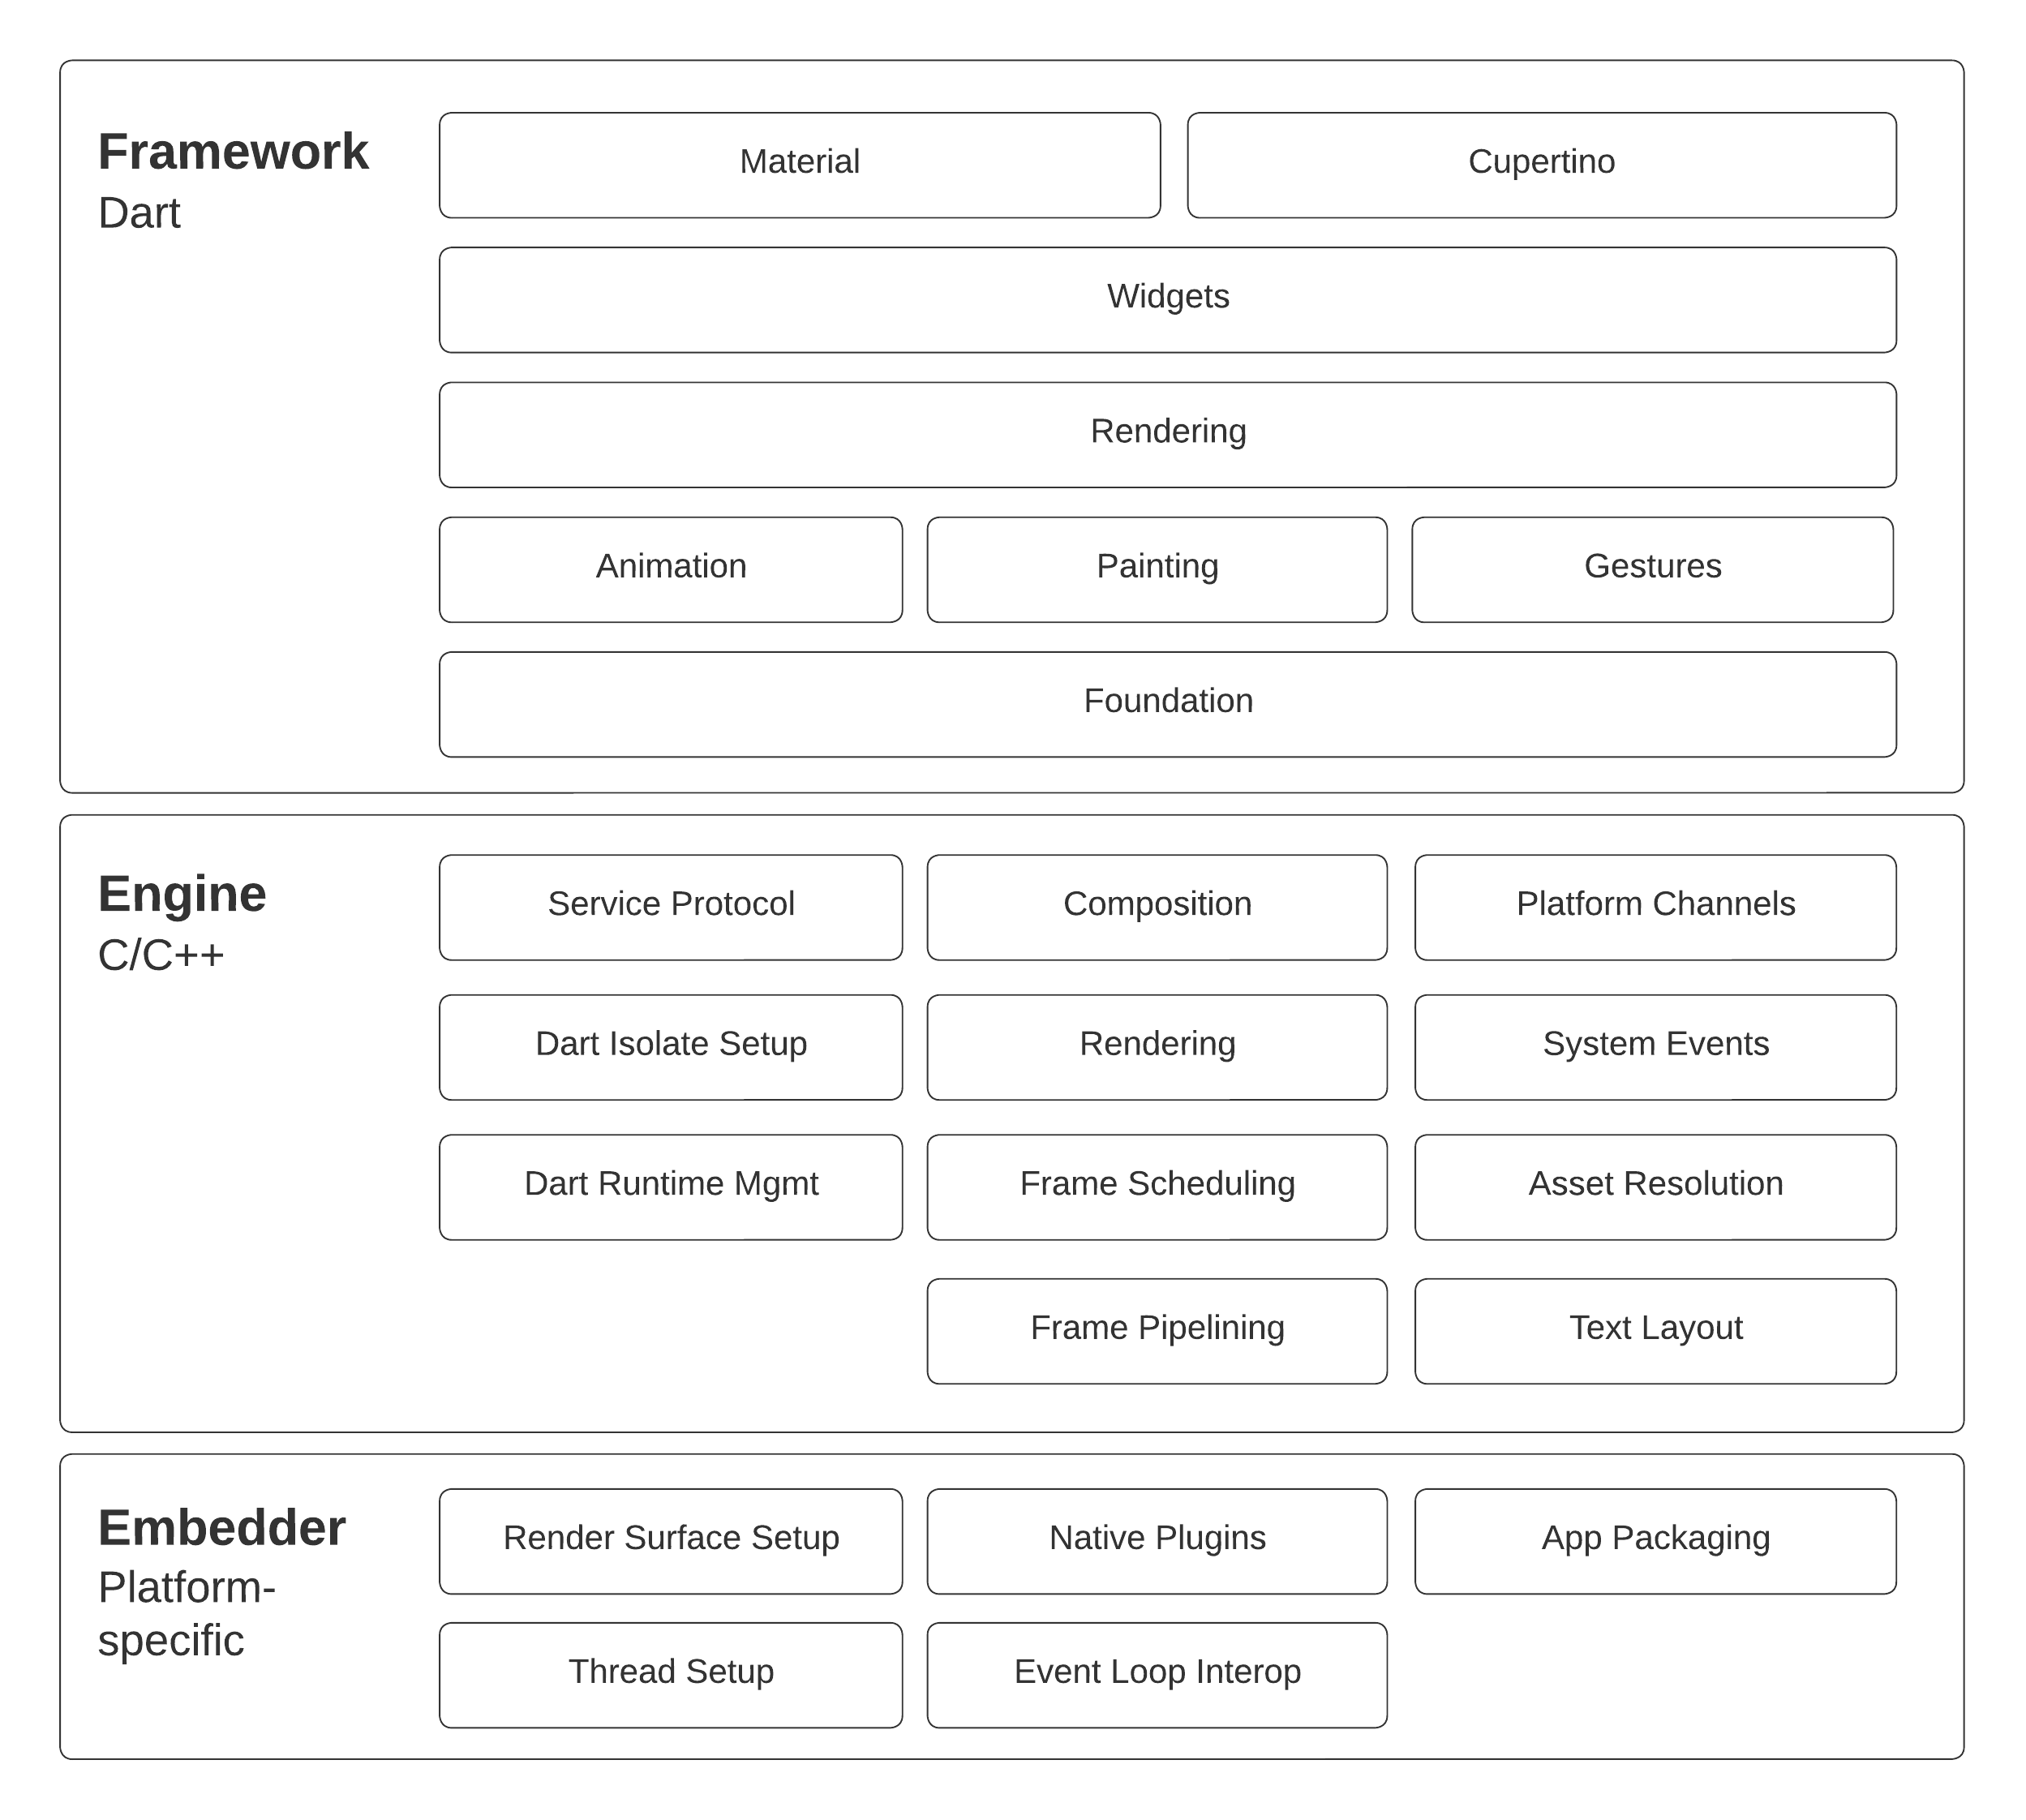
\includegraphics[width = 0.8\textwidth]{images/archdiagram}
	\caption{Straturile arhitecturale ale limbajului Dart}
\end{figure}
\vspace{15pt}
Principala unitate pe care se bazează Flutter este reprezentată de Widget-uri. Acestea sunt colecții de elemente grafice predefinite de către dezvoltatorii Framework-ului. Sunt incluse toate elemente grafice majore, astfel că programatorii care vor să realizeze aplicații utilizând Flutter au la dispoziție toate uneltele necesare. Aceste widget-uri au un grad foarte mare de personalizare. Utilizatorii pot să își creeze propriile widget-uri, pe care ulterior le pot reutiliza. Acestea seamănă într-un fel cu funcțiile din programarea clasică, fiind definite odată, astfel putând fii reapelate ori de câte ori este necesar. Widget-urile funcționează pe un sistem ierarhic. Aproape fiecare widget există în interiorul altui widget printr-un sistem de tip copil - părinte. Toate fac parte dintr-o structură, iar la baza aceste structuri există widget-ul \emph{MaterialApp}. 

Widget-urile sunt de două tipuri: \emph{stateful} și \emph{stateless}. Widget-urile stateless sunt widget-uri care nu își modifică atributele pe parcursul rulării aplicației. Un exemplu bun sunt butoanele de pe bara de navigare sau anumite texte. Widget-urile de tip stateful sunt widget-uri care își modifică forma în funcție de interacțiunea pe care o are utilizatorul. Ca exemplu putem să dăm un formular care afișează diferite valori în funcție de opțiune selectată. În momentul în care o valoare se modifică într-un widget, acesta trebuie să fie reconstruit și reîncărcat, însă acest lucru nu trebuie să fie observat de utilizator. Pentru realizarea acestei operații se apelează semnalul \emph{setState()}, ceea ce indică framework-ului că s-a realizat o modificare și trebuie să reîncarce doar acel widget în particular, fără să reîncarce întreaga fereastră. \cite{flutter:2023}
\newpage
\section{Node.js}
Pentru realizarea părții de Backend a fost utilizat Node.js. Acesta este un mediu de rulare al JavaScript-ului și este utilizat pentru a rula cod de JavaScript în exteriorul unui browser. A fost creat de către Ryan Dahl în anul 2009. Principalele caracteristici ale Node.js-ului sunt faptul că este asincron, are o arhitectură bazată pe un singur fir de execuție, este scalabil, este compatibil cu o multitudine de platforme, și folosește intensiv JavaScript, ceea ce înseamnă că este ușor de învățat. 

Arhitectura limbajului este bazată pe un singur fir de execuție. Acest lucru permite rularea unui număr mare de evenimente simultane. În figura 2.2 se poate vedea o reprezentare grafică a arhitecturii Node.js-ului. \cite{nodejs:2023}
\begin{figure}[H]
    	\centering
    	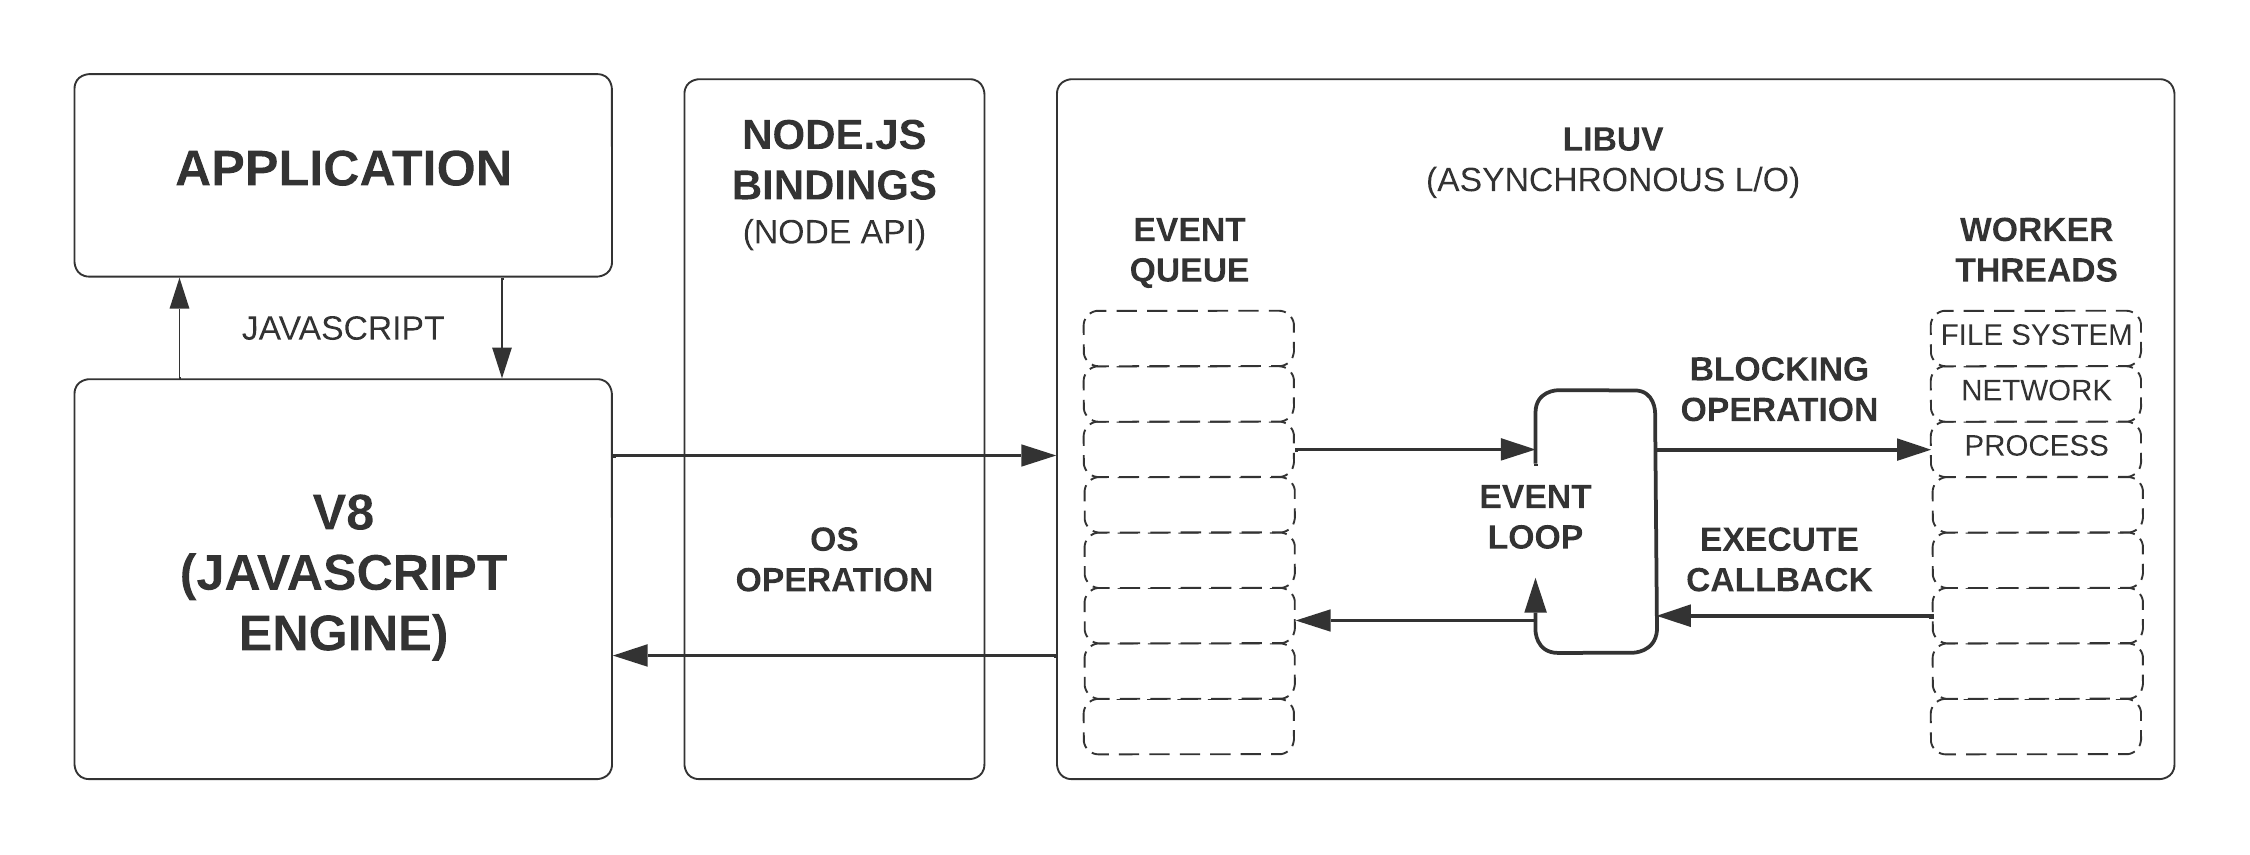
\includegraphics[width = 0.8\textwidth]{images/nodejs}
	\caption{Arhitectura Node.js}
\end{figure}
\section{REST API}
RESTful API se referă la un stil arhitectural specific pentru realizarea unor interfețe de programare (API). Acesta se folosește de protocolul HTTP (Hypertext Transfer Protocol) pentru a accesa informații. Principalele instrucțiuni pe care le folosește sunt GET, PUT, POST și DELETE. Instrucțiunea GET este utilizată pentru a extrage informații, instrucțiunea PUT este utilizată pentru a modifica resursele puse la dispoziție, instrucțiunea POST este folosită pentru a crea o resursă nouă, iar instrucțiunea DELETE este utilizată pentru a șterge o resursă. 

REST API este preferat de obicei față de alte opțiuni similare. Acest lucru se datorează faptului că este foarte eficient, folosind o lățime de bandă relativ redusă. Majoritatea limbajelor de programare moderne suportă acest standard, fiind o opțiune foarte bună în general. \cite{restapi:2020} 

REST API a fost folosit pentru comunicarea cu Backend-ul. Prin intermediul acestui API aplicația extrage și introduce informații în baza de date. Majoritatea componentelor din Backend sunt în format JSON, ceea ce face foarte facilă comunicarea print intermediul REST API-ului. 
\newpage
\section{MongoDB}
Baza de date folosită în realizarea proiectului este creată prin intermediul MongoDB. MongoDB este un tip de baze de date NoSQL. Acesta își stochează informațiile în niște fișiere asemănătoare cu JSON-urile (BSON). MongoDB a fost dezvoltat în 2007 de către compania numită 10gen. În prezent și-au schimbat denumirea în MongoDB Inc. 

În general, MongoDB este utilizat împreună cu JavaScript, dar este folosit și în lucrul cu Node.js, Python sau PHP. Diferența majoră față de SQL este că nu folosește tabele structurale, ceea ce înseamnă că dezvoltatorul poate să stocheze ce vrea în interiorul structurilor de date. MongoDB stochează documentele de tip JSON în colecții, acestea fiind alternativa tabelelor tradiționale din SQL. 

Principalele caracteristici ale acestor baze de date sunt: performanța mare, utilizarea Query API-ului, scalabilitate orizontală și faptul că are un suport dezvoltat pentru diferite soluții de stocare. În figura 2.3 se poate vedea un exemplu al modului în care sunt structurate fișierele JSON în bazele de date de tip MongoDB. \cite{mongodb1:2020} \cite{mongodb2:2020} \cite{mongodb3:2023}
\begin{center}
\begin{figure}[H]
    	\centering
    	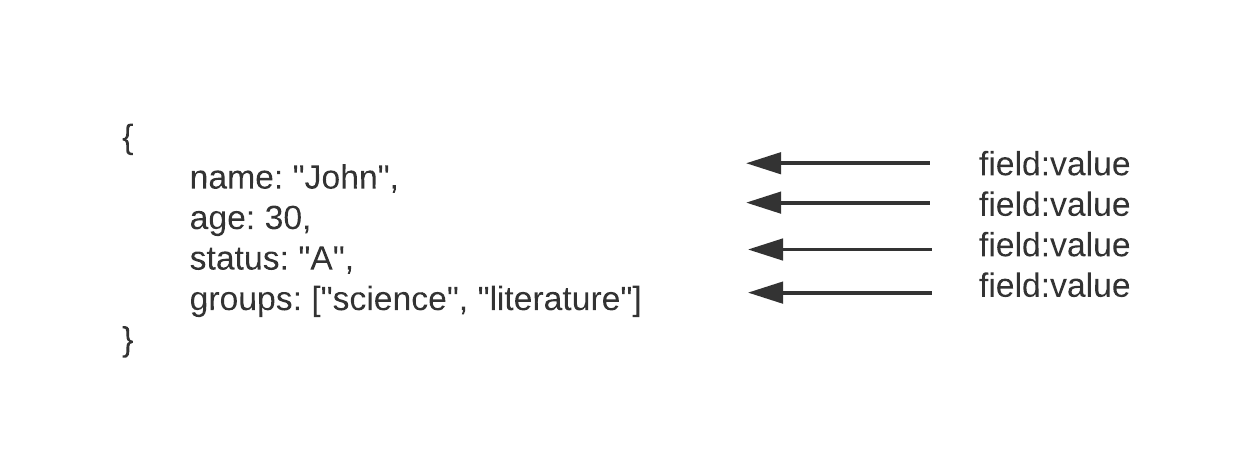
\includegraphics[width = 1\textwidth]{images/mongodb}
	\caption{Exemplu de JSON}
\end{figure}
\end{center}
\chapter{Arhitectura aplicației}
Aplicația este dezvoltată prin intermediul arhitecturii \textbf{Model, View, Controller (MVC)}. Acest tip de arhitectură împarte aplicația în trei componente principale: Model, View și Controller. Fiecare componentă are un scop important, bine definit. Acest tip de arhitectură este foarte des utilizat în dezvoltarea aplicaților mobile sau Web.

În cadrul acestei aplicații, partea de \textbf{Model} se ocupă de stocarea informațiilor legate de conturile de utilizator, respectiv informațiile legate de plângeri. Au fost definite structuri care să poată să țină informațiile extrase din baza de date. Acestea includ toate câmpurile prezente și în baza de date, dar și diferite funcții create pentru manipularea acelor date în cazul în care este necesar. Sunt folosite structuri de date similare și în cazul în care trebuie trimise informații de la aplicație către baza de date.

Partea de \textbf{View} se ocupă de toate componentele vizuale cu care interacționează utilizatorul. Acest lucru include toate ecranele vizibile, incluzând toate butoanele, iconițele și câmpurile pe care le folosește utilizatorul să interacționeze cu aplicația. Acesta are disponibil două ecrane destinate autentificării în contul său de utilizator, sau crearea unui cont în cazul în care nu are, un ecran principal, care conține toate plângerile pe care le-a creat, ecrane informative care conțin diferite date menite să îl ajute în procesul de compunere a unei plângeri, precum și diferite formulare utilizate în crearea unei plângeri sau editarea informațiilor introduse.

Partea de \textbf{Controller} se ocupă de funcționalitatea propriu-zisă a informațiilor introduse prin intermediul componentei \textbf{View}. Această funcționalitate este prezentă în mare parte în componenta de Backend a aplicației. Prin aceste funcționalități, este posibilă autentificarea, crearea de conturi, crearea de plângeri, editarea acestor plângeri, modificarea statusului acestor plângeri în cadrul conturilor de avocați și generarea de plângeri în formatul PDF.

\begin{figure}[H]
    	\centering
    	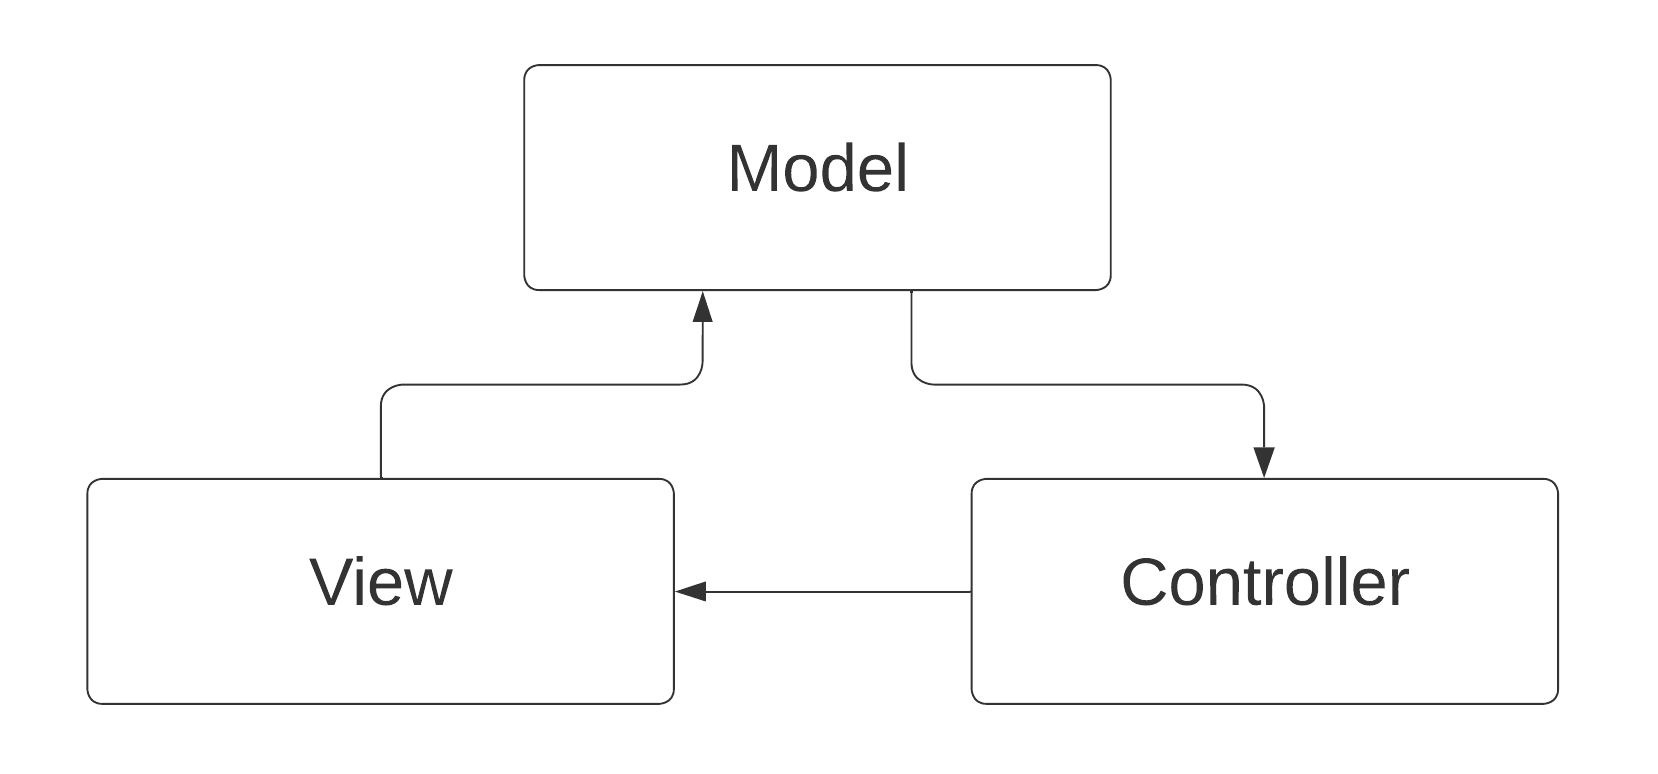
\includegraphics[width = 0.55\textwidth]{images/MVC}
	\caption{Arhitectura MVC}
\end{figure}
\newpage
\section{Baza de date}
\vspace{20pt}
Baza de date care facilitează funcționarea aplicației este realizată prin intermediul platformei MongoDB. Bazele de date sunt de tip NoSQL, ceea ce înseamnă că nu sunt stocate într-un format tabelar, ci în niște fișiere foarte asemănătoare cu formatul JSON.

Principalele fișiere utilizate în cadrul aplicației sunt: \textbf{users}, \textbf{policedepartments} și \textbf{complaints}. Fișierele \textbf{complaints} și \textbf{users} sunt legate între ele prin userID, deoarece fiecare plângere introdusă în baza de date are atribuită un user, acela fiind autorul care a creat acea plângere.

Fișierul \textbf{users} este fișierul în care sunt stocate informațiile legate de conturile de utilizator. Câmpurile prezente în acest fișier sunt: \emph{\_id} (generat în mod automat în momentul creării contului), \emph{Name}, \emph{Surname}, \emph{Password} și \emph{Role}. Conținutul câmpului Password nu este vizibil de către nimeni deoarece conținutul este criptat, pentru a adăuga un grad de securitate.

Fișierul \textbf{policedeparments} conține informații despre un număr mare de secții de poliție din România. Acesta este folosit în cadrul formularului în care sunt introduse datele despre amenda primită de către utilizator. Câmpurile din acest fișier sunt: \emph{County}, \emph{City}, \emph{Name}, \emph{Adress}, \emph{Phone}.

Ultimul fișier este \textbf{complaints}. În acest fișier sunt stocate toate plângerile pe care le au utilizatorii. Acesta poate să fie accesat doar prin intermediul id-ului pe care îl are utilizatorul care a creat plângerea. Acest fișier are cele mai multe câmpuri deoarece trebuie să stocheze o cantitate mare de date pentru fiecare plângere. Câmpurile prezente în acest fișier sunt: \emph{\_id}, \emph{Name}, \emph{Surname}, \emph{Phone}, \emph{Email}, \emph{CIseries}, \emph{CInr}, \emph{CNP}, \emph{City}, \emph{County}, \emph{Street}, \emph{Bl}, \emph{Sc}, \emph{Ap}, \emph{PoliceName}, \emph{PoliceSurname}, \emph{PoliceInstitution}, \emph{PoliceAdr}, \emph{EventPlace}, \emph{VerbalProcess}, \emph{SeriesVerbalProcess}, \emph{NumberVerbalProcess}, \emph{DateVerbalProcess}, \emph{HandingOutVerbalProcess}, \emph{DateOfHandingOutVerbalProcess}, \emph{DateOfEvent}, \emph{PayTheFine}, \emph{Options}, \emph{DescriptionOfTheEventInVerbalProcess}, \emph{DescriptionOfTheEventInPersonalOpinion}, \emph{LawNumberEvent}, \emph{LawParagraphEvent}, \emph{LawRuleEvent}, \emph{LawNumberPay}, \emph{LawParagraphPay}, \emph{LawRulePay}, \emph{Witnesses}, \emph{WitnessesData}, \emph{Judge}, \emph{Lawyer}, \emph{Accept}, \emph{Pay}, \emph{UserID}, \emph{Title}, \emph{Observations}, \emph{Status}

Toate elementele din fișiere sunt de tip String. În cazul în care este necesar un alt tip de date, se face conversia în codul din partea de Frontend.

Pentru modificarea datelor din bazele de date au fost folosite instrucțiuni disponibile în cadrul REST API. Acestea au fost legate de niște endpoint-uri definite în componenta de Backend. Pentru introducerea datelor au fost apelate funcții de \textbf{post}. Acestea au primit niște structuri de date în format JSON definite pentru fiecare componentă din baza de date. Pentru modificarea datelor, au fost folosite funcții de \textbf{put} sau de \textbf{patch}. Acestea operează într-un mod asemănător cu operația de \textbf{post}, folosind o structură de date specifică fiecărui fișier din baza de date. Pentru ștergerea datelor este utilizată funcția de \textbf{delete}, aceasta necesitând doar id-ul obiectului de șters.
\newpage
\section{Diagrama bazei de date}
\vspace{30pt}
\begin{center}
\begin{figure}[H]
    	\centering
    	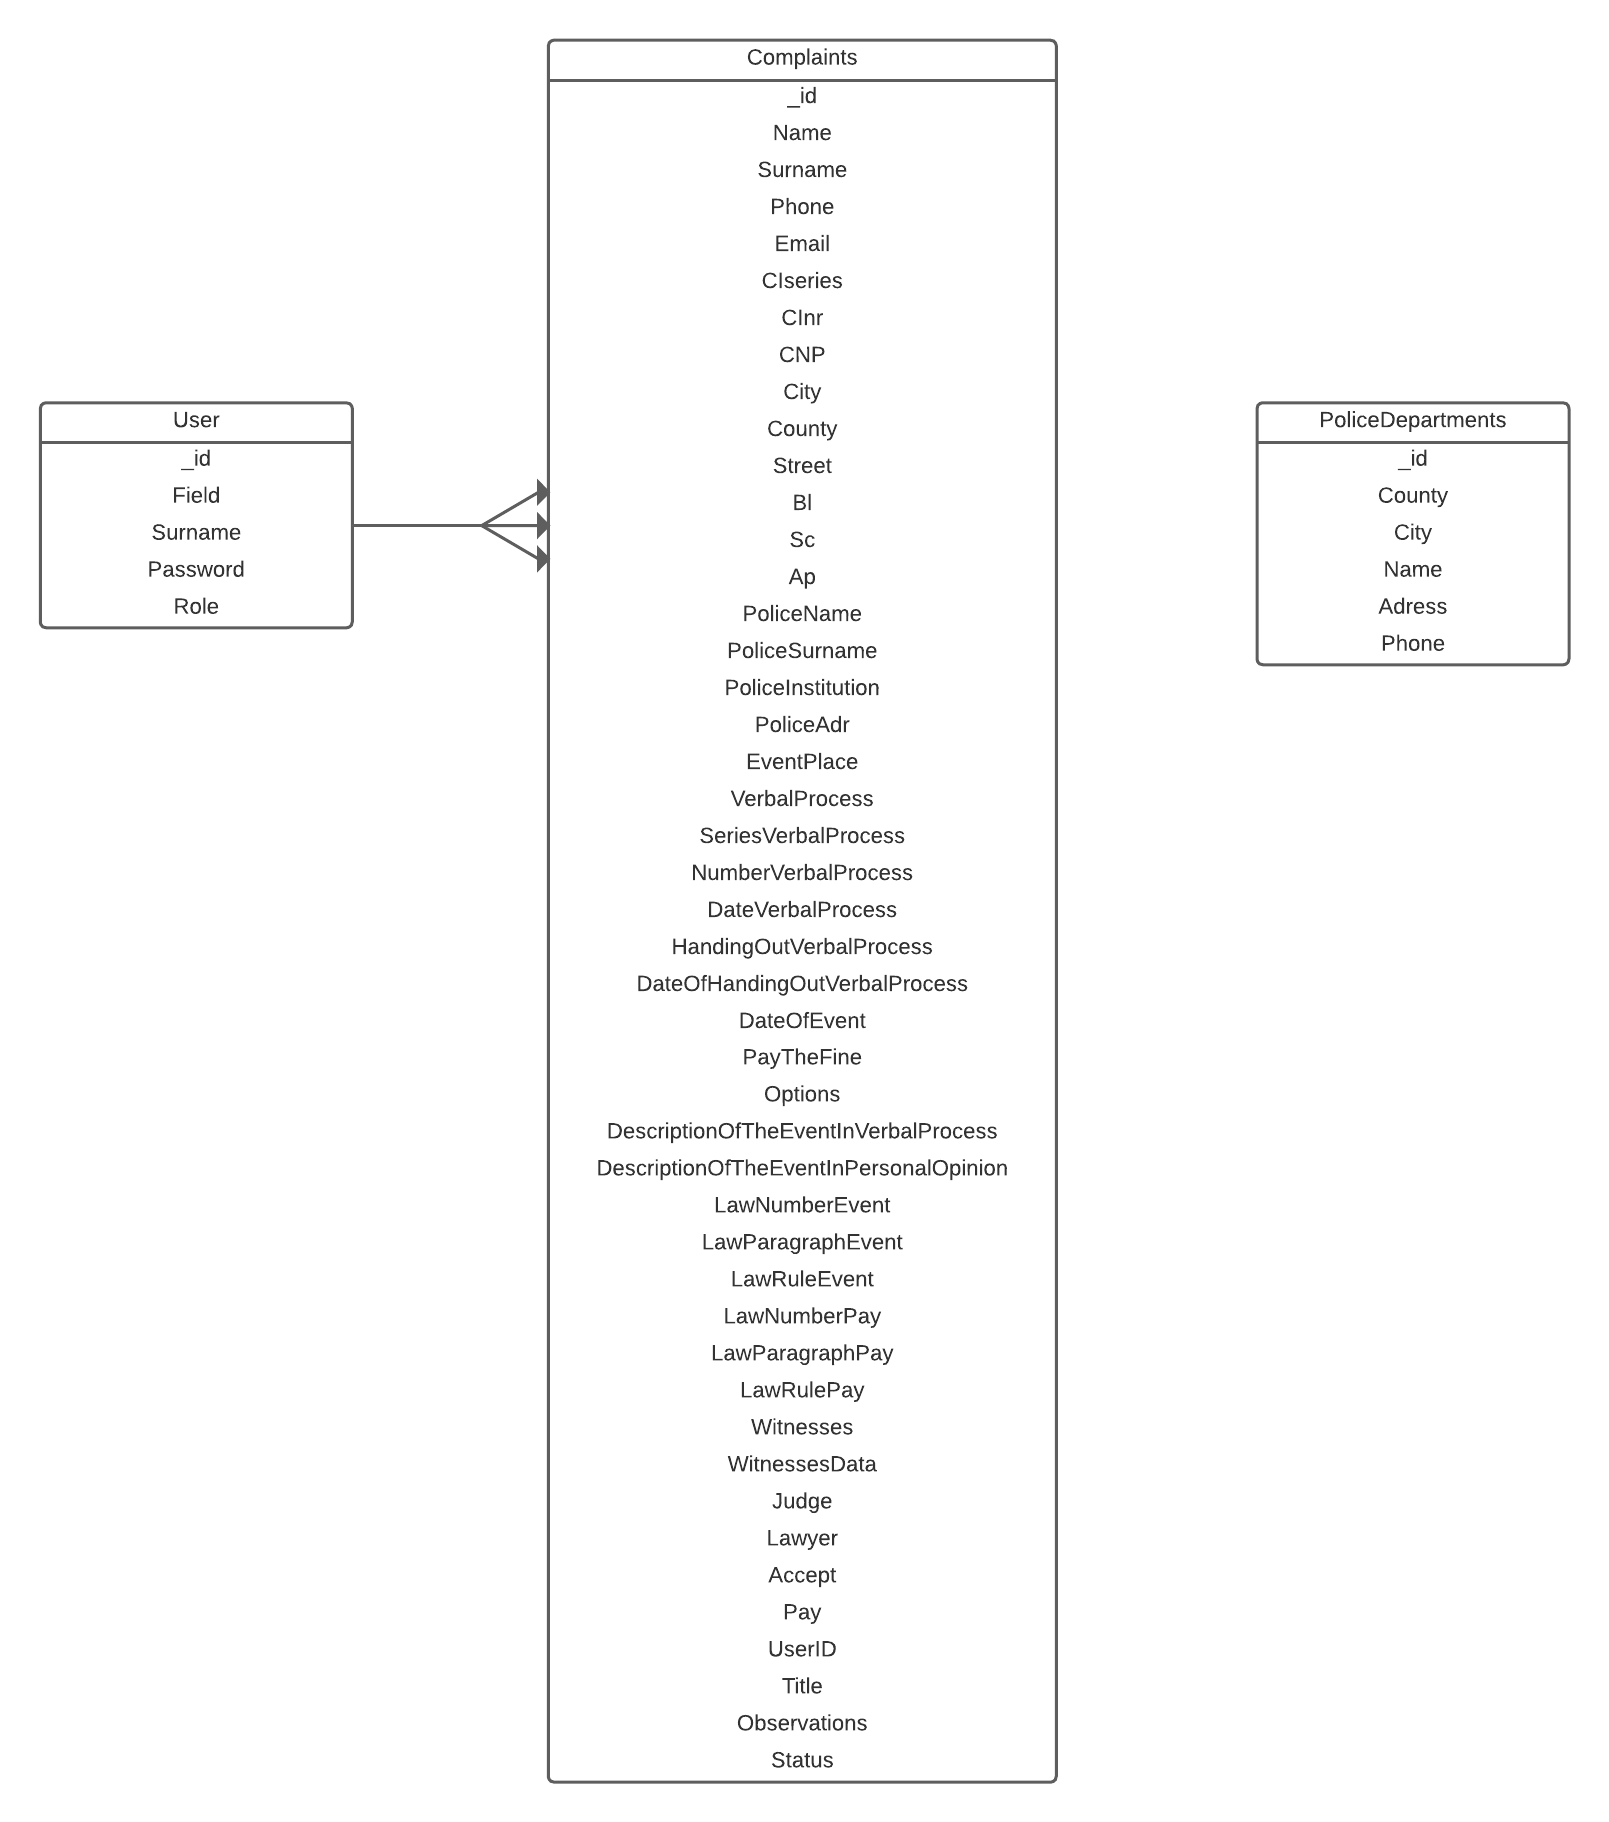
\includegraphics[scale=0.6]{images/erd}
	\caption{Diagrama bazei de date}
\end{figure}
\end{center}
Diagrama de mai sus prezintă principalele elemente prezente în baza de date. Diagrama nu prezintă atâtea detalii deoarece bazele de date de tip NoSQL sunt mult mai relaxate, și nu conțin atâtea restricții și relații precum bazele de date tradiționale. Toate atributele din toate structurile sunt de tip String.
\newpage
\section{Diagrama cazurilor de utilizare}
\vspace{40pt}
\begin{center}
\begin{figure}[H]
    	\centering
    	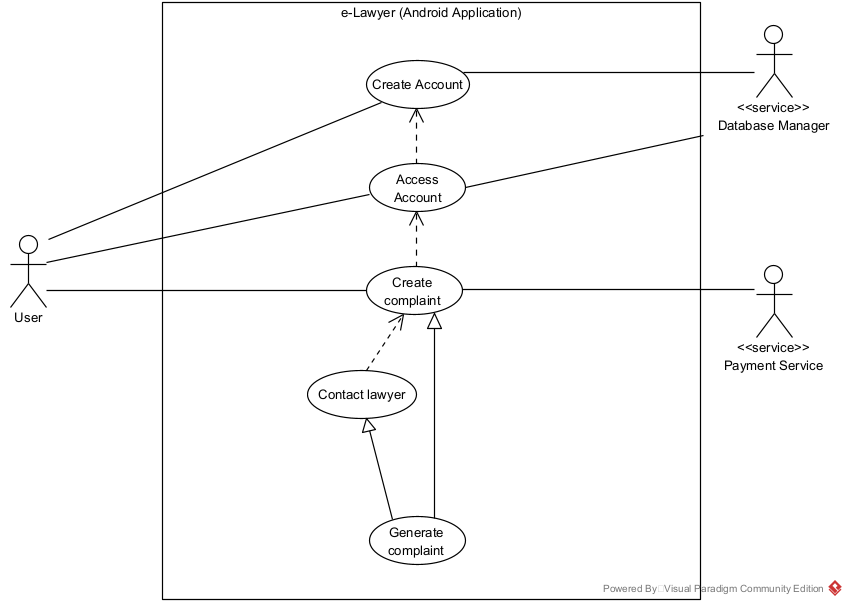
\includegraphics[scale=0.6]{images/e-Lawyer Use Case}
	\caption{Diagrama cazurilor de utilizare}
\end{figure}
\end{center}
\section*{Cazurile de utilizare}
Actorii principali din această structură sunt \textbf{utilizatorul} și \textbf{serviciul de management al bazelor de date}, fiind uneori ajutați de către un serviciu care facilitează sistemul de plăți care este integrat în aplicație.
\begin{itemize}
  \item Utilizatorul inițiază o cerere de creare de cont, această cerere fiind trimisă server-ului în partea de Backend prin intermediul aplicației. Se creează contul și este introdus în baza de date.
  \item Dacă utilizatorul are deja cont, acesta doar își introduce credențialele și așteaptă răspunsul de la baza de date. Aceasta verifică dacă datele sunt corecte, iar în cazul în care utilizatorul este găsit, iar datele sunt introduse corect, utilizatorul primește acces și poate să începe să utilizeze aplicația.
  \item În momentul în care utilizatorul și-a accesat contul, acesta are posibilitatea să creeze contestația legată de amenda primită. Acesta are două opțiuni: să se ocupe de această contestație singur, sau să apeleze la un avocat. În ambele situații trebuie să efectueze o plată (care are tarif diferit în cazul în care utilizatorul lucrează cu un avocat), iar în momentul în care plata este confirmată se pot genera actele necesare după introducerea datelor legate de amendă.

\end{itemize}
\newpage
\section{Diagrama de secvență}
\vspace{30pt}
\begin{center}
\begin{figure}[H]
    	\centering
    	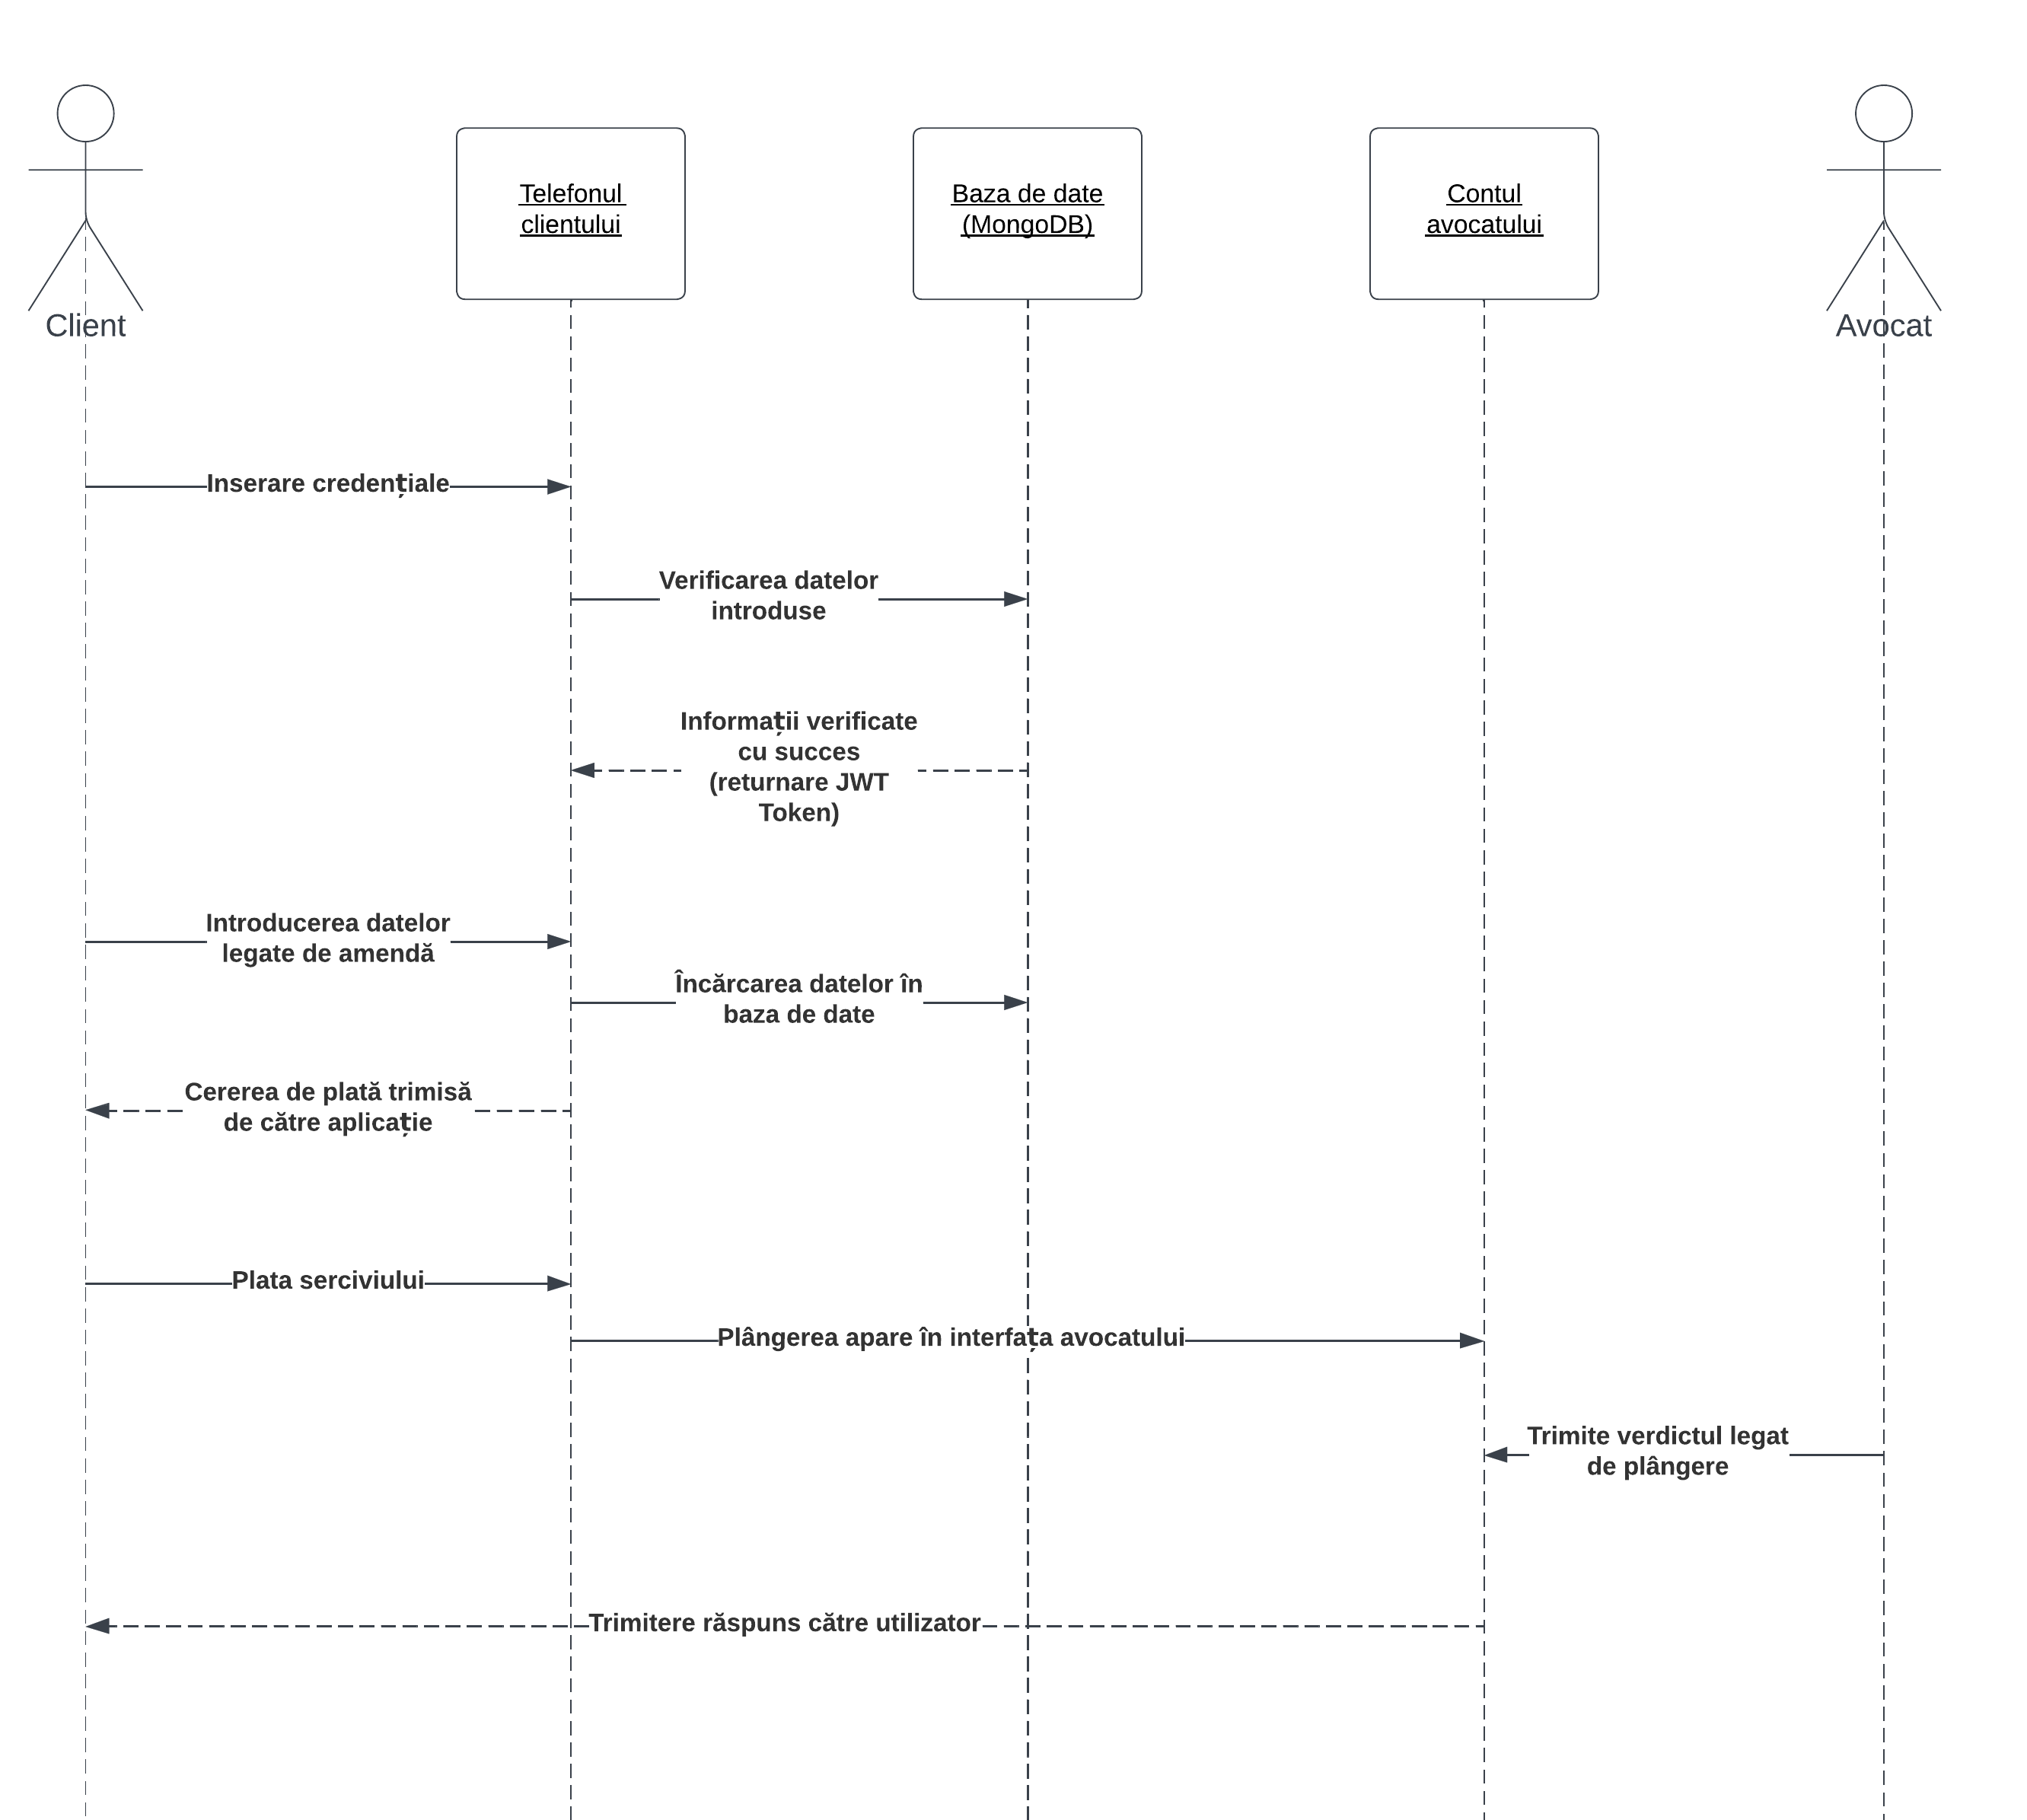
\includegraphics[scale=0.7]{images/seq_diagram.png}
	\caption{Diagrama de secvență}
\end{figure}
\end{center}
Figura de mai sus explică secvența în care se întâmplă acțiunile din aplicație în mod normal. Primul lucru pe care îl face utilizatorul este să se conecteze cu contul de utilizator. Acesta așteaptă un răspuns de la server, acesta fiind reprezentat de un JWT Token care conține datele utilizatorului. În momentul în care utilizatorul a intrat în cont, acesta poate să creeze o plângere. După ce introduce datele necesare, acestea sunt trimise la baza de date pentru a se crea plângerea. Ulterior, clientul este nevoit să plătească serviciul, pentru ca datele să poată să fie trimise către avocat. În momentul în care avocatul a primit datele, poate să dea un răspuns. Acel răspuns este trimis către utilizator, pentru a-l informa în legătură cu ce poate să facă în continuare.
\newpage
\section{Componenta Backend}

Componenta de Backend a aplicației a fost dezvoltată în Node.js. În principal, partea de Backend se ocupă de crearea structurilor în care sunt stocate datele, cât și da manipularea acestora în principal cu ajutorul REST API-ului. În cadrul acestei componente au fost dezvoltate controllere, rute și modele.

Modelele funcționează ca și un schelet pentru datele care urmează să fie manipulate. În cadrul acestor structuri sunt definite caracteristicile pe care le are fiecare obiect definit, tipul de date utilizat, dar și niște restricții în unele cazuri, cum ar fi exact valoarea pe care ar trebui să o ia. Principalele modele definite sunt \emph{Complaint}, \emph{PoliceDepartment} și \emph{User}. 

Rutele (Routes) sunt definite pentru a crea niște endpoint-uri la care se conectează aplicația pentru a extrage sau pentru a modifica diferite informații necesare pentru funcționalitatea completă a acesteia. Pentru fiecare model definit a fost creat un fișier din categoria de rute în care sunt definite endpoint-urile cu ajutorul cărora se fac diferitele operații de tip REST API. Partea de User are definite endpoint-urile \textbf{post/signup} pentru crearea conturilor de utilizator, \textbf{post/login} pentru realizarea autentificării, \textbf{delete}, \textbf{get} și \textbf{patch} pentru realizarea operațiilor de ștergere, extragere a informațiilor și modificarea acestora. PoliceDepartment are definit ca endpoint-uri \textbf{get}, \textbf{post}, \textbf{get/id} și \textbf{patch/id}. Pentru partea de plângeri au fost definite endpoint-uri de \textbf{get} pe baza id-ului plângerii, respectiv pe baza id-ului user-ului care a creat plângerea,  \textbf{post} pentru încărcarea plângerilor după ce au fost create în aplicație, \textbf{put} pentru editarea datelor și \textbf{delete} pentru ștergerea plângerilor.

Controllerele sunt utilizate pentru a defini comportamentul pe care diferitele componente ale aplicației le vor avea. Precum la modele sau la rute, a fost definit câte un fișier de tip controller pentru fiecare componentă prezentată anterior. În controllere sunt definite toate acțiunile care ar trebui făcute în momentul în care endpoint-urile din rute sunt accesate. Modul în care operează aceste acțiuni este de a trimite o cerere către baza de date prin intermediul operațiilor oferite de către REST API, apoi așteaptă un răspuns pe care îl trimite mai deparete.

În controllerul user-ului sunt definite operațiile de \emph{getAllUsers}, \emph{updateUsers}, \emph{getUserById}, \emph{getUserByNameAndSurname}, \emph{createNewUser}, \emph{deleteUser} și \emph{loginUser}. Majoritatea acestor funcții doar apelează operațiile respective căreia i-au fost atribute și trimite înapoi un răspuns care fie este informația căutată, fie un cod de eroare. Funcția de \emph{loginUser} compară adresa de mail și parola care au fost extrase din Frontend și le compară cu informațiile din baza de date. În cazul în care aceste informații coincid, funcția returnează un JWT Token cu informațiile user-ului căutat, printr-o serie de caractere criptate. În cazul în care nu este găsit utilizatorul căutat este returnat un cod de eroare.

Controllerul care se ocupă de partea de plângeri are funcțiile \emph{getComplaintByUserId}, \emph{getComplaintByUserEmail}, \emph{getComplaintById}, \emph{createComplaint}, \emph{updateComplaint}, \emph{updateComplaintByUserId}, \emph{deleteComplaint} și \emph{getComplaint}. Aceste funcții se ocupă în principal de crearea plângerilor, extragerea informațiilor, modificare și ștergerea acestora.

Controllerul intitulat PoliceDepartment se ocupă de informațiile legate de secțiile de poliție. Funcțiile prezente în cadrul acestui controller sunt \emph{getAllPoliceDepartments}, \emph{createNewPoliceDepartment}, \emph{findPoliceDepartmentById}, \emph{updatePoliceDepartment} și \emph{deletePoliceDepartment}.
\newpage
\chapter{Prezentarea aplicației}
\section{Conturile de utilizator}
O parte foarte importantă a aplicației este reprezentată de conturile de utilizator. Acestea sunt de două tipuri, fiecare având un nivel diferit de permisiuni și atribuții:
\begin{itemize}
  \item  Primul tip este contul normal, folosit de majoritatea utilizatorilor. Aceștia au opțiunea să folosească toate facilitățile de bază oferite de către aplicație. Acestea includ crearea de contestații, modificarea detaliilor legate de propriul profil, accesarea vechilor contestații și accesarea informațiilor utile oferite de către aplicație.
  \item  Al doilea tip de cont este cel de avocat. Utilizatorii de tip avocat sunt obligați să ofere un act doveditor care atestă faptul că sunt avocați aprobați de către Barou. Aceștia au acces la mai puține funcții, deoarece atribuția lor este să ajute utilizatorii normali în prezentarea contestației spre judecătorie.
 
\end{itemize}

În momentul în care utilizatorul deschide aplicația are două opțiuni: să se autentifice în contul de utilizator, sau în cazul în care acesta nu are un cont, poate să își creeze unul. Acesta dispune de o interfață intuitivă și ușor de utilizat. Pentru accesarea contului de utilizator sunt cerute doar adresa de mail și parola. Parolele sunt ascunse printr-un algoritm de hashing în Backend pentru un nivel mai ridicat de securitate, astfel că nici măcar administratorul bazelor de date nu poate să vadă date sensibile.

În interiorul aplicației au fost introduse mecanisme de verificare a datelor introduse în momentul creării contului de utilizator. Astfel, un utilizator nu poate introduce o adresă de mail în format eronat,  sau să lase câmpuri necompletate. Aceste verificări au fost introduse pentru a asigura că toate conturile create sunt realizate cu informații corespunzătoare care nu pot să compromită datele utilizatorilor sau funcționarea corectă a aplicației. În figura 4.1 se pot observa câteva exemple ale interfeței grafice care facilitează utilizarea conturilor.
\begin{figure}[H]
  \centering
  \subfloat[Ecranul de Sign In]{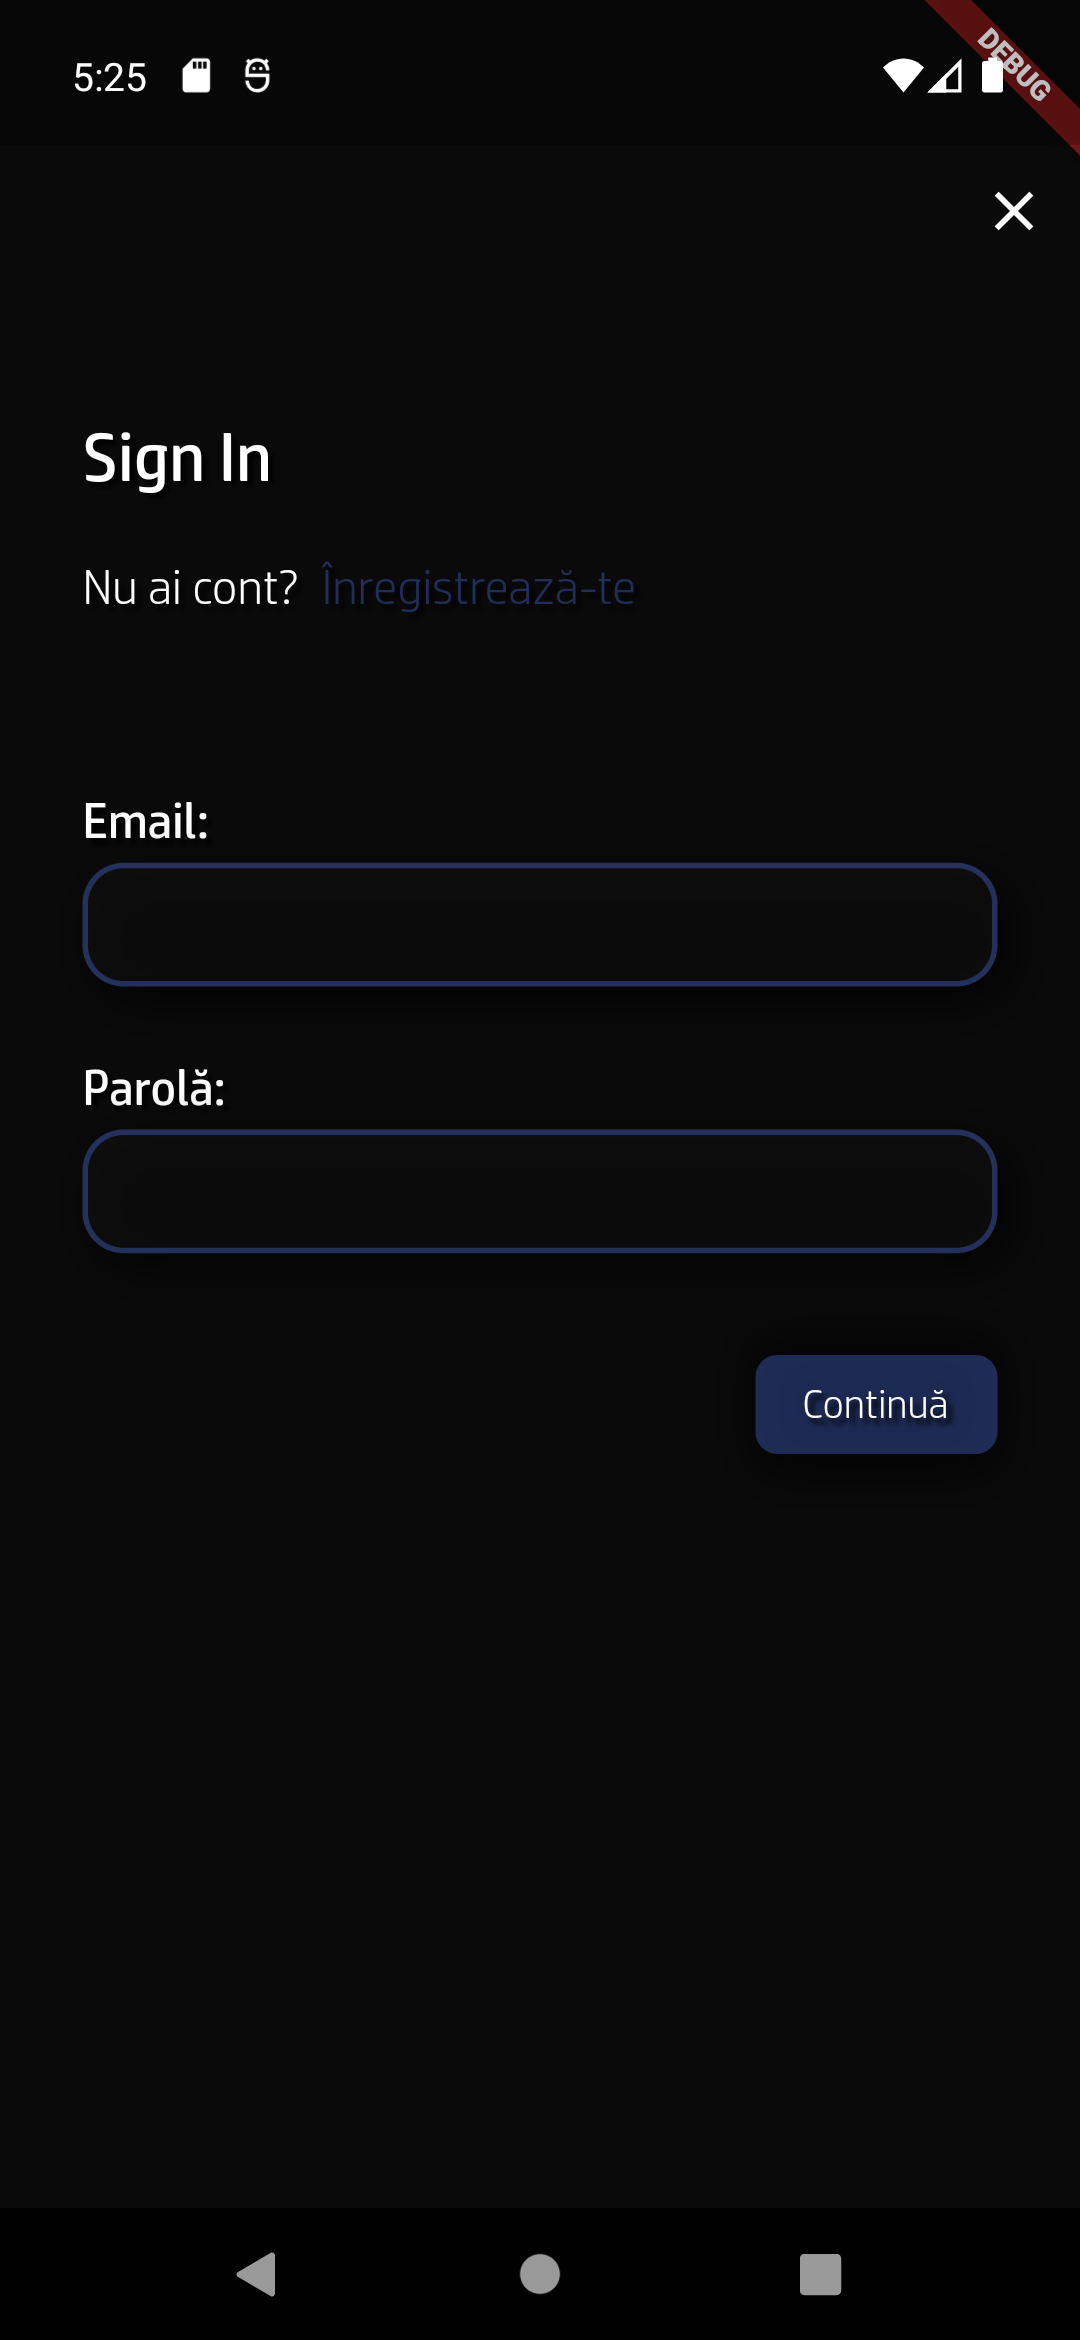
\includegraphics[width=0.3\textwidth]{images/ecran1}}
  \hspace{0.3cm}
  \subfloat[Ecranul de Sign Up]{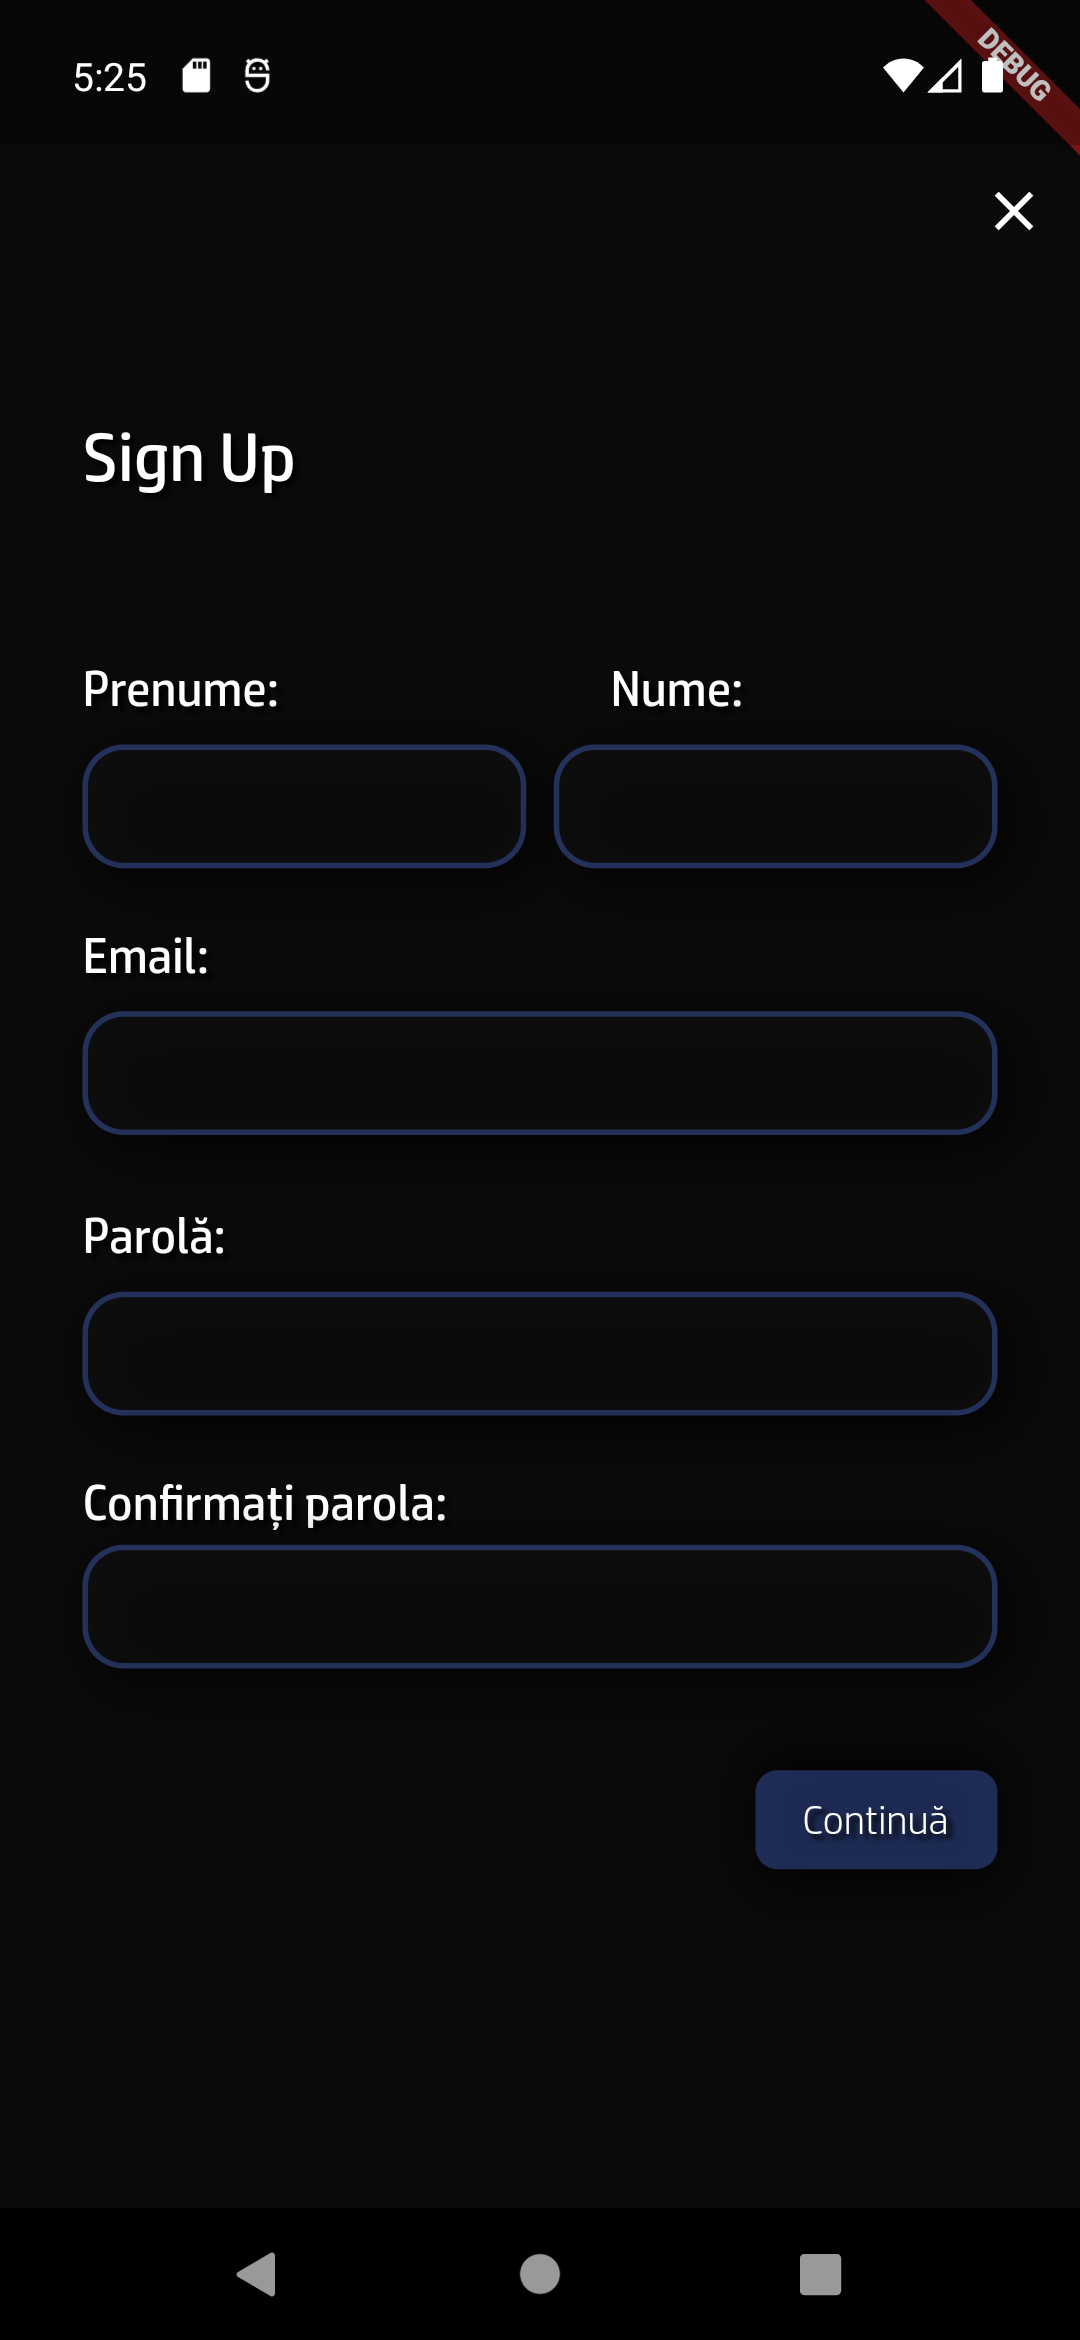
\includegraphics[width=0.3\textwidth]{images/ecran2}\label{fig:f2}}
  \hspace{0.3cm}
  \subfloat[Ecranul de Sign Up cu informații incorecte]{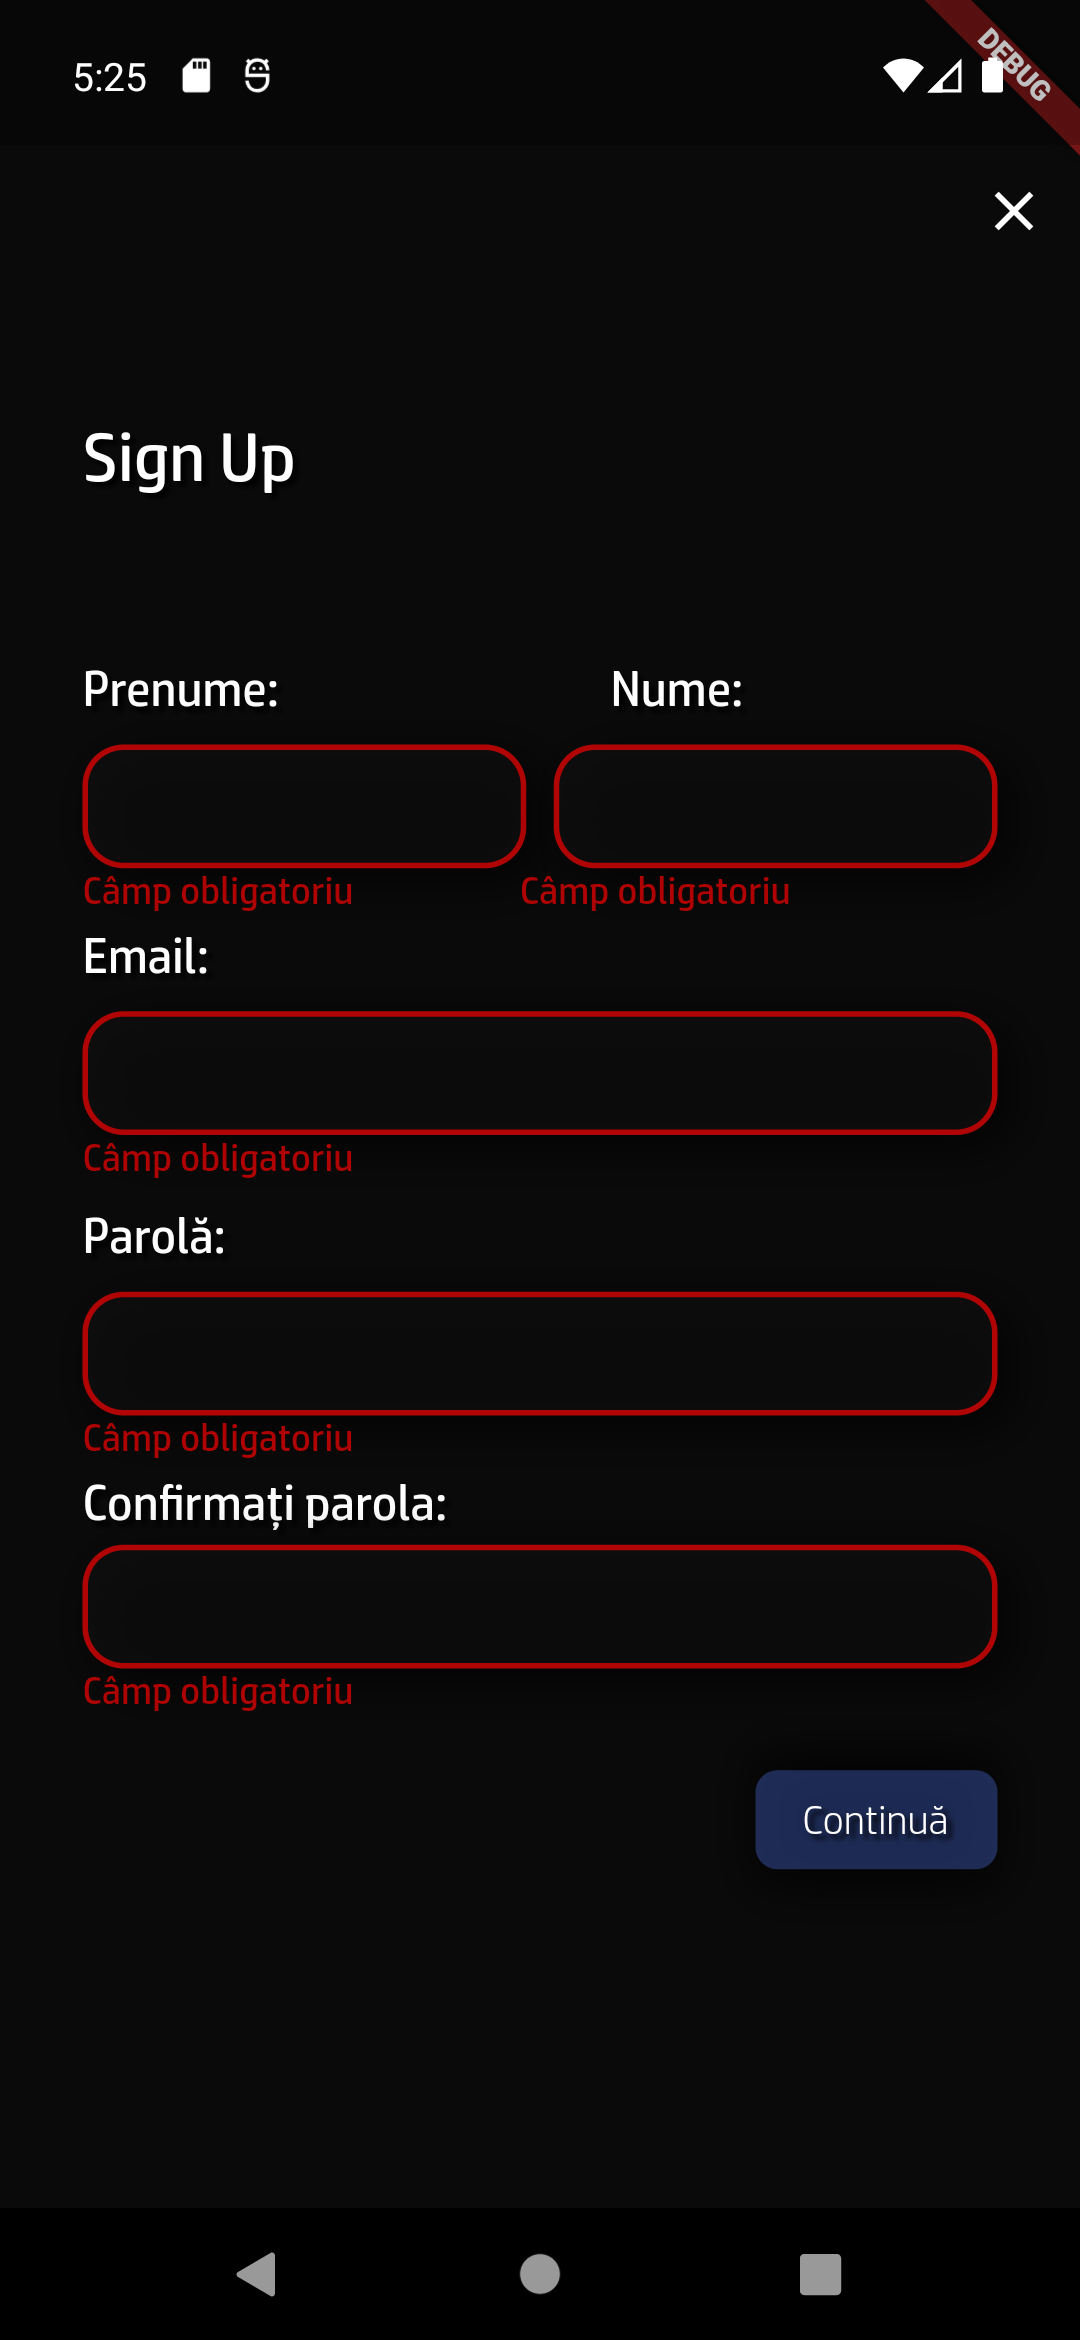
\includegraphics[width=0.3\textwidth]{images/ecran3}\label{fig:f3}}
  \caption{Interfața grafică pentru administrarea conturilor de utilizator}
\end{figure}
Datele stocate în conturile utilizatorilor sunt utilizate pentru identificarea autorilor plângerilor de către avocați. În momentul în care o persoană intră într-un cont de avocat, poate să vadă toate plângerile, la care sunt atribuite atât numele și prenumele, cât și adresa de mail ale utilizatorului care a creat acea plângere. Alte date care sunt salvate în cadrul contului de utilizator sunt plângerile propriu - zise. Acestea sunt în format PDF, iar utilizatorul poate să le descarce ori de câte ori are nevoie. Acesta are și posibilitatea să le editeze, aceste date fiind salvate în cadrul contului său.

Utilizatorul are și posibilitatea să își editeze date din cadrul contului său. În cazul în care acesta a greșit date în momentul creării contului, are mereu posibilitatea să le modifice pentru a se asigura că poate să fie contactat de către avocați. 

Bazele de date în care sunt stocatele datele utilizatorilor sunt încărcate în MongoDB. Comunicarea dintre aplicație și bazele de date este realizată folosind apeluri facilitate de către REST API. Datele sunt preluate de către Frontend prin intermediul unor apeluri de tip get, care se realizează în momentul intrării în contul de utilizator. Acest lucru asigură faptul că tot timpul sunt afișate date actualizate pe ecran. În cazul în care utilizatorul consideră că nu are toate datele actualizate pe ecranul principal al aplicației, are opțiunea să actualizeze datele prin intermediul unui buton de refresh. Datele colectate din baza de date includ nume și prenumele utilizatorului, cât și plângerile pe care le-a creat acesta, ele fiind afișate pe ecranul principal al aplicației. Datele menționate pot să fie actualizate prin intermediul unor funcții de put sau patch, ceea ce conferă un control mai mare al utilizatorilor asupra conturilor lor și a datelor gestionate în cadrul acestor conturi.
\newpage
\section{Meniul principal}
\vspace{20pt}
După ce utilizatorul se autentifică, acesta este redirecționat către meniul principal al aplicației. Acesta este conceput din trei ecrane unite prin intermediul unei bări de navigare poziționată în partea inferioară a ecranului. Principalele elemente ale interfeței sunt:
\begin{itemize}
  \item \textbf{Acasă}: Ecranul principal în care utilizatorul interacționează cu elementele fundamentale ale aplicației. Acesta poate să își vizualizeze plângerile trecute sau să compune o plângere nouă în cadrul acestei ferestre.
  \item \textbf{Profil}: În acest ecran utilizatorul poate să își acceseze datele legate de utilizator. Din acest ecran el poate să se deconecteze din contul său sau să își editeze detaliile legate de contul său. 
  \item \textbf{Meniu}: Meniul acesta este o listă mai detaliată a majorității funcțiilor disponibile în cadrul aplicației. Aici utilizatorul poate să acceseze link-uri cu informații care pot să îl ajute în scrierea contestației, dar și să facă majoritatea lucrurilor de pe celelalte ecrane, rolul acestui meniu fiind să aibă majoritatea informațiilor într-un mod mai concis.
\end{itemize}

\begin{figure}[H]
  \centering
  \subfloat[Ecranul principal]{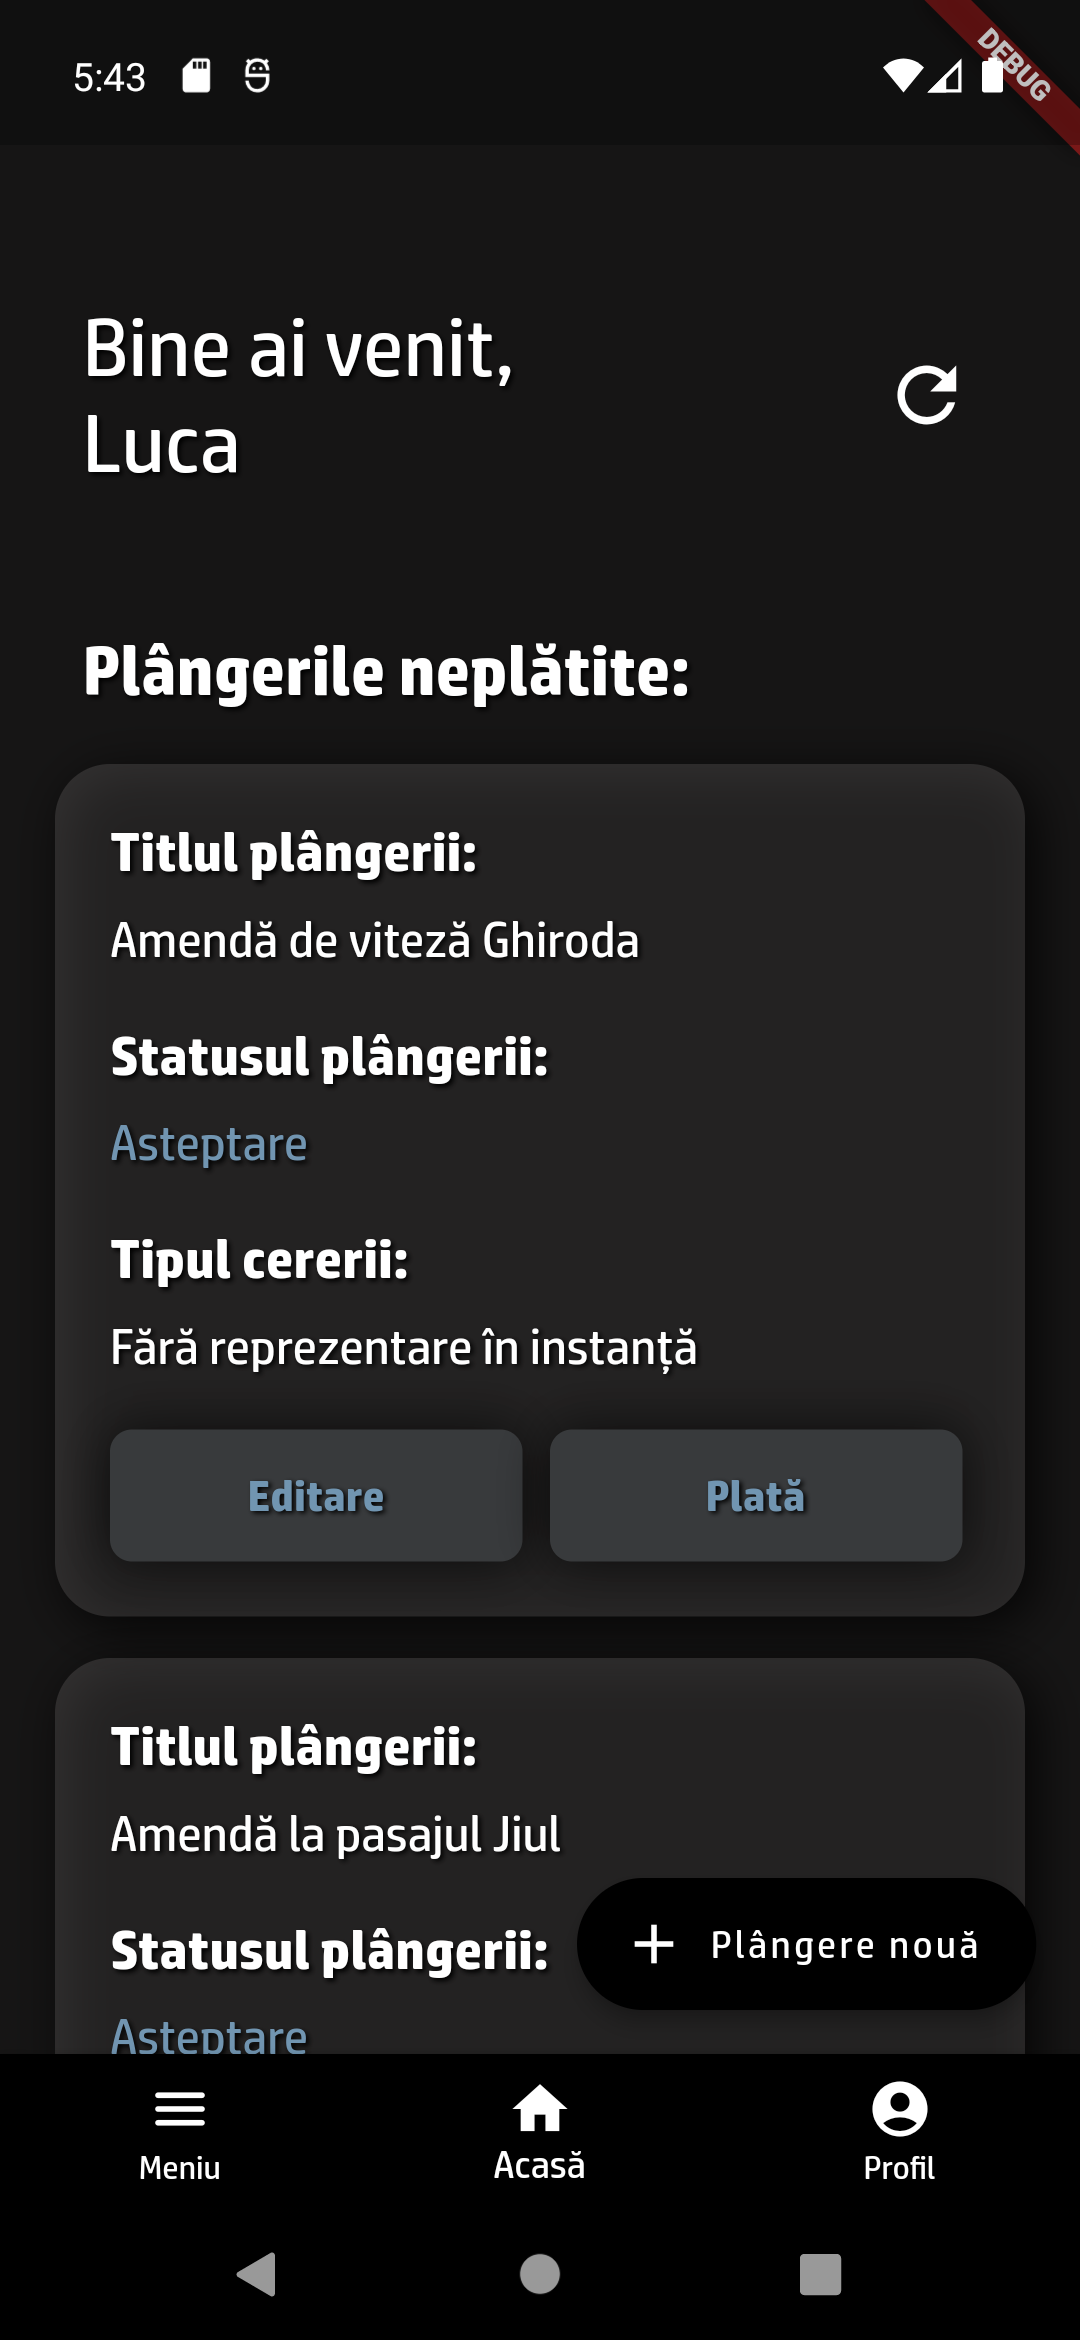
\includegraphics[width=0.3\textwidth]{images/ecran4}}
  \hspace{0.3cm}
  \subfloat[Ecranul Profil]{
\includegraphics[width=0.3\textwidth]{images/ecran5}\label{fig:f2}}
  \hspace{0.3cm}
  \subfloat[Ecranul Meniu]{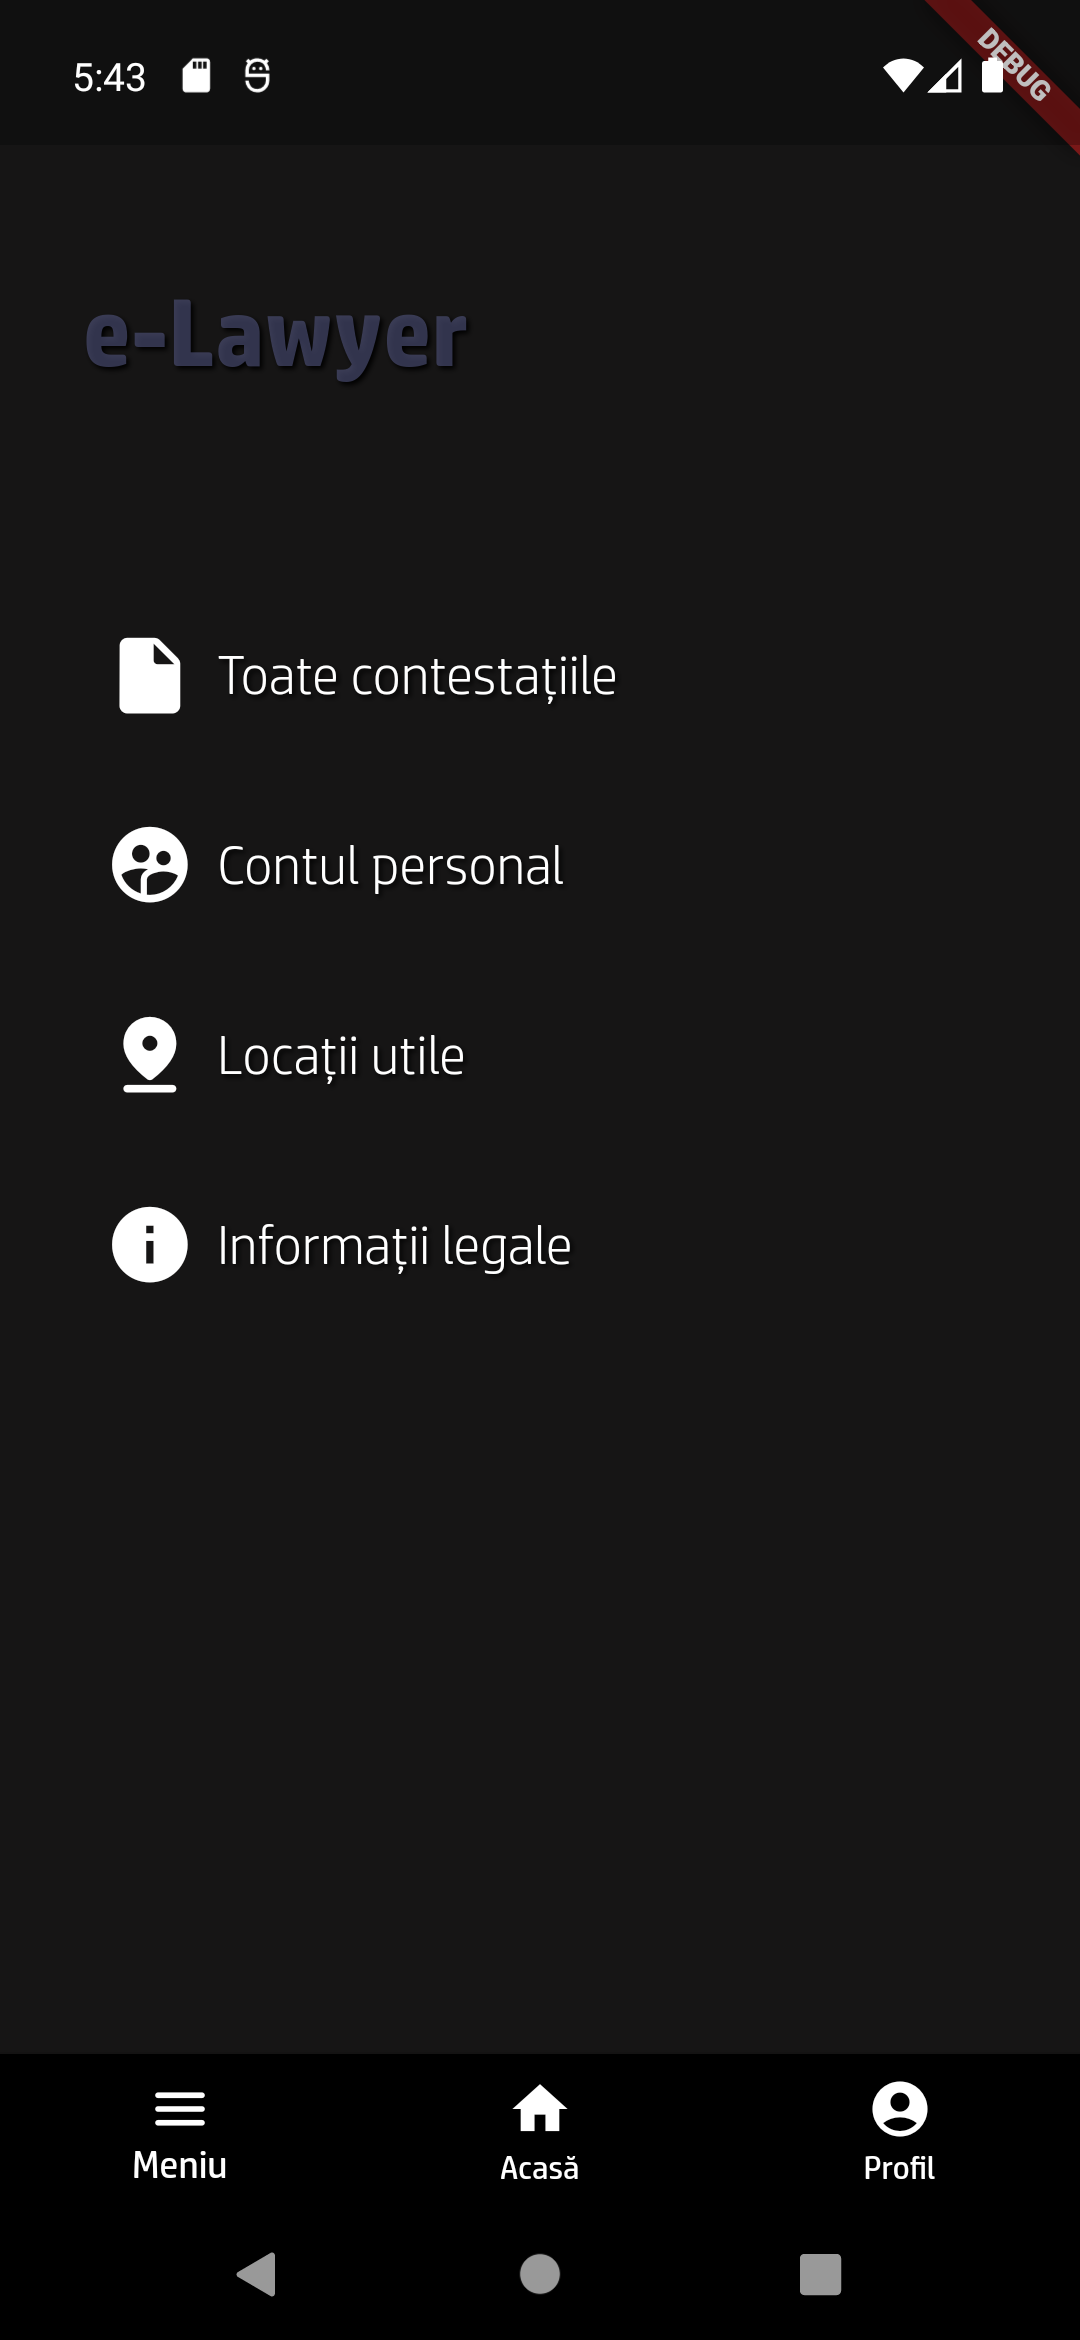
\includegraphics[width=0.3\textwidth]{images/ecran6}\label{fig:f3}}
  \caption{Interfața grafică a meniurilor principale ale aplicației}
\end{figure}
\newpage
\section*{Ecranul principal (Acasă)}
Ecranul principal este elementul central al aplicației cu care se întâlnește utilizatorul prima dată. Menirea lui este de de a avea un comportament asemănător unui panou de control, în care sunt stocate toate plângerile create de către utilizator. Acestea sunt împărțite în două categorii: \textbf{Plângerile neplătite} și \textbf{Plângerile plătite}. Această diferențiere este realizată deoarece doar plângerile plătite sunt cele care ajung să poată să fie vizualizate de către avocați. 

Plângerile sunt afișate pe ecran ca niște cartonașe care include câteva informații utile despre plângerile propriu - zise, precum și câteva butoane care indică acțiunile pe care utilizatorul poate să le facă cu produsul în cauză. Informațiile prezentate includ titlul plângerii, statusul plângerii (care poate să fie Așteptare, Aprobată sau Refuzată) și tipul plângerii. Plângerile pot să fie de două tipuri în funcție de ceea ce dorește utilizatorul: fără reprezentare în instanță de către avocat sau cu reprezentare în instanță de către avocat. Acest lucru este afișat ca una din informațiile principale pe ecran deoarece utilizatorul trebuie să plătească o sumă diferită de bani, în funcție de această alegere. Plângerea în care utilizatorul dorește să fie reprezentat de către un avocat are un preț mai mare decât cea normală, iar acest lucru trebuie să fie prezent în interfața aplicației în mod explicit, pentru ca utilizatorul să se asigure că a ales opțiunile corecte înainte să plătească serviciul prestat. 

Butoanele prin care utilizatorul realizează diferite acțiuni legate de aceste plângeri diferă dacă această plângere a fost plătită sau de statusul în care această plângere este. Inițial, utilizatorul are opțiunea să editeze datele din plângere, dar și să plătească serviciul. În momentul în care utilizatorul apasă butonul de editare este redirecționat către un ecran în care sunt prezentate toate informațiile introduse de către utilizator legate de plângerea selectată.
\begin{figure}[H]
  \centering
  \subfloat[Editarea plângerilor]{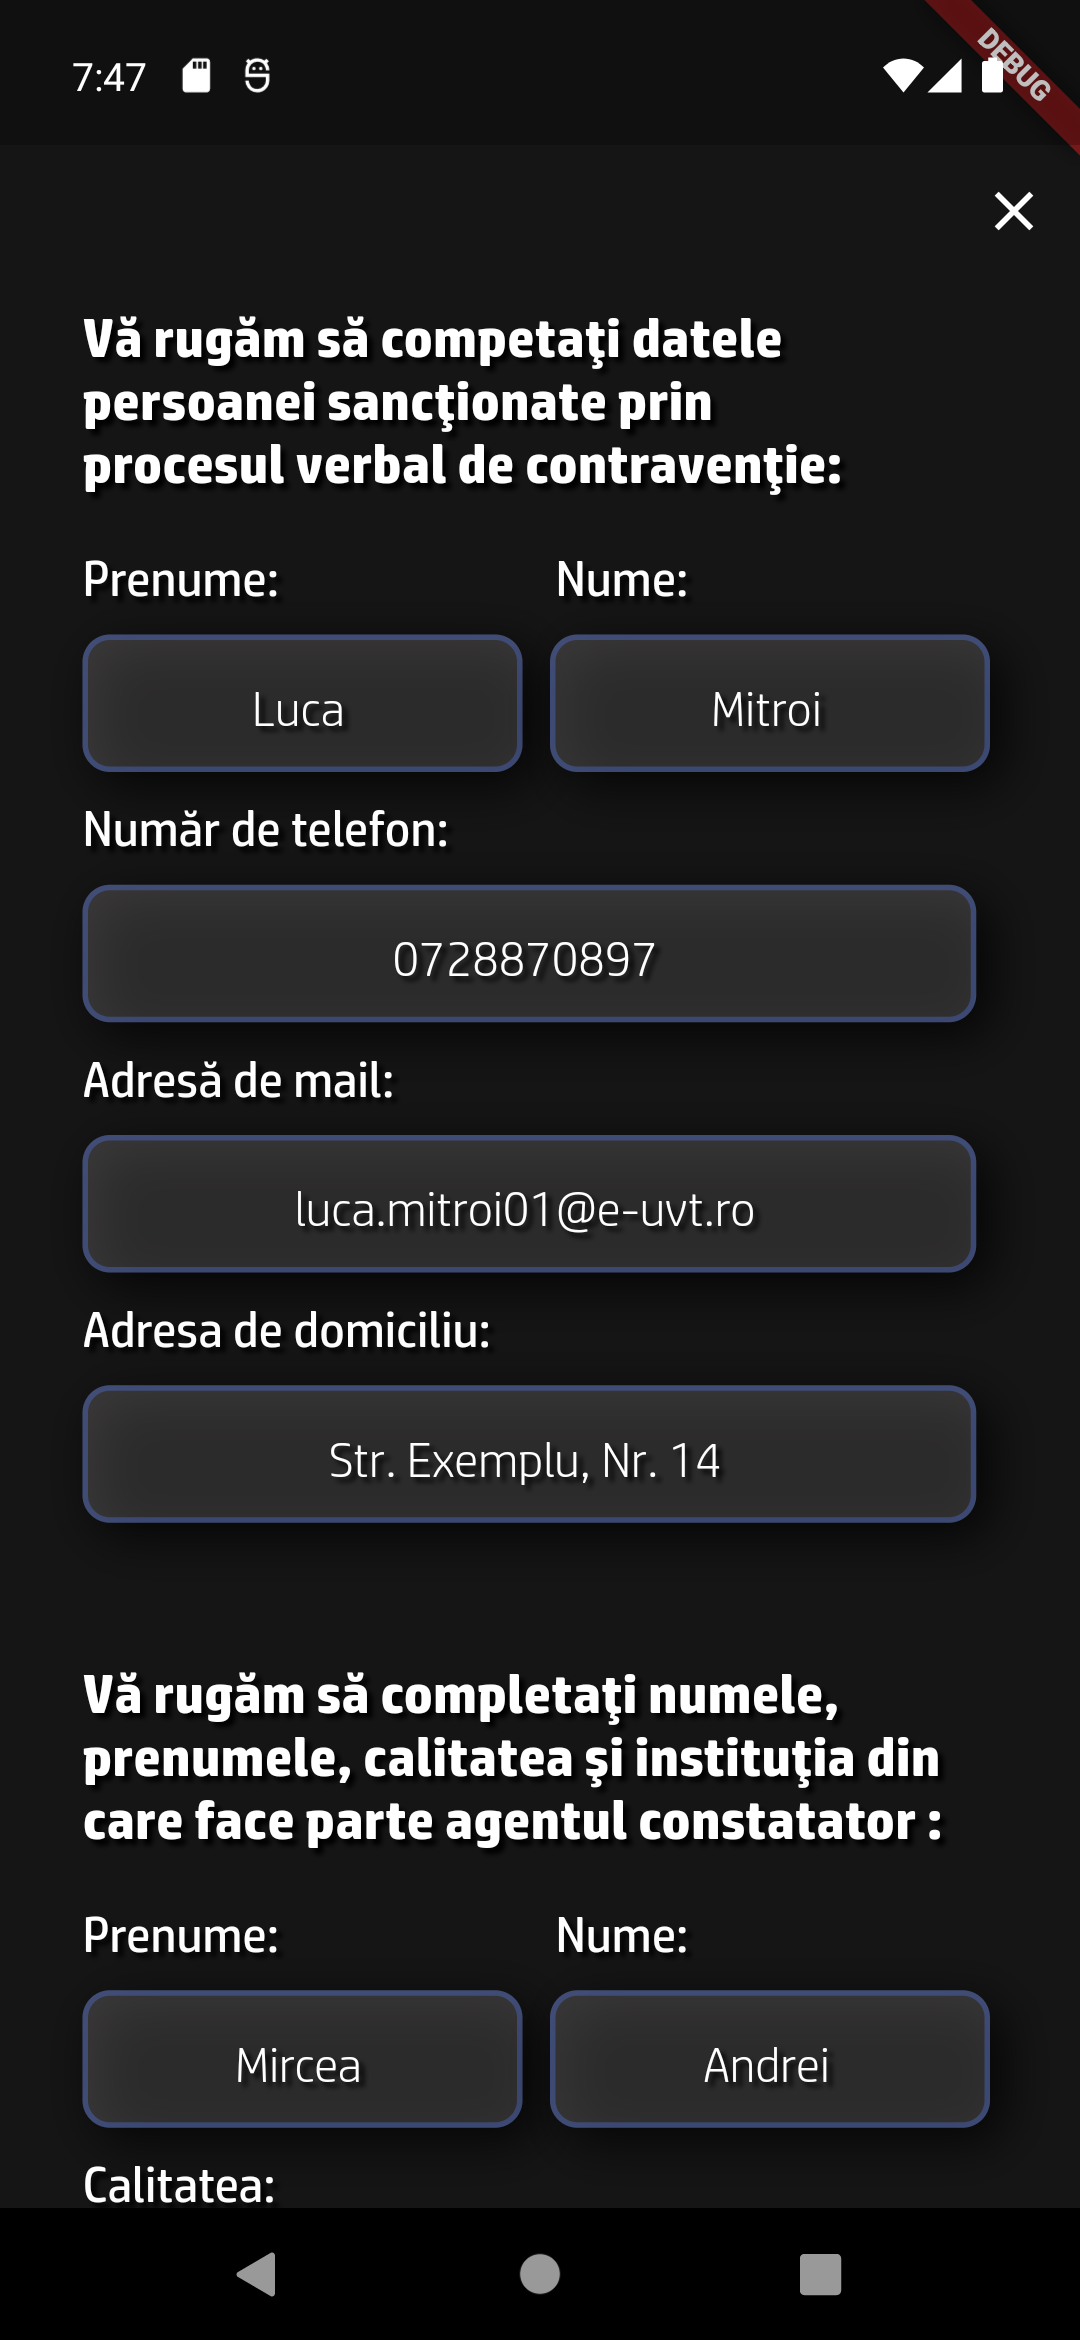
\includegraphics[width=0.25\textwidth]{images/ecran8}}
  \hspace{2.0cm}
  \subfloat[Plata prin Paypal]{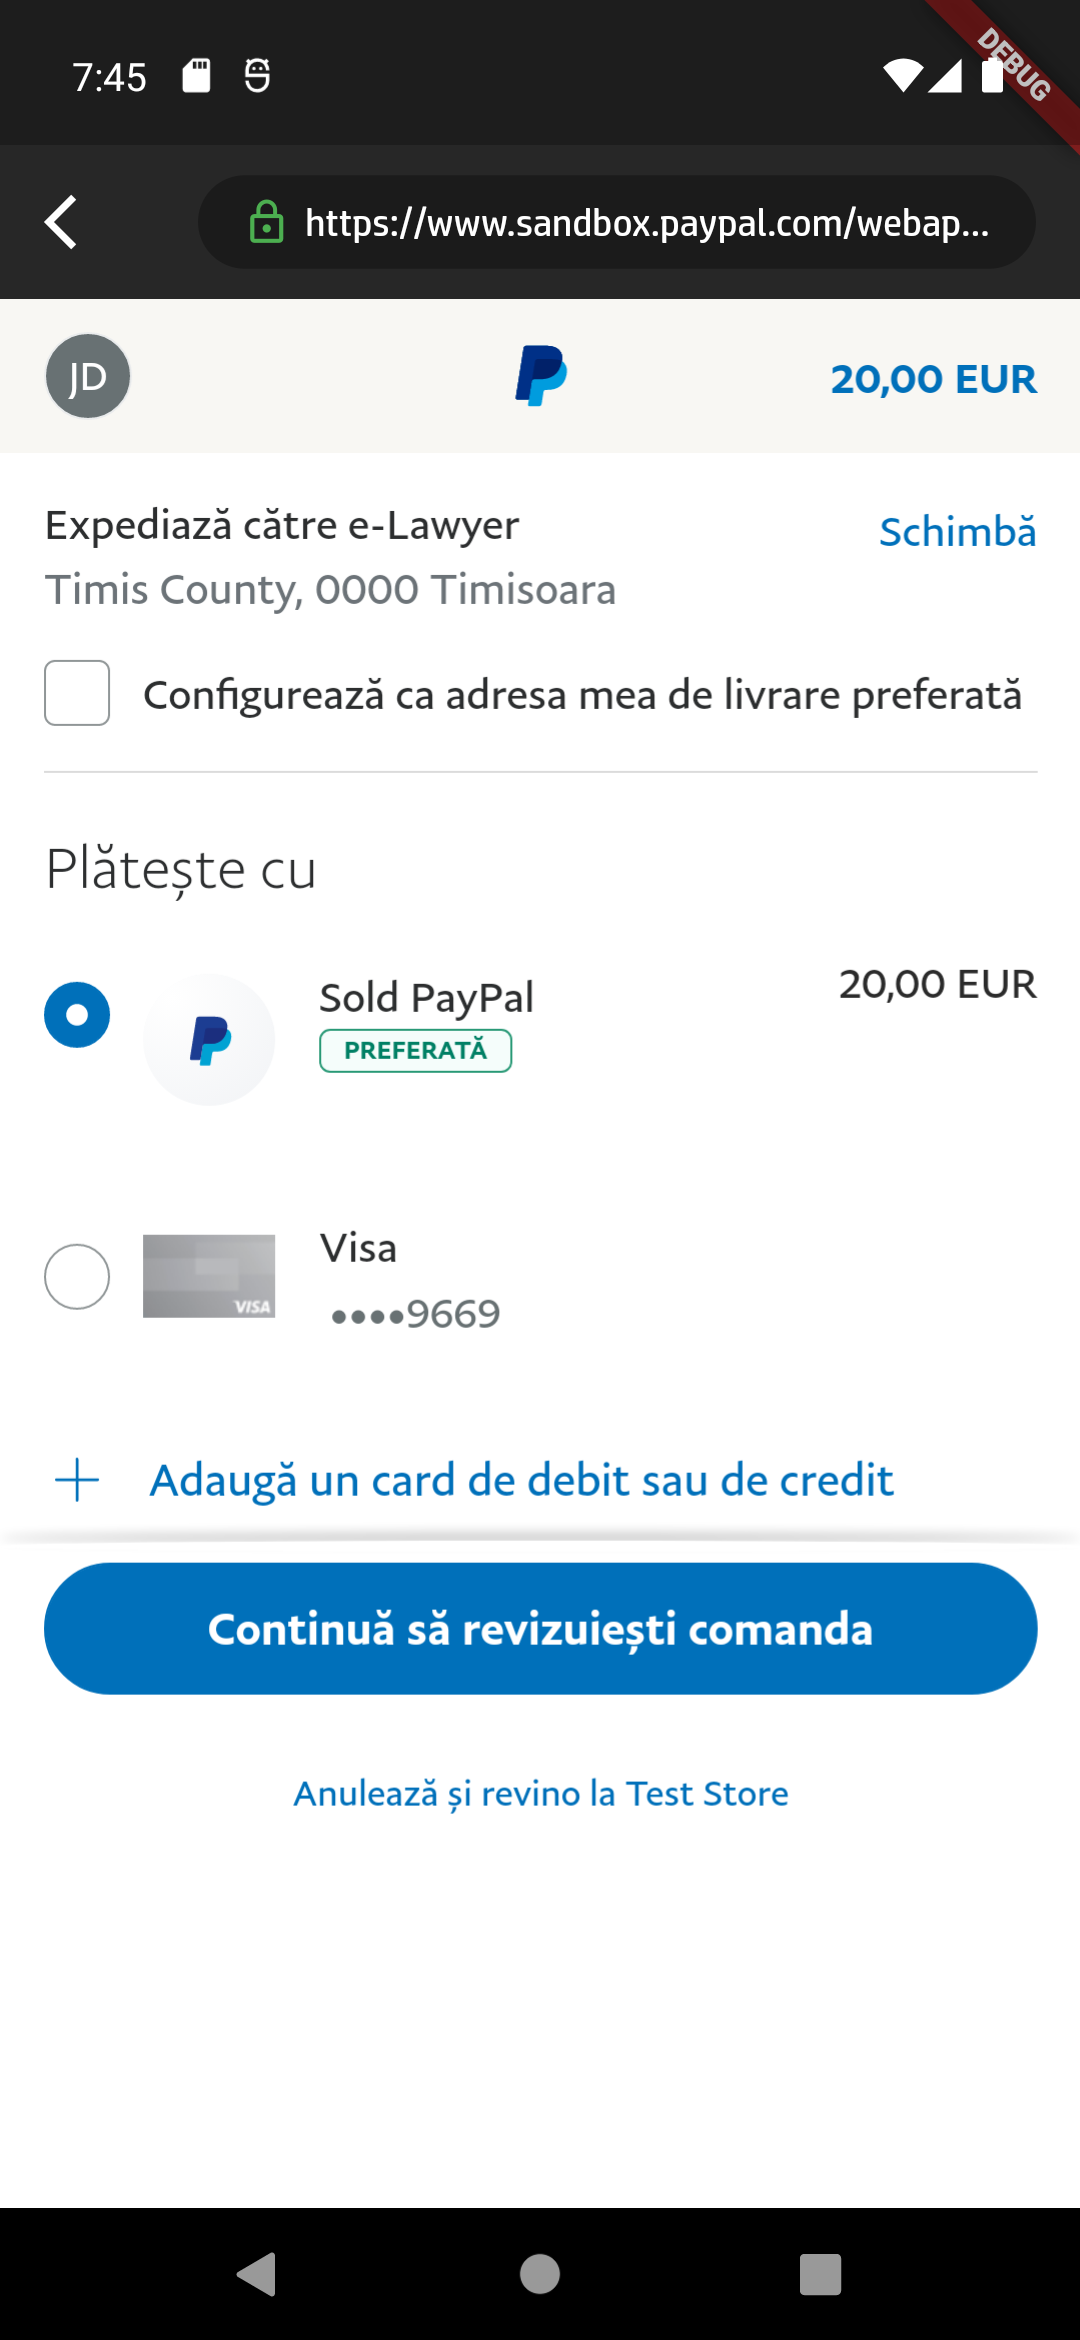
\includegraphics[width=0.25\textwidth]{images/paypal}\label{fig:f2}}
  \caption{Interfața grafică utilizată în editarea plângerilor, respectiv plătirea serviciului prin PayPal}
\end{figure}
 Aici se pot edita majoritatea informațiilor introduse, pentru ca utilizatorul să poată să se asigure că toate informațiile ajung în mod corect la avocat. După ce au fost modificate toate datele introduse inițial în mod eronat, utilizatorul poate să apese pe butonul denumit "Modificare" pentru a salva datele editate. O altă opțiune pe care o are utilizatorul în cadrul acestui ecran este opțiunea de a șterge această plângere, în cazul în care consideră că dorește să ia de la început tot procesul. Această opțiune dispare în momentul în care plângerea este plătită. 
 
Al doilea buton prezent în cadrul unei plângeri este acela de plată al serviciului. În momentul în care utilizatorul apasă acest buton, este redirecționat către o pagină de Paypal în cadrul căreia este afișat prețul cerut și metoda de plată pe care utilizatorul dorește să o folosească. Prețul afișat poate să varieze în funcție de tipul de plângere pe care utilizatorul îl selectează. Integrarea sistemului de plată a fost realizată prin intermediul API-ului oferit de către cei de la Paypal. Aplicația trimite detaliile legate de produsul vândut, aceste detalii fiind ulterior afișate la momentul realizării plății. După ce plata a fost realizată, Paypal trimite înapoi un răspuns în funcție de gradul de succes al plății, iar în funcție de răspunsul primit este modificat statusul de plătit sau neplătit al unei plângeri. Dacă plata a fost realizată cu succes, utilizatorul este informat de acest lucru printr-un ecran în care este pus un mesaj sugestiv, iar plângerea este mutată din categoria de plângeri neplătite în cea de plângeri plătite. 

În momentul în care o plângere este mutată în categoria plângerilor plătite aceasta devine vizibilă în interfața contului de avocat. Tot ce mai poate utilizatorul în acest moment este să editeze datele din plângere și să aștepte un răspuns de la avocat. Acesta poate să fie "Aprobată" sau "Respinsă". În cazul în care o plângere este respinsă utilizatorul are opțiunea să o editeze în continuare pentru a actualiza datele astfel încât plângerea să fie adusă într-un stadiu în care să poată să fie aprobată. În momentul în care datele au fost editate se schimbă statusul de la "Respinsă" înapoi la "Așteptare" astfel încât avocatul să poată să se uite în continuare la datele modificate. 

În cazul în care avocatul aprobă o plângere, aceasta este trecută ca plângere aprobată în interfața utilizatorului care a creat plângerea. Astfel dispare opțiunea de a edita datele, dar această opțiune este înlocuită de cea de descărcare a PDF-ului cu produsul final. Acest PDF este salvat în fișierele dispozitivului clientului în folderul Downloads al dispozitivului. 

Ultimul element din interfața ecranului Acasă care nu a fost menționat este butonul de "Plângere nouă". Acesta este folosit pentru a crea o plângere nouă, ceea ce trimite utilizatorul în interfața creată pentru această acțiune. Acest buton dispare de pe ecran în momentul în care utilizatorul începe să dea scroll în jos pe ecran, pentru a oferi o vizualizare mai curată a celorlalte elemente vizuale de pe ecran, dar reapare în momentul în care utilizatorul dă scroll în sus. Această funcționalitate este asemănătoare cu butonul de compunere de pe aplicația Gmail care se comportă într-un mod asemănător.
\begin{center}
\begin{figure}[H]
    	\centering
    	
\includegraphics[width = 0.3\textwidth]{images/buton}
	\caption{Butonul utilizat pentru compunerea unei plângeri noi}
\end{figure}
\end{center}

\newpage
\section{Compunerea plângerii}
\vspace{20pt}
Din ecranul principal al aplicației, utilizatorul poate să acceseze principala funcție a aplicației, aceea fiind cea de a compune o plângere nouă. Acesta poate să inițieze acest lucru apăsând pe butonul \textbf{"Contestație nouă"}. Butonul este localizat în partea inferioară a ecranului, în dreapta. Datele pe care utilizatorul trebuie să le introducă sunt împărțite în mai multe câmpuri dintr-un formular, care sunt ușor de urmărit. Unele câmpuri sunt câmpuri de tip text, în care utilizatorul trebuie să introducă datele corespunzătoare cu textul de deasupra câmpului. Uneori în aceste câmpuri trebuie introdusă informație numerică, astfel că tastatura dispozitivului afișează doar caracterele corecte care pot fi introduse. În alte cazuri, utilizatorul trebuie să introducă informații de tip dată. În momentul în care apasă pe câmpul cu acest tip de dată, aplicația afișează un meniu de tip calendar pentru a ușura această selecție. 

Alte elemente prezente în acest formular sunt butoanele de tip DA/NU. Aceste butoane au două opțiuni, iar utilizatorul trebuie să o aleagă pe cea care se potrivește cu datele sale. În mod implicit, varianta NU este selectată. În cazul în care utilizatorul consideră că nu a ales opțiunea corectă are mereu varianta să editeze aceste date, ele rămânând salvate în poziția în care acesta le-a lăsat. Una din cele mai importante câmpuri este unul de acest tip (DA/NU) deoarece este selecția legată de reprezentarea în instanță a avocatului, deoarece decide ce tip de plângere este, precum și prețul final pe care utilizatorul trebuie să îl plătească.
\begin{figure}[H]
  \centering
  \subfloat[Interfața grafică a formularului]{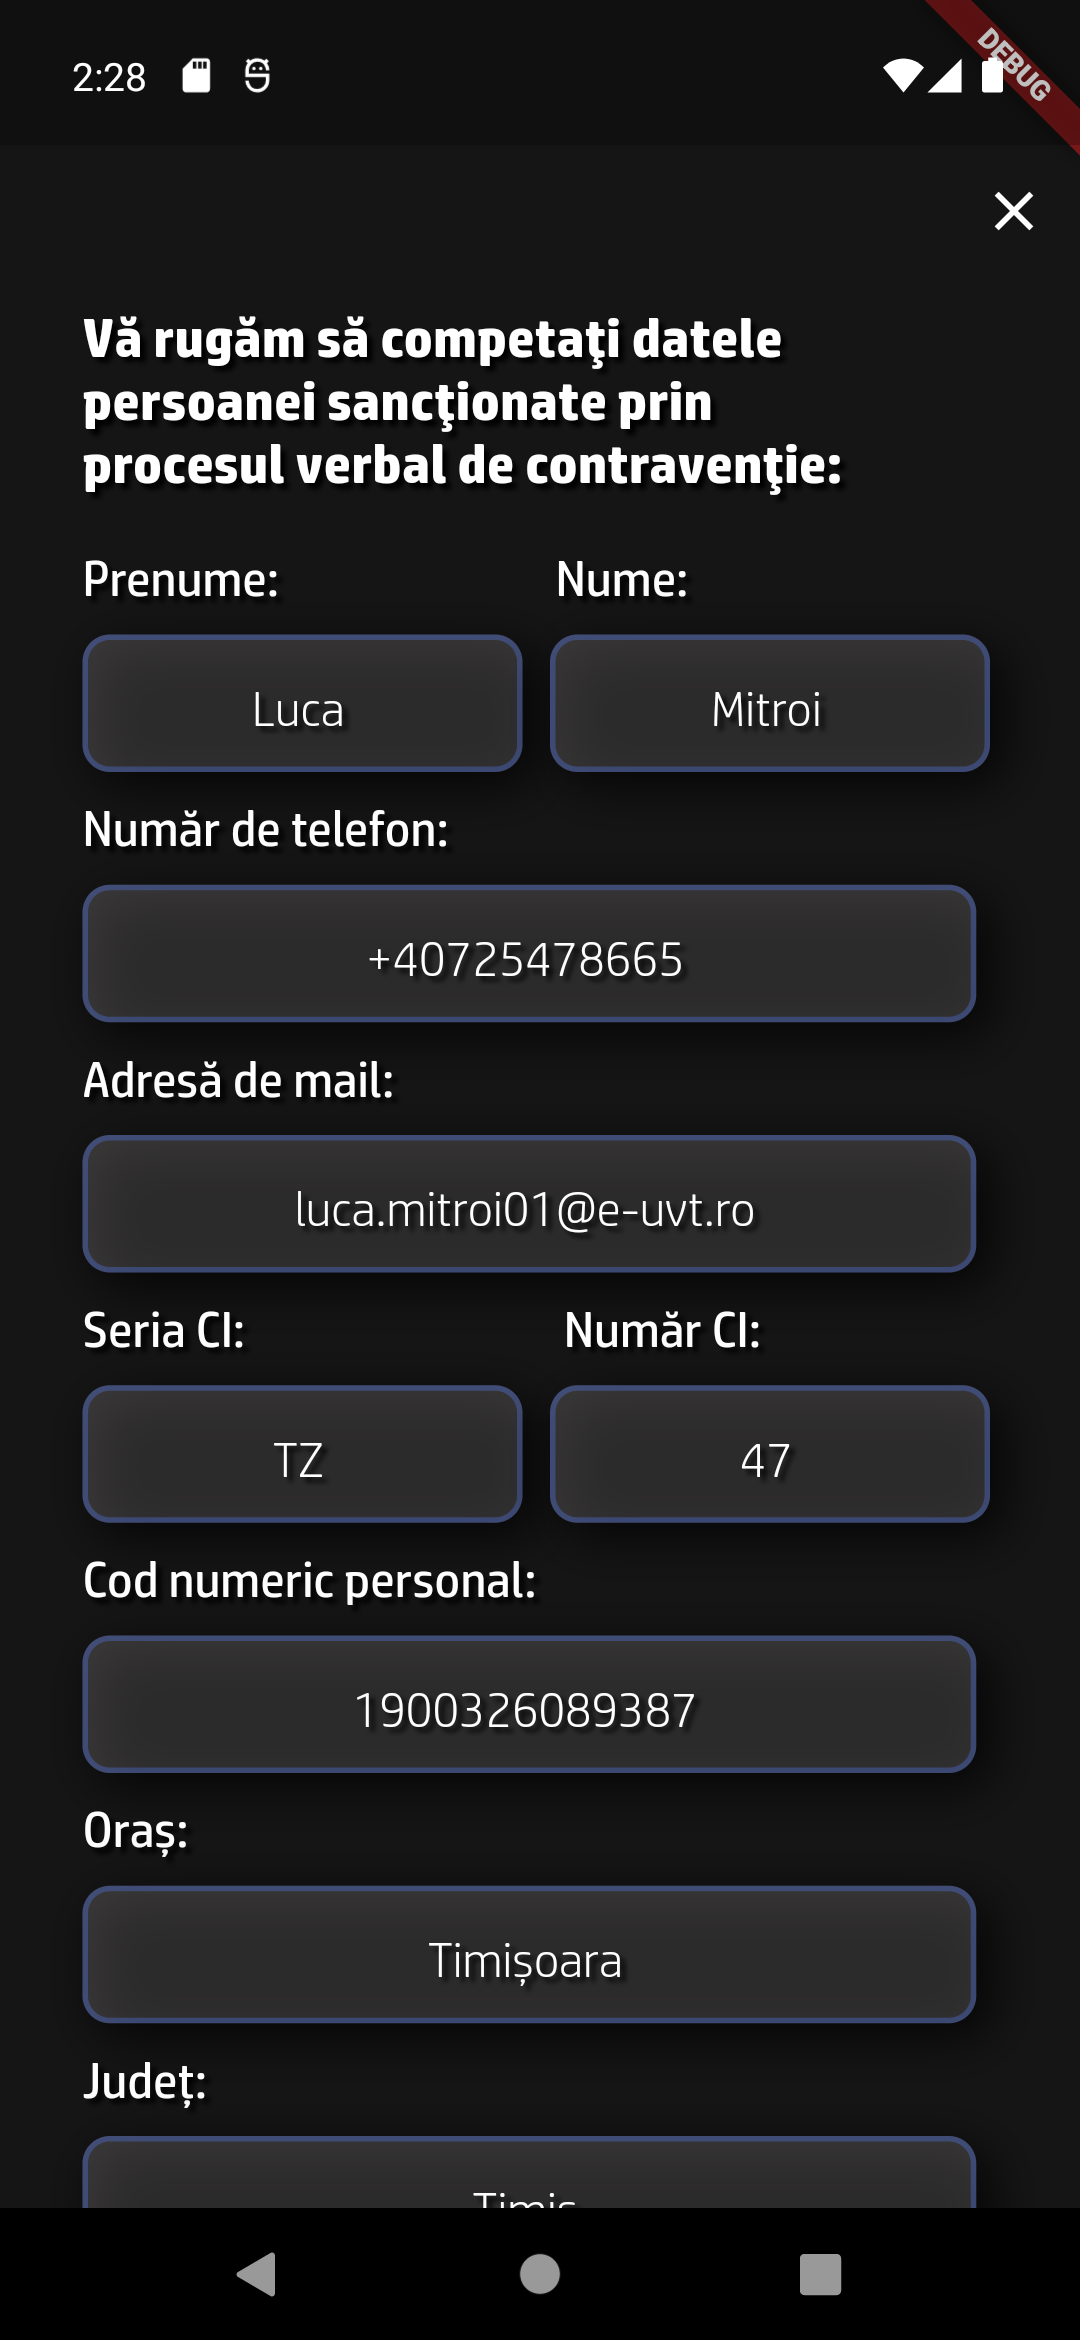
\includegraphics[width=0.3\textwidth]{images/ecran9}}
  \hspace{2.0cm}
  \subfloat[Meniul de selectare a datei]{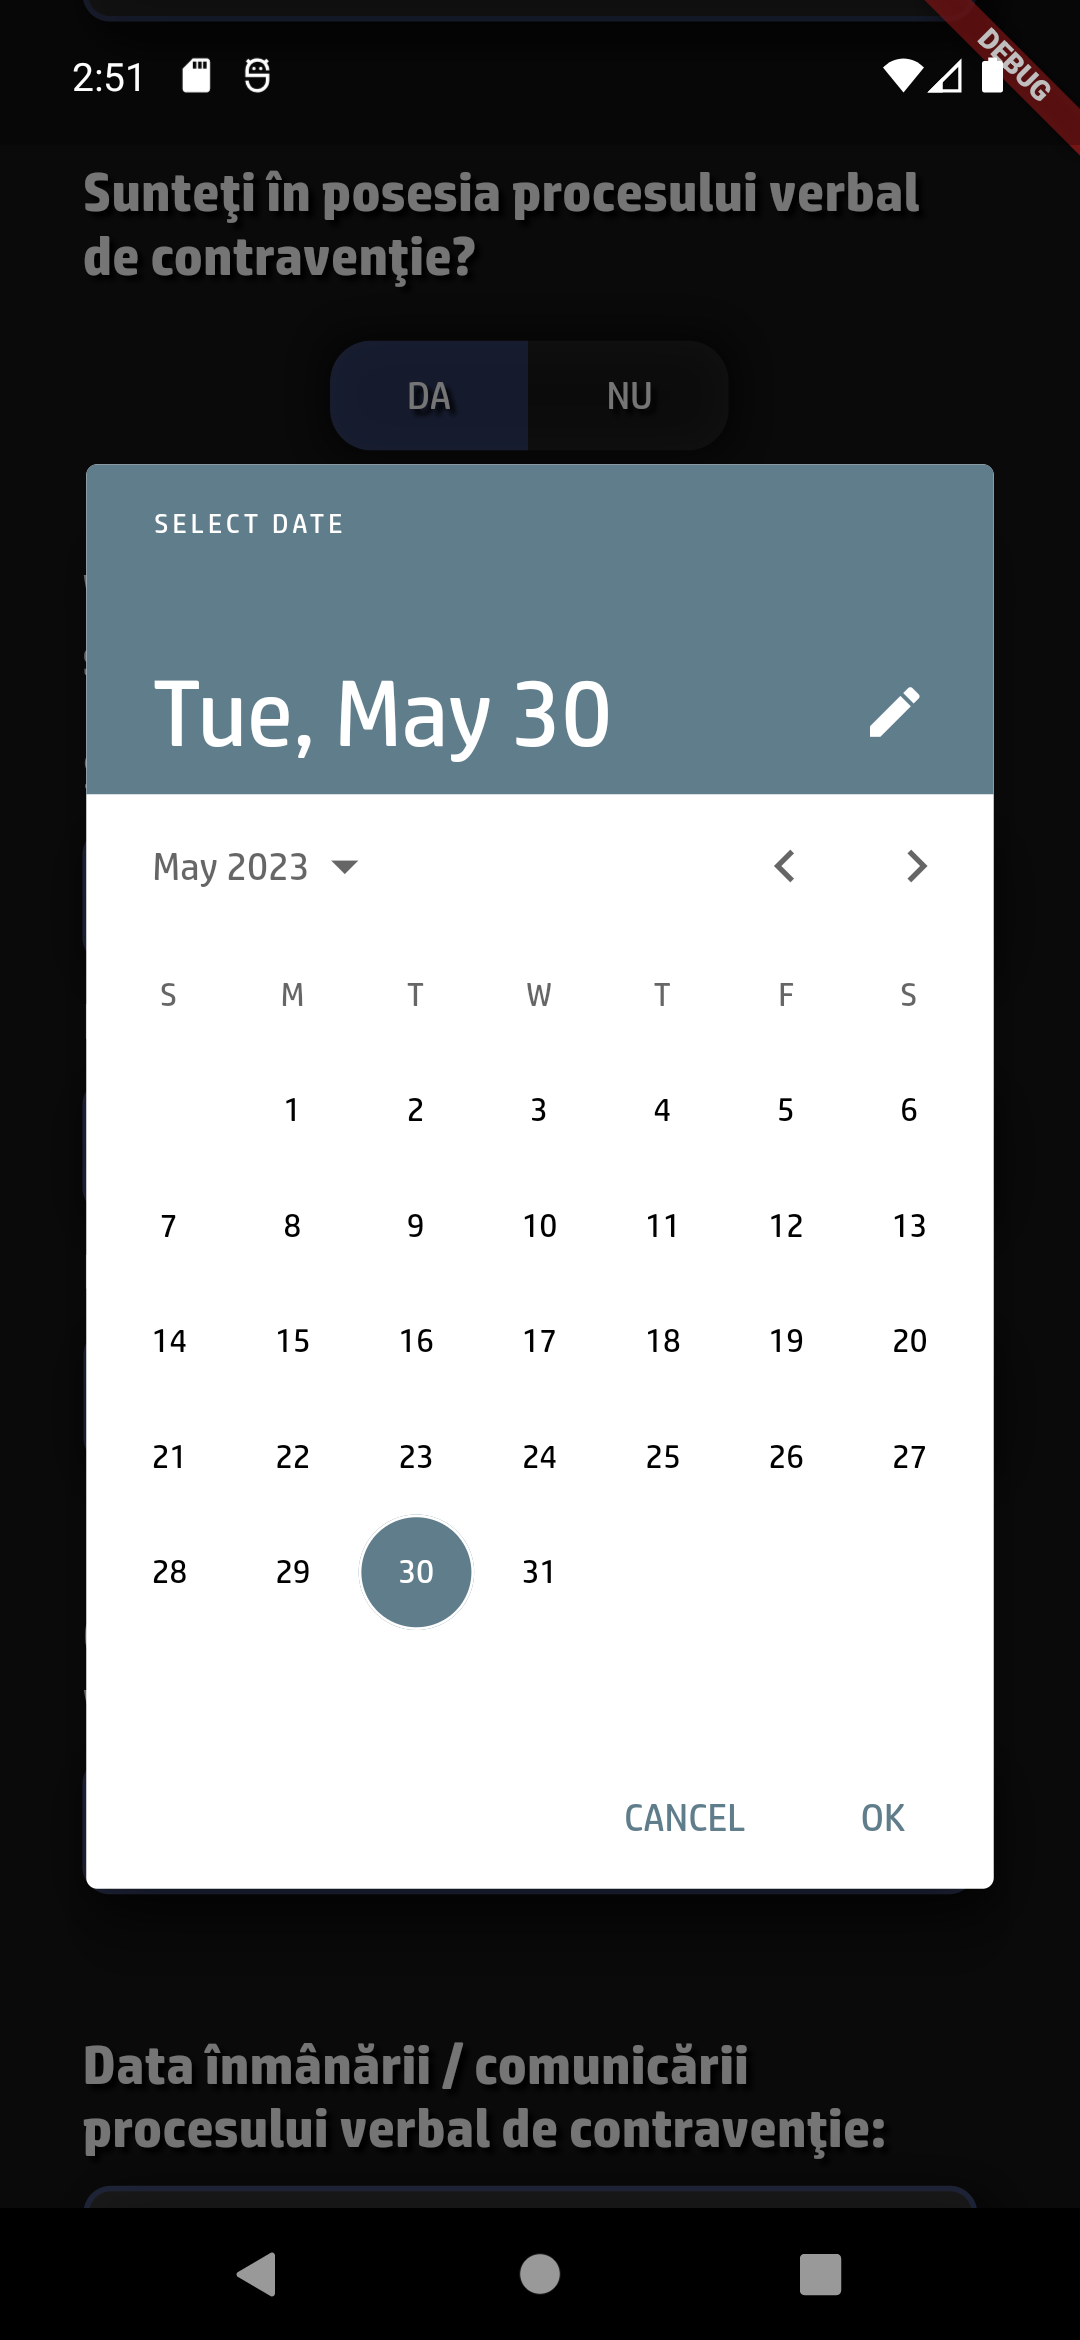
\includegraphics[width=0.3\textwidth]{images/ecran10}\label{fig:f2}}
  \caption{Ecrane din cadrul formularului de compunere a unei plângeri noi}
\end{figure}
\newpage
Una din secțiunile prezente în acest formular este cea legată de datele agentului constatator care a emis amenda. În cadrul acestor informații se regăsește și o secțiune în care utilizatorul trebuie să introducă numele și adresa secției din cadrul căreia agentul constatator face parte. Pentru ușurarea introducerii acestor date, a fost introdus în cadrul aplicației un fișier JSON care conține datele esențiale a unui număr mare de secții din cadrul țării. Pe baza acestui fișier, au fost realizate mai multe liste în cadrul interfeței grafice, din care utilizatorul poate să aleagă opțiunile care se potrivesc cu cazul acestuia. Opțiunile din fiecare listă se actualizează în funcție de ce a ales utilizatorul anterior. De exemplu, dacă utilizatorul alege un județ anume, se actualizează lista cu orașele în funcție de județul ales și așa mai departe. În cazul în care totuși opțiunea pe care utilizatorul vrea să o introducă nu există în acest fișier JSON, acesta are și opțiunea să introducă o informație proprie. Au fost realizate și câteva mecanisme de siguranță în aceste câmpuri. De exemplu, în cazul în care se modifică opțiunea aleasă la o listă anterioară, toate câmpurile următoare din această secțiune sunt golite pentru a asigura corectitudinea datelor.

În momentul în care utilizatorul a completat toate câmpurile și a bifat câmpul legat de colectarea datelor în conformitate cu GDPR acesta trebuie să apese pe butonul Submit. În momentul în care acest buton este apăsat, aplicația verifică dacă toate câmpurile sunt completate, deoarece toate sunt obligatorii. În caz contrar, aplicația trimite un popup care să avertizeze utilizatorul de faptul că nu sunt satisfăcute toate cerințele necesare pentru încărcarea datelor și crearea unei plângeri noi. 

În cazul în care toate cerințele sunt satisfăcute, aplicația trimite un mesaj de succes care informează utilizatorul că încărcarea a fost realizată cu succes, ulterior acesta fiind redirecționat către ecranul principal unde apar datele introduse. Datele sunt încărcate în baza de date prin intermediul apelului POST realizat prin intermediul REST API. Plângerea este stocată ca un element dintr-un fișier JSON care este asociat userului creator prin intermediul id-ului acesta. 

\begin{figure}[H]
  \centering
  \subfloat{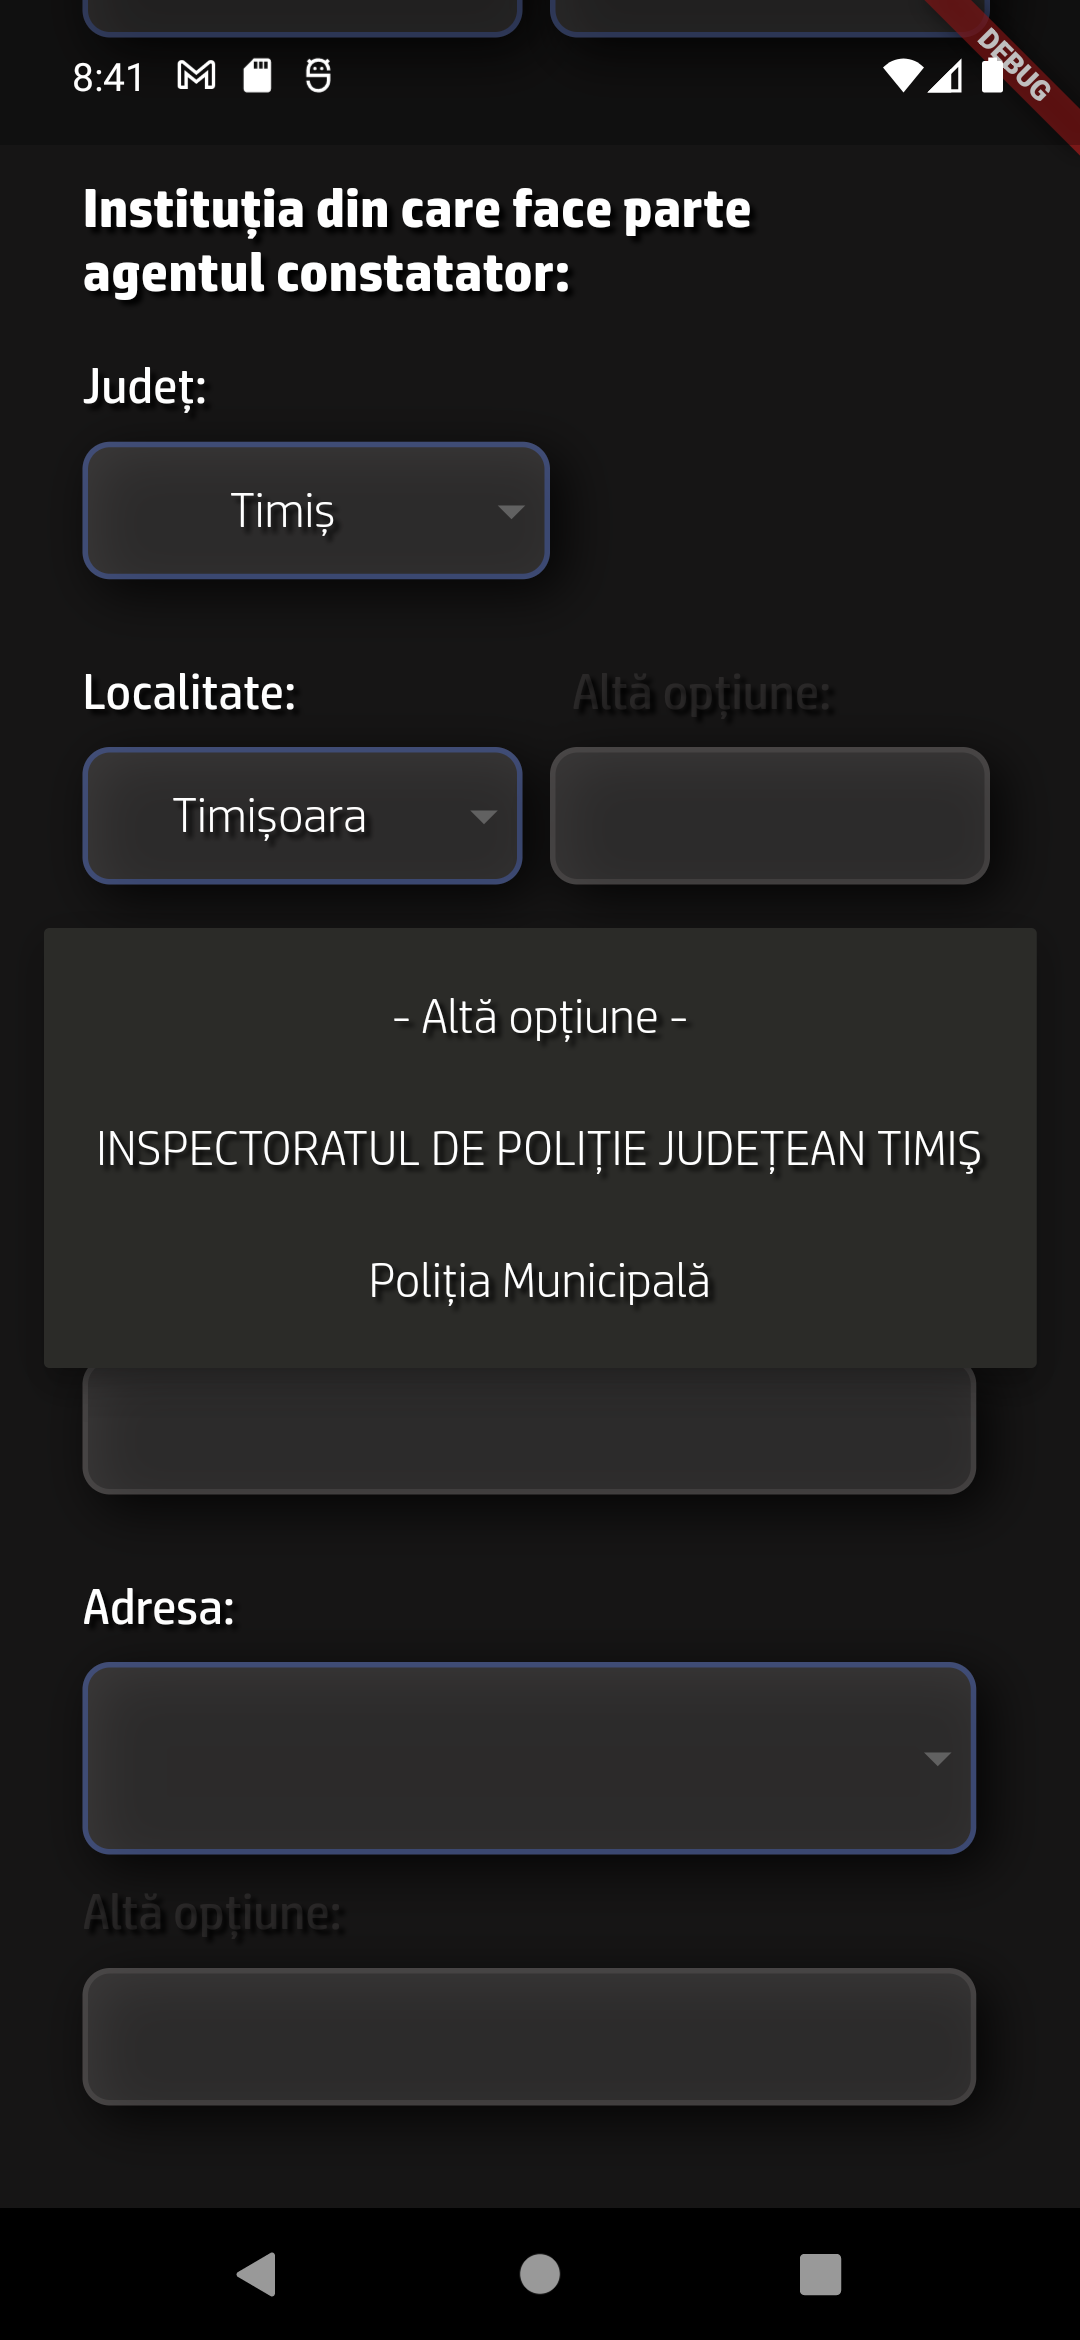
\includegraphics[width=0.25\textwidth]{images/ecran16}}
  \hspace{2.0cm}
  \subfloat{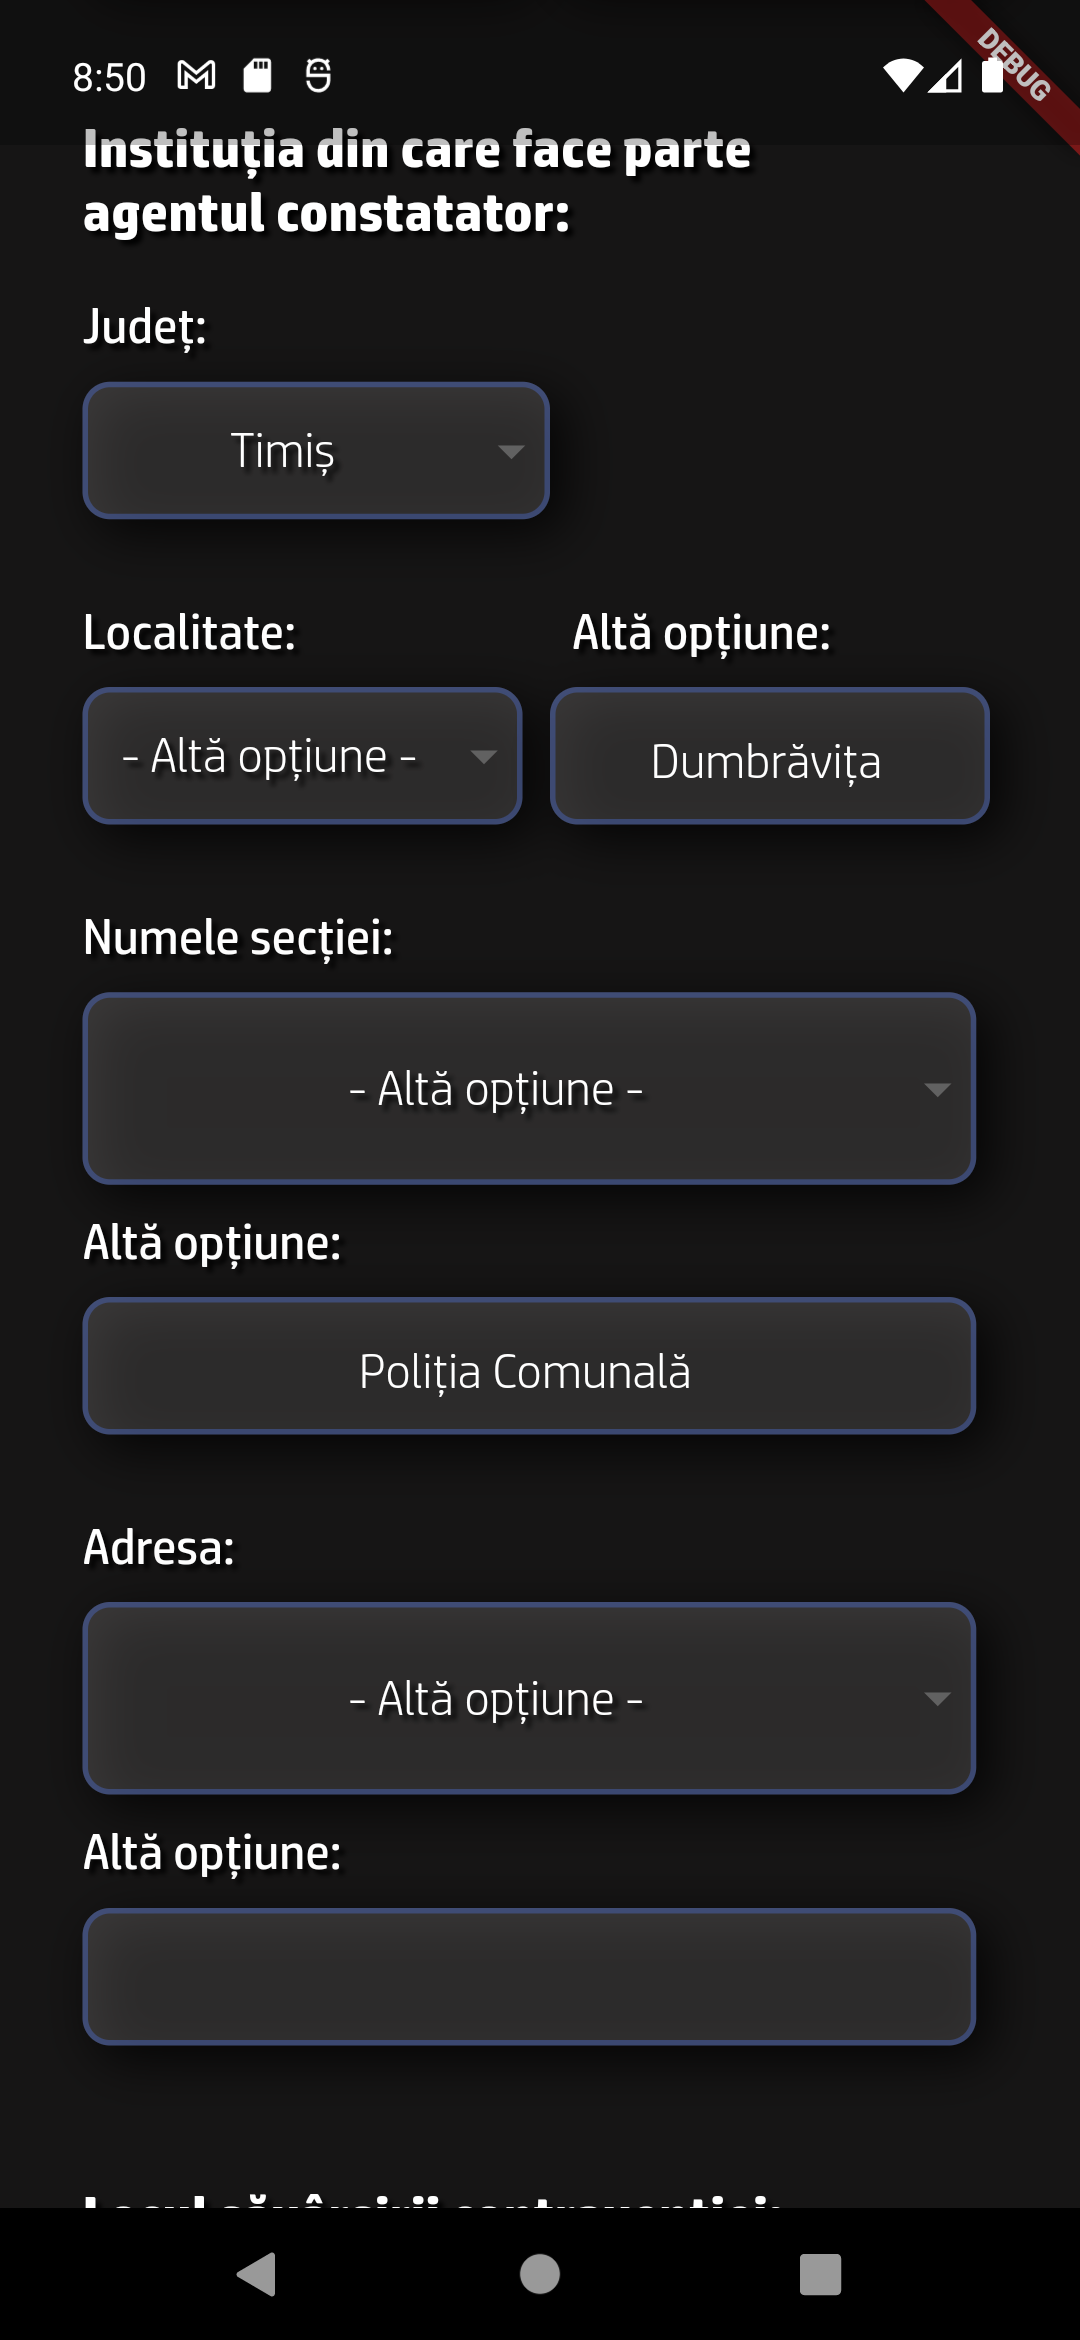
\includegraphics[width=0.25\textwidth]{images/ecran17}}
  \caption{Câmpurile în care se introduc datele legate de secția de poliție din care face parte agentul constatator}
\end{figure}

\newpage
\section{Contul utilizatorilor de tip avocat}
\vspace{20pt}
Un alt aspect important al aplicației este reprezentat de rolul avocaților în cadrul acestei aplicații. Aceștia au o categoria specială de conturi, deoarece au atribuții diferite față de utilizatorii normali precum și alte responsabilități. În momentul de față modul în care este creat un astfel de cont este doar direct prin contactarea deținătorilor aplicației deoarece doar aceștia pot să creeze conturi de tip avocat. Acestă decizie este motivată de faptul că este necesară o verificare în detaliu asupra actelor doveditoare care atestă calitatea de avocat a persoanei care dorește să își creeze contul.

După ce acest cont a fost creat, logarea se realizează în același mod precum restul conturilor: prin adresa de mail și prin parolă. Interfața care a fost realizată pentru conturile de avocat este asemănătoare cu cea a conturilor de client, însă există câteva diferențe notabile. În primul rând, în bara de navigare există doar două opțiuni (față de trei pentru conturile de client), acestea fiind: Acasă și Profil. Utilizatorii de tip avocat își pot modifica datele legate de contul de utilizator în același mod în care o pot face și utilizatorii de tip client.

În secțiunea Acasă sunt prezente toate plângerile de la toți utilizatorii. Acestea sunt împărțite în două secțiuni diferite, acestea fiind \textbf{Plângeri nefinalizate} și \textbf{Plângeri finalizate}. În cadrul plângerilor nefinalizate sunt prezente plângerile care nu au primit un răspuns final, ele fiind încă în stadiul de "În așteptare". Acestea au prezente patru opțiuni pe care avocatul poate să le folosească: Editare, Descarcă PDF, Respingere și Aprobare. Pentru ca un avocat să poată să vizualizeze stadiul în care se află o plângere nefinalizată are două opțiuni: fie să descarce direct PDF-ul care este generat în aplicație, în care au fost introduse datele pe care le-a scris utilizatorul, fie să apese pe butonul Editare, în care sunt dispuse detaliile într-un format tabelar, asemănător cu cel din cadrul creării unei plângeri.

Avocatului îi sunt prezentate date de identificare legate de utilizatorul care a creat o plângere. Aceste date sunt trecute deoarece avocatul poate să comunice prin intermediu mail-ului cu un utilizator în cazul în care există neclarități, sau erori în cadrul datelor trimise de către acesta. Principala atribuție pe care o are un avocat în cadrul acestei aplicații este să verifice corectitudinea informațiilor primite de la un client pentru a se asigura că produsul final (PDF-ul generat) este cât mai corect și are o șansă cât mai mare să câștige cazul clientului. În cazul în care avocatul ajunge la un consens împreună cu clientul contactat, acesta are opțiunea de a modifica datele din cadrul plângerii. Interfața de editare este asemănătoare cu cea disponibilă în cadrul conturilor de utilizator astfel că avocatul poate să modifice toate câmpurile. Singura diferență este legată de faptul că avocatul nu are posibilitatea să șteargă o plângere a unui utilizator, deoarece aceasta a fost plătită.

După ce au fost realizate toate verificările necesare, avocatul trebuie să ajungă la o concluzie în legătură cu plângerea. Acesta are două opțiuni: Aprobare sau Respingere. În momentul în care avocatul apasă unul din cele două butoane de pe interfață, un mail este trimis către utilizatorul care a inițial cererea de creare de plângere. Acest mail informează utilizatorul în legătură cu decizia pe care a luat-o avocatul, dar și titlul plângerii, pentru a putea identifica cu ușurință despre care plângere este vorba în cazul în care există mai multe plângeri în prelucrare.
\newpage
\section{Funcționalități adiționale}
În cadrul aplicației mai există câteva funcționalități adiționale care nu au fost descrise până acum. Acestea se găsesc în ecranul Meniu, acesta fiind disponibil în bara de navigare localizată în partea inferioară a ecranului. Acest meniu este prezent doar la conturile de client, deoarece sunt funcții care ajută clientul, nu atât avocatul. Aceste funcționalități sunt reprezentate de butoanele \textbf{"Locații utile"}, \textbf{"Informații legale"} și \textbf{"Informații aplicație"}.

Secțiunea \textbf{"Locații utile"} redirecționează utilizatorul către o hartă în care sunt evidențiate locațiile cu secțiile de poliție care se află în proximitate cu utilizatorul. Acest lucru este realizat prin redirecționarea către Google Maps, într-o fereastră de Browser integrată în aplicație. Singura cerință necesară pentru a putea fi folosită această funcționalitate a aplicației este ca utilizatorul să fie conectat la contul său de Google, însă în cele mai multe cazuri utilizatorul deja are un cont de Google asociat telefonului deoarece este o componentă foarte importantă a sistemului de operare Android. Integrarea Browserului este realizată prin intermediul pachetului url\_launcher oferit de către Flutter.

Secțiunea \textbf{"Informații legale"} redirecționează utilizatorul către o pagină Web în care se află întreg codul rutier. Este destul de util ca un utilizator să aibă acces la codul rutier într-un mod cât mai simplu și la îndemână, deoarece este important ca în momentul în care sunt introduse datele despre amendă, precum și perspectiva proprie asupra evenimentelor, ca utilizatorul să cunoască toate informațiile legale, iar un acces foarte rapid la codul rutier ajută mult cu acest aspect. 

Secțiunea \textbf{"Informații aplicație"} redirecționează utilizatorul către un ecran în care sunt expuse anumite informații utile despre aplicație. Aici sunt explicate întrebări probabile pe care ar putea utilizatorul să le aibă precum cum se realizează comunicarea cu avocatul, sau cum se realizează plata plângerilor.

\begin{figure}[H]
  \centering
  \subfloat[Meniul cu toate opțiunile adiționale]{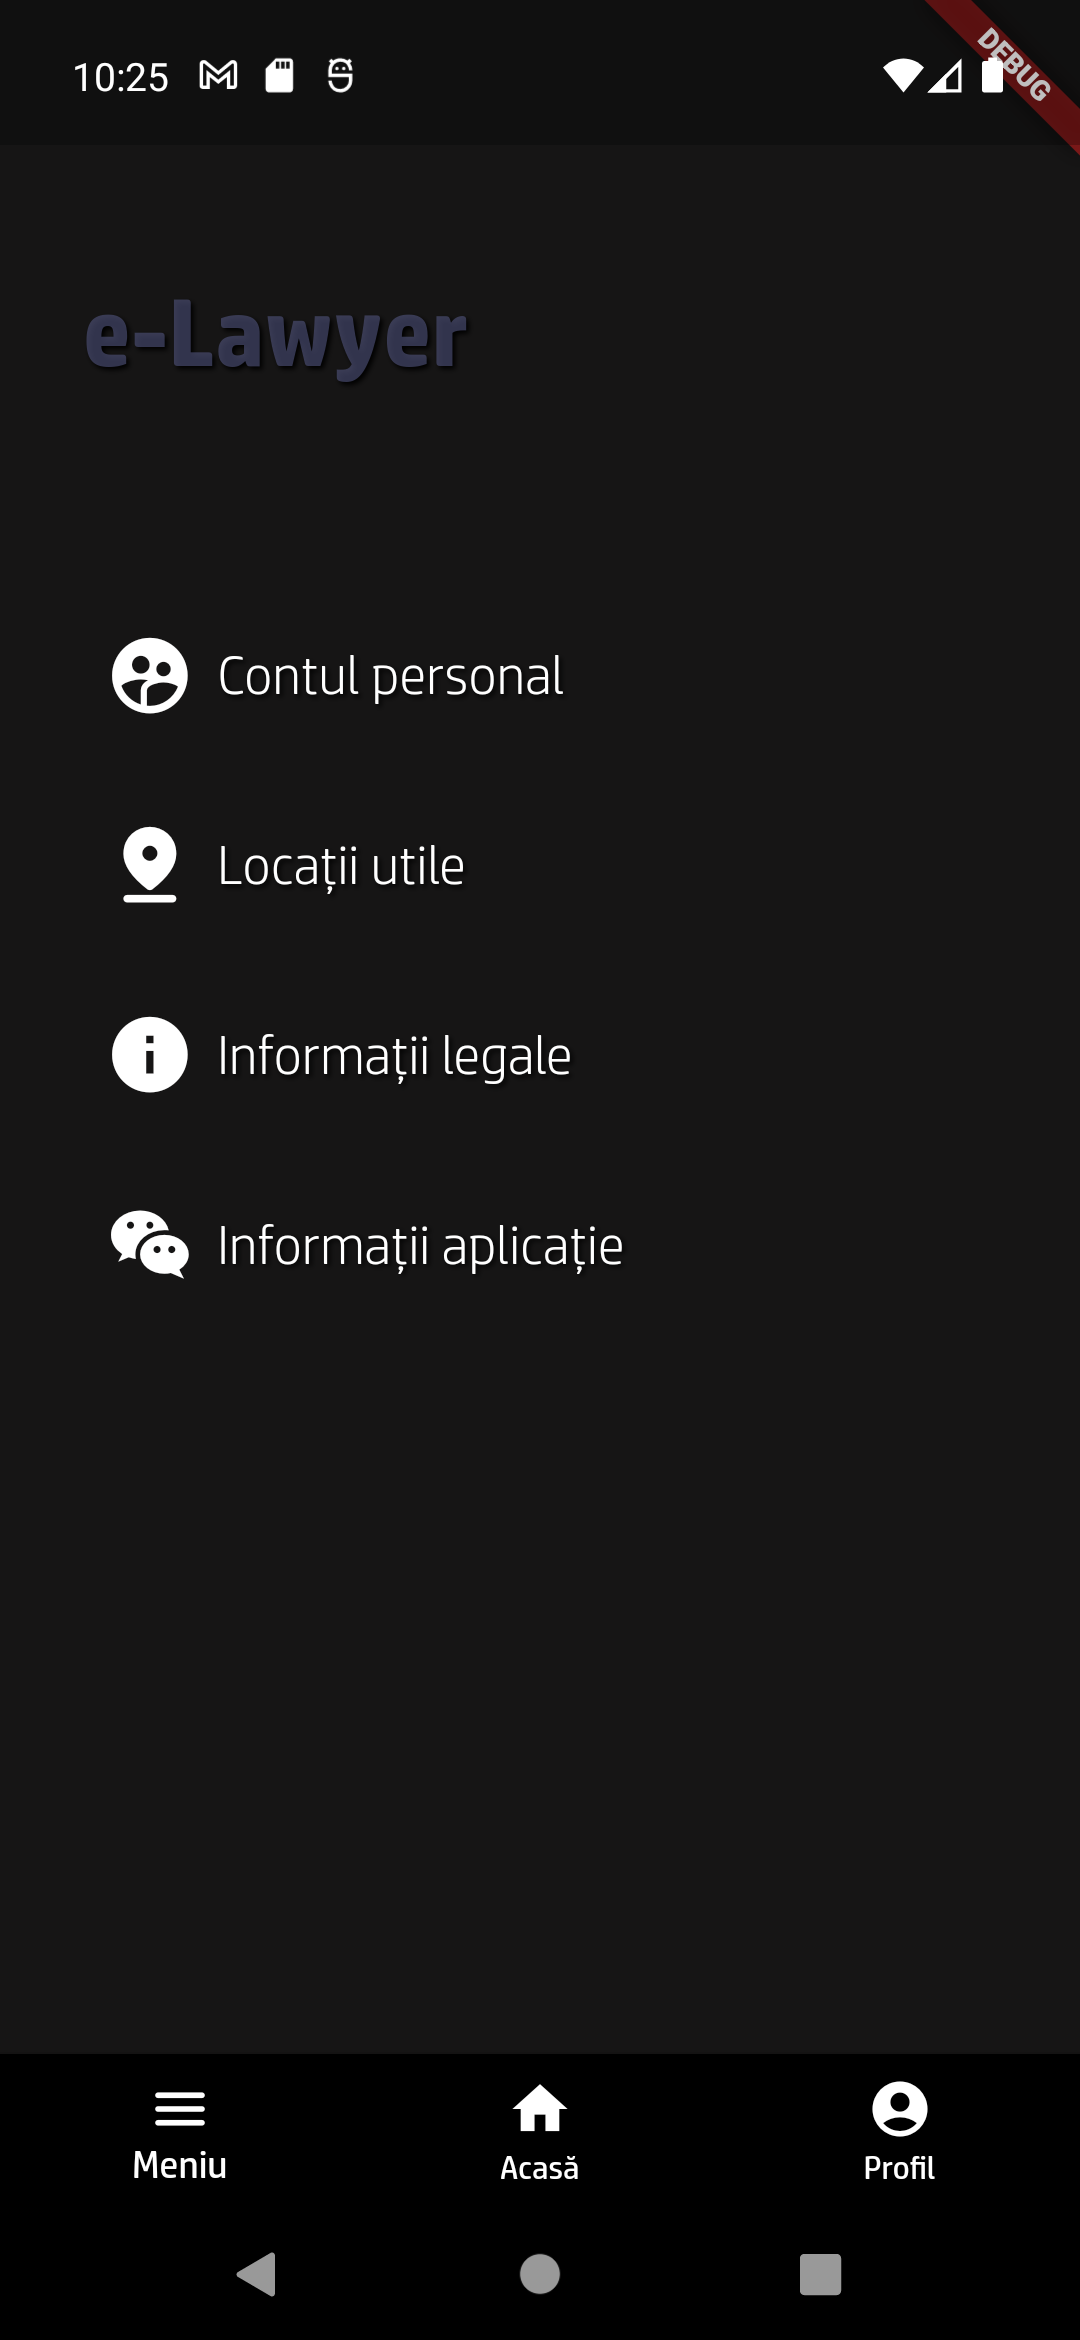
\includegraphics[width=0.23\textwidth]{images/ecran11}}
  \hspace{0.3cm}
  \subfloat[Ecranul Informații aplicație]{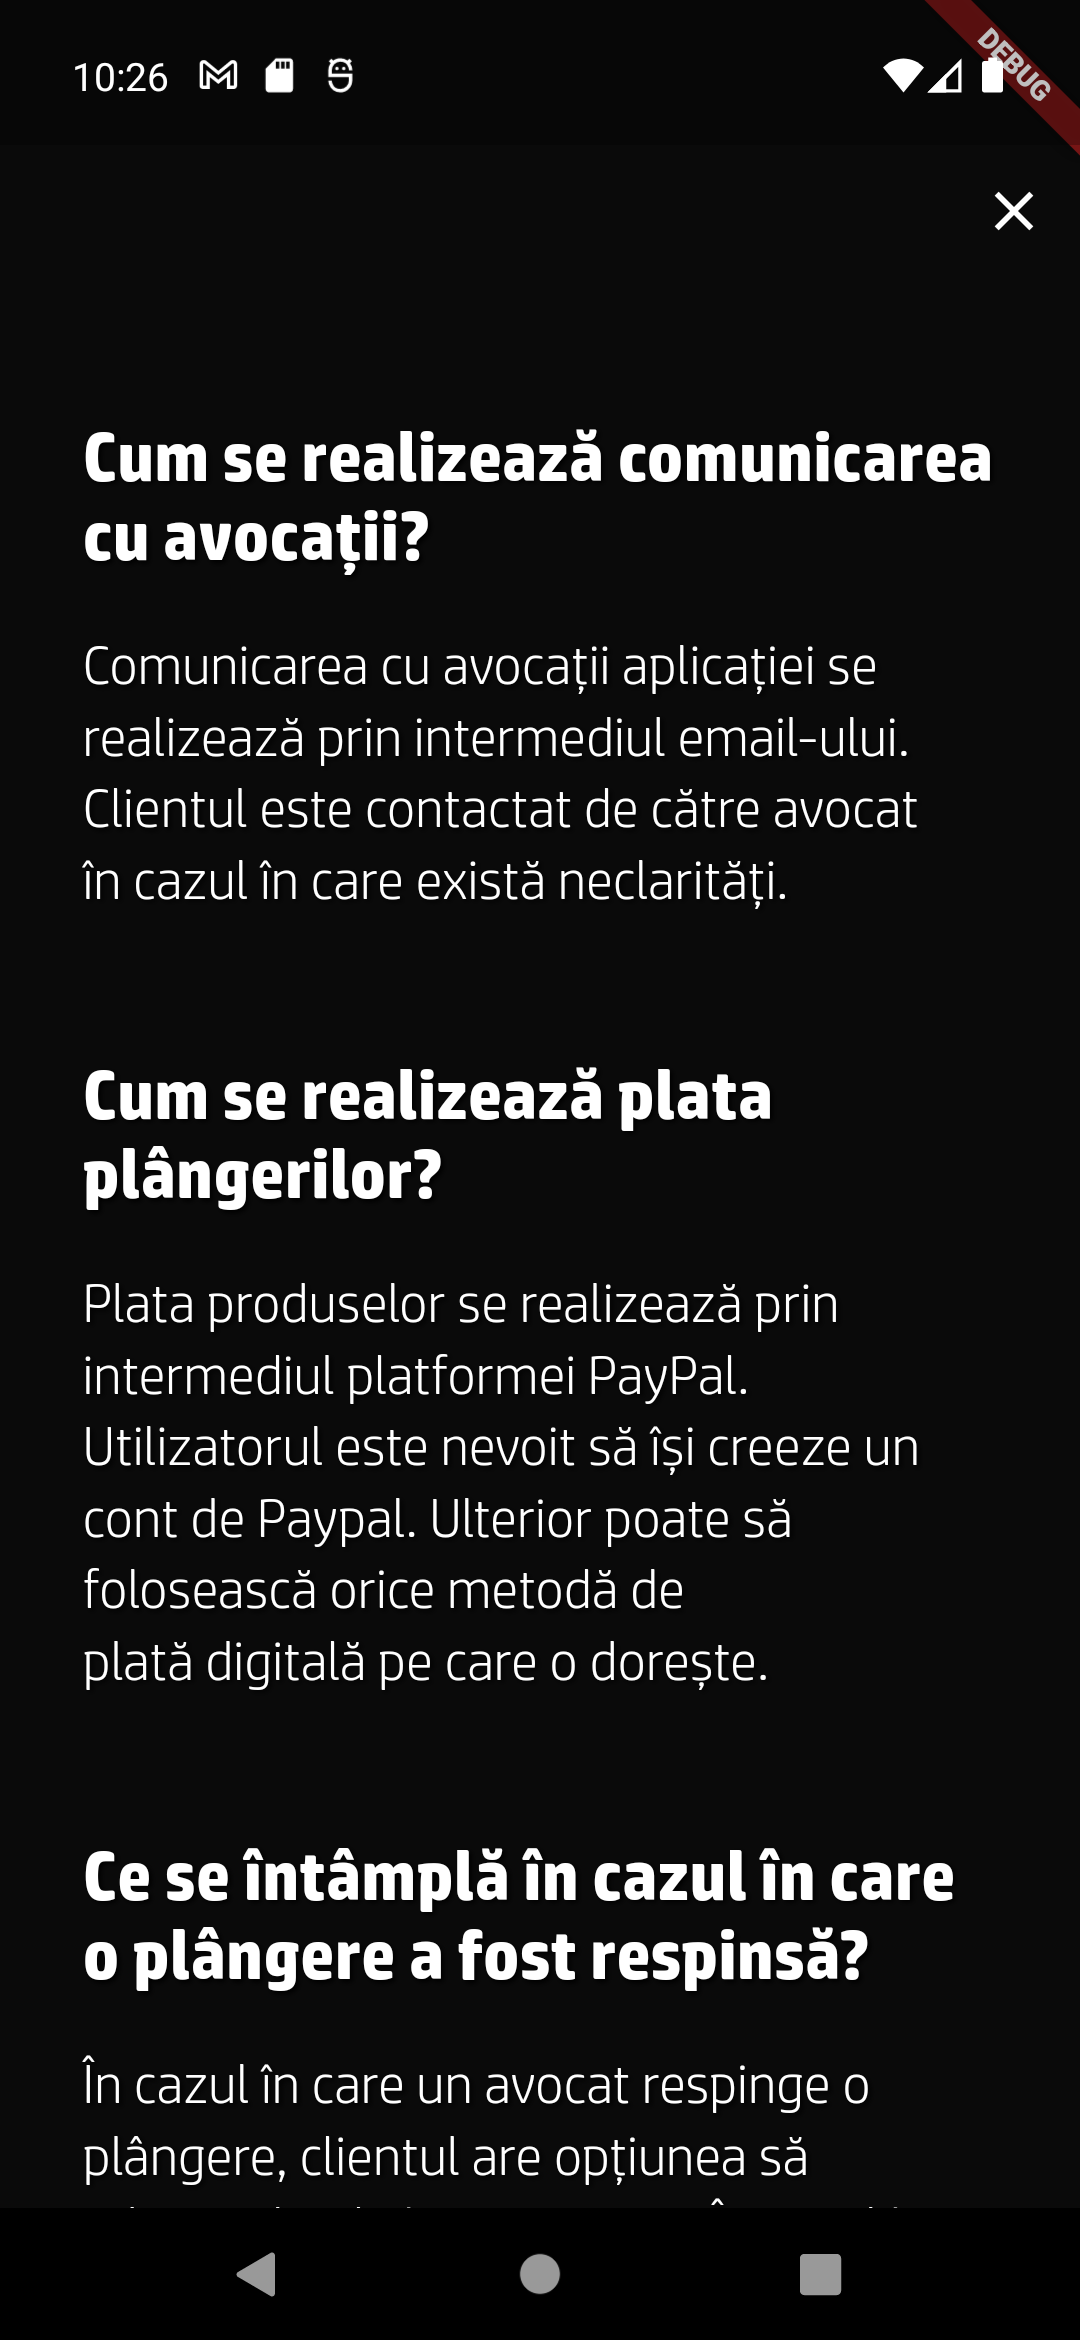
\includegraphics[width=0.23\textwidth]{images/ecran12}\label{fig:f2}}
  \hspace{0.3cm}
  \subfloat[Harta cu secțiile de poliție din proximitate]{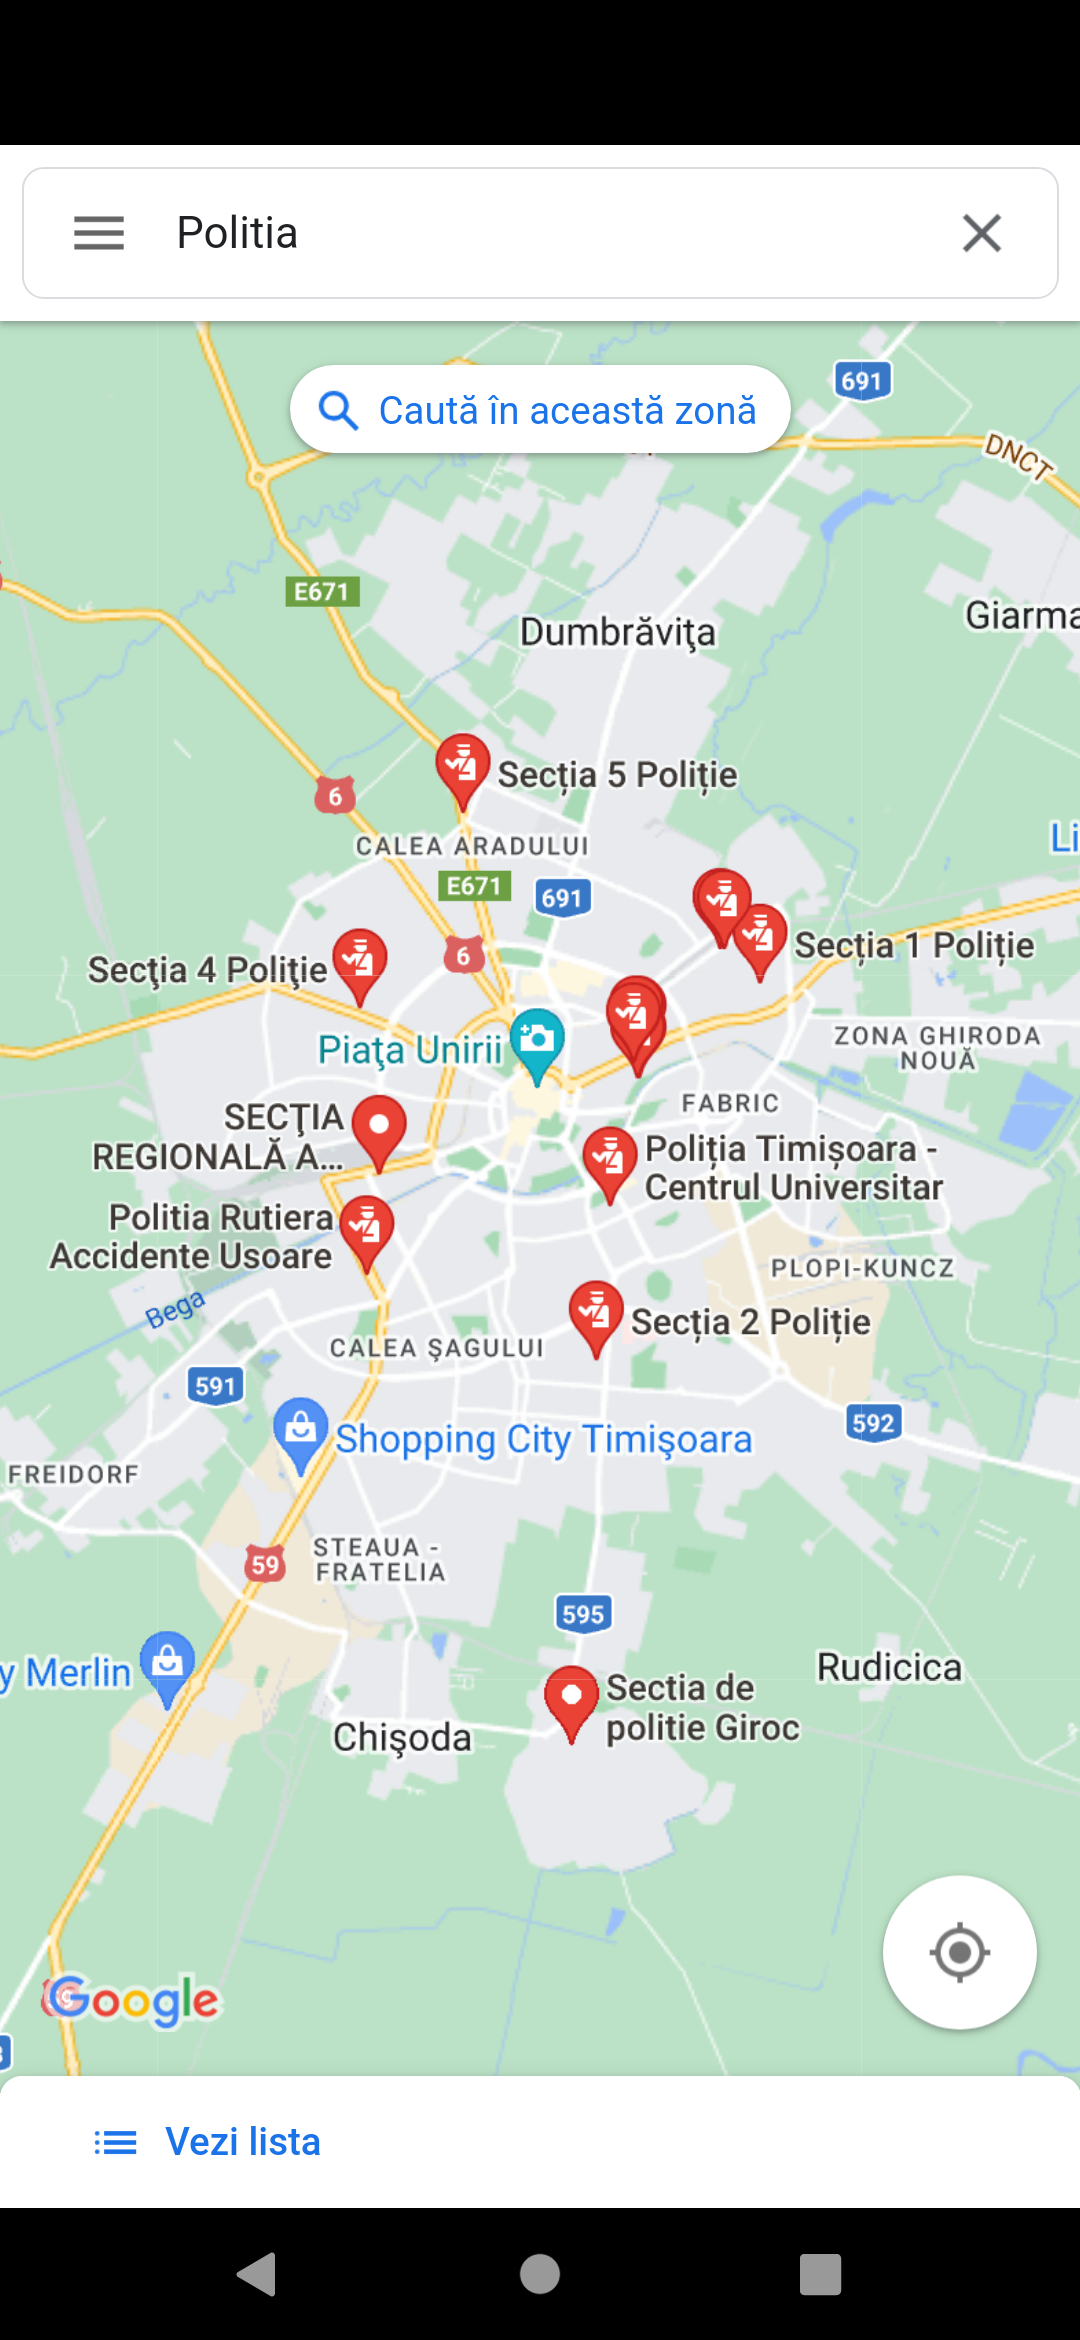
\includegraphics[width=0.23\textwidth]{images/ecran13}\label{fig:f3}}
  \caption{Diferite ecrane care prezintă funcționalitățile adiționale}
\end{figure}
\newpage
\section{Generarea plângerilor}
Ultimul aspect, dar și cel mai important, al aplicației este reprezentat de generarea plângerilor propriu-zise. Pentru ca o plângere să devină disponibilă pentru a putea să fie generată în format PDF trebuie să fie îndeplinite două cerințe: plângerea să fie plătită de către utilizator și să fie aprobată de către un avocat. Există o excepție, iar aceasta este prezentă în interfața conturilor de avocat: plângerile pot să fie generate în format PDF de către avocat în orice stadiu în care se află plângerea atâta timp cât a fost plătită și nu a fost respinsă.

Pentru ca aplicația să poată crea un fișier de tip PDF în memoria dispozitivului utilizat aplicația trebuie să ceară permisiunea de a modifica fișiere. În momentul în care un utilizator apasă pentru prima dată pe butonul de \textbf{Generare PDF} aplicația trimite o cerere de permisiune prin mecanismul clasic de permisiuni oferit de către Android. În cazul în care utilizatorul refuză să dea permisiune aplicației, aceasta trimite un Dialog Box care atenționează utilizatorul de necesitatea acestei permisiuni. În cazul în care utilizatorul dă aplicației permisiunea de scriere atunci aplicația trimite un Dialog Box care anunță utilizatorul că acțiunea a fost realizată cu succes și îl informează de locația unde a fost creat fișierul PDF. Fișierele PDF sunt create în fișierul Download al dispozitivului (/storage/emulated/0/Download).

Plângerea este generată pe baza unui model standard. În acel model există unele spații în care se introduc datele introduse în cadrul formularului de creare de plângere. Fișierul PDF este creat cu ajutorul pachetului pdf oferit de către Flutter. Crearea fișierului este asemănătoare cu crearea altor elemente vizuale din cadrul aplicației. Fișierul PDF este realizat cu ajutorul unor widget-uri (Text(), SizedBox(), etc.), în același mod în care au fost create și alte pagini ale aplicației. Diferența e că trebuie aranjate într-un mod în care să arate asemănător cu modelul după care este construită plângerea.

\begin{figure}[H]
  \centering
  \subfloat[Mesajul de succes afișat la generarea unei plângeri]{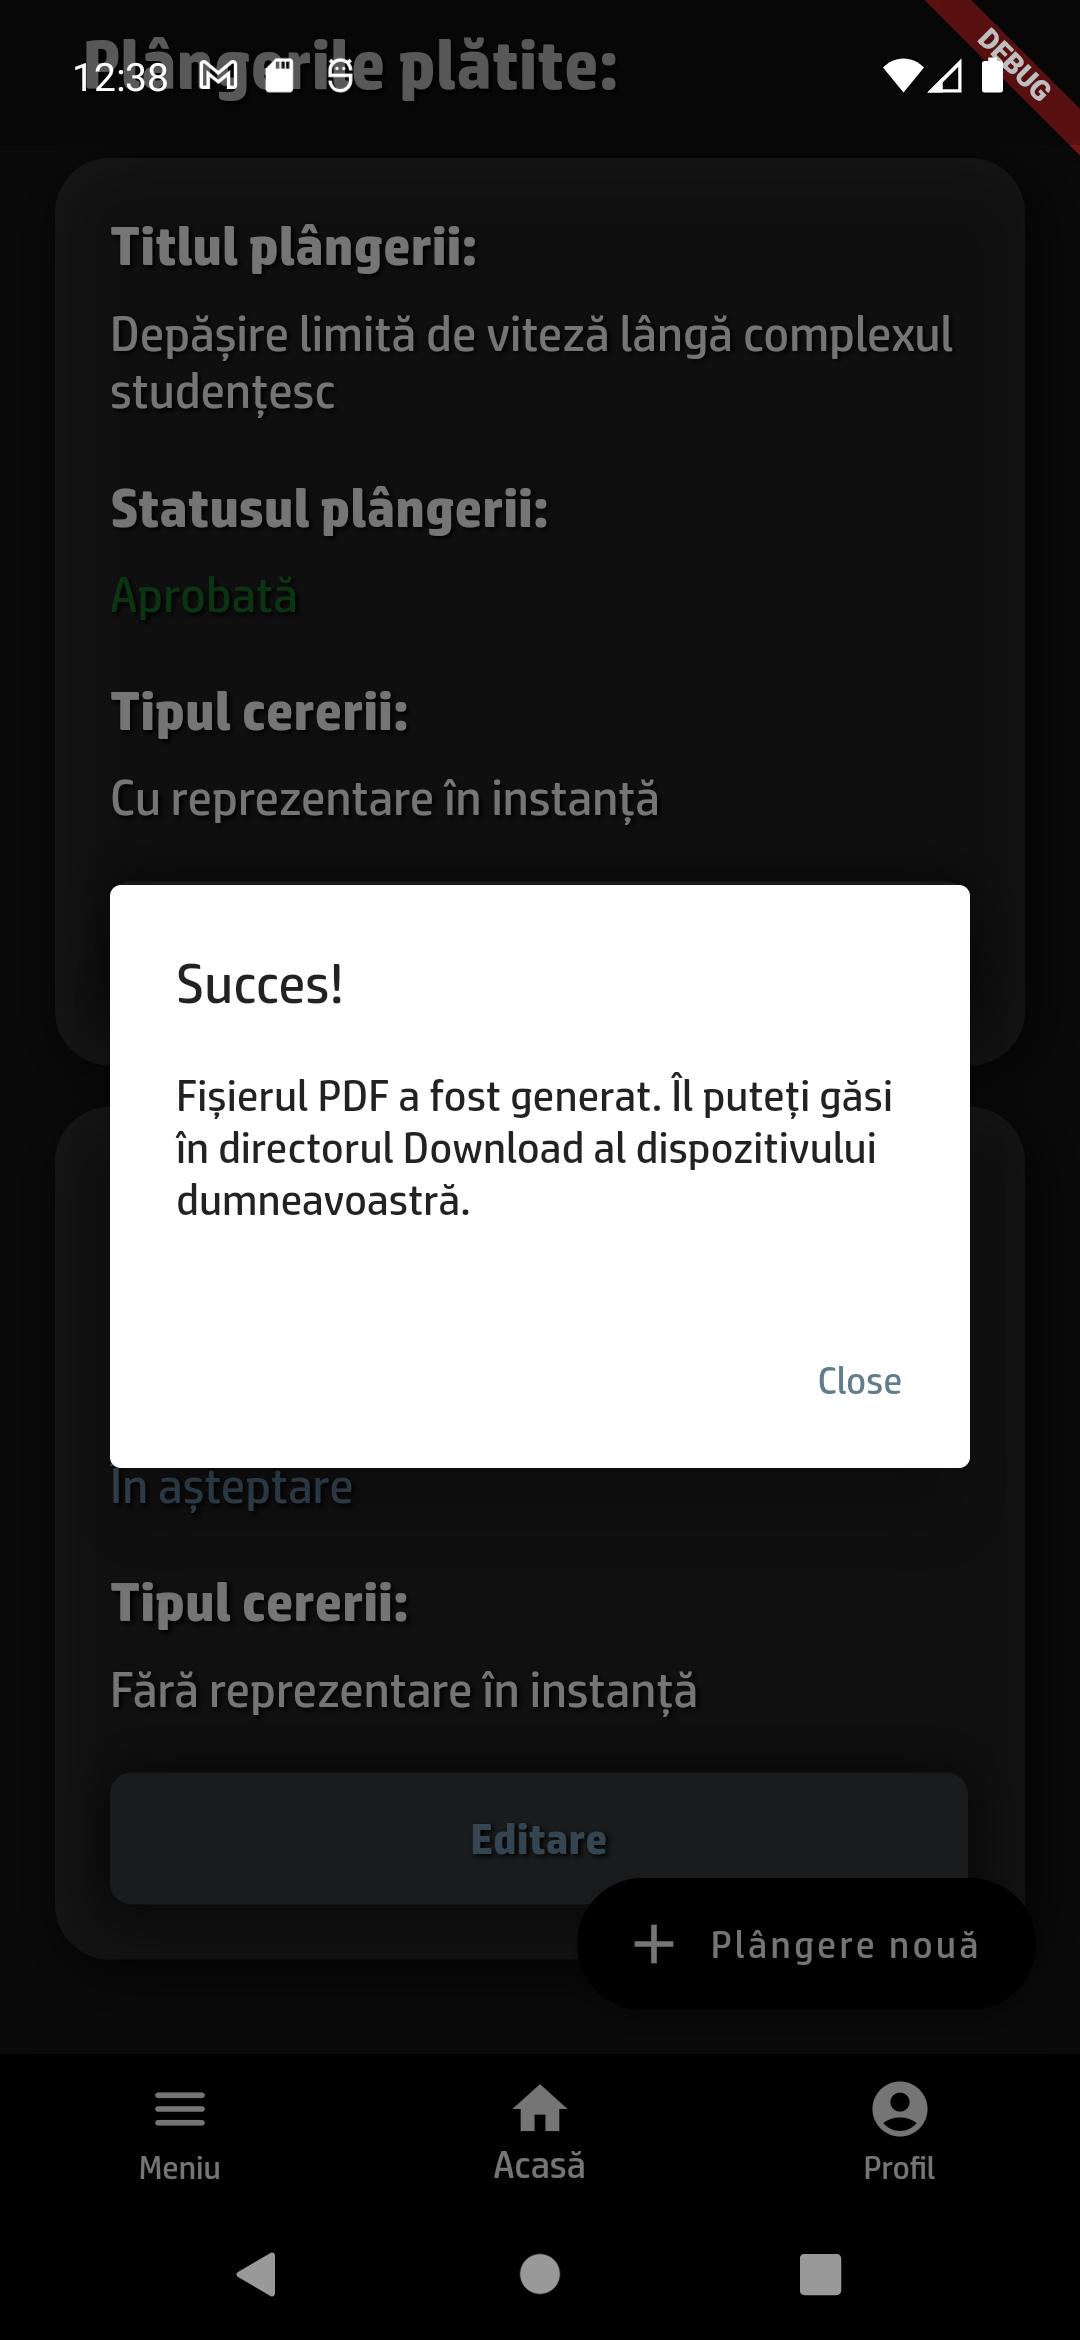
\includegraphics[width=0.23\textwidth]{images/ecran14}}
  \hspace{2.0cm}
  \subfloat[Un exemplu de plângere generată]{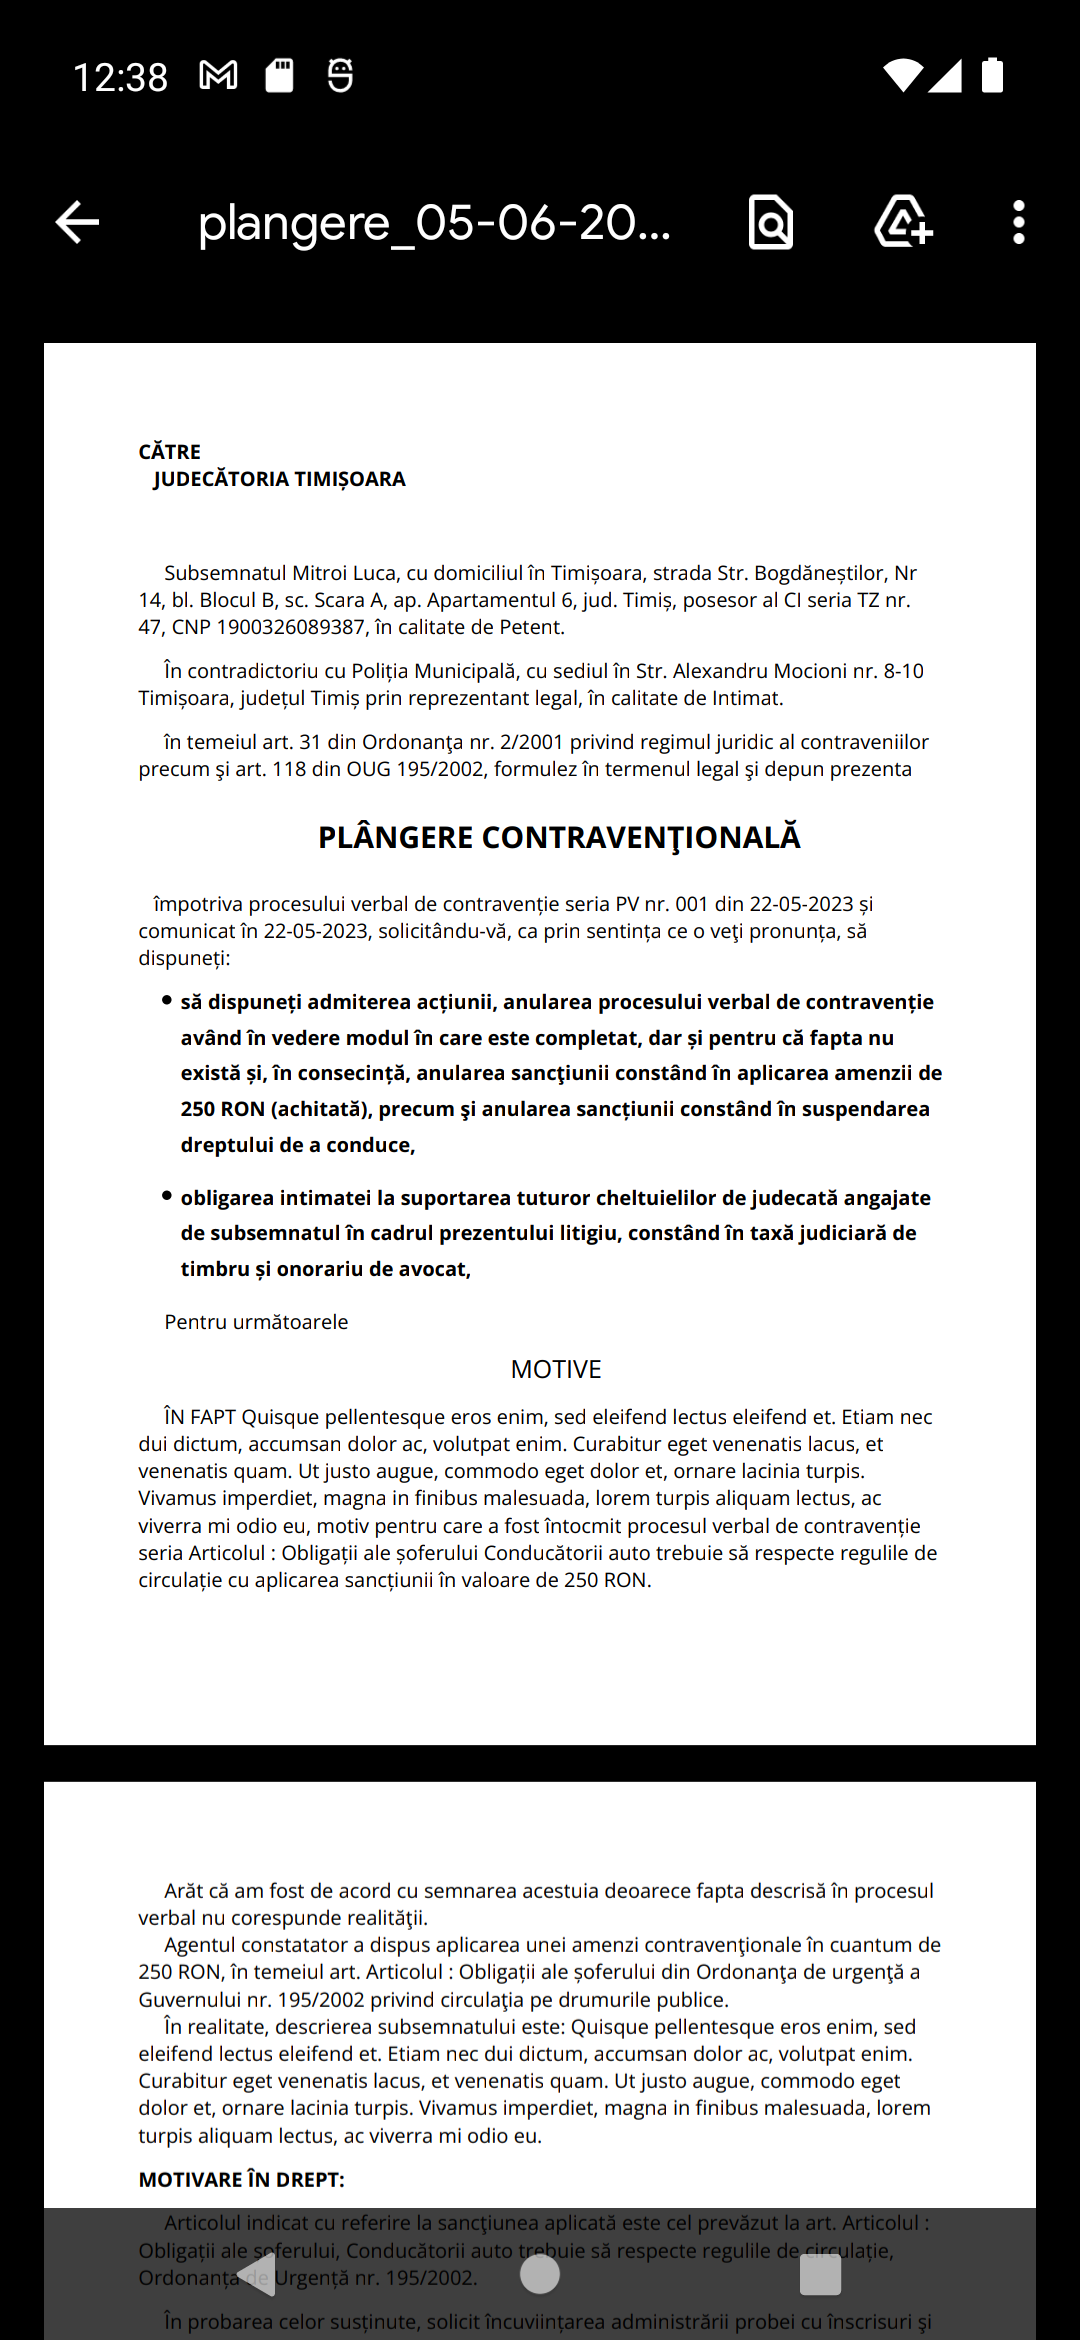
\includegraphics[width=0.23\textwidth]{images/ecran15}\label{fig:f2}}
  \caption{Generarea fișierelor PDF}
\end{figure}
\newpage
\section{Testarea aplicației}
\vspace{20pt}
Pentru asigurarea funcționării corecte a aplicației, aceasta a fost testată pentru identificarea posibilelor erori care ar putea incomoda utilizatorul, sau chiar să îi aducă probleme reale. Datorită faptului că acest proiect prelucrează informații sensibile, dar și returnează documente care urmează să fie utilizate în cadrul unui proces legal, este foarte important ca aplicația să funcționeze în parametrii normali.

Prima componentă care a fost testată a fost cea legată de conturile de utilizator. Este foarte important ca baza de date să permită existența unor utilizatori unici, pentru a asigura integritatea datelor stocate, precum și menținerea identității persoanelor cu care comunică avocații. În momentul în care utilizatorul încearcă să creeze un cont cu o adresă de mail care deja este existentă, baza de date verifică această unicitate, returnând un mesaj de eroare în cazul în care această adresă a mai fost utilizată. În acest caz nu se creează un cont nou. Același mecanism este utilizat și pentru funcționalitatea de modificare a informațiilor utilizatorilor deja existenți. Pentru o testare mai completă a funcționării procesului de creare al unor conturi de utilizator, au fost create numeroase conturi, în cadrul cărora s-au editat și datele de identificare de numeroase ori, pentru a asigura funcționarea corectă a apelurilor REST API. Majoritatea conturilor au fost șterse ulterior, acestea fiind create doar în scop de testare.

O altă parte importantă care a fost testată este legată de datele introduse de către utilizator în cadrul formularului utilizat pentru crearea unei plângeri. Un aspect care a necesitat un nivel mai mare de atenție este legat de trimiterea fiecărui câmp realizat în interfața vizuală către câmpul corespunzător din baza de date. Având în vedere că formularul are multe câmpuri, au fost necesare mai multe verificări pentru a asigura că datele din fiecare câmp sunt introduse în baza de date corect. În mod similar, au fost verificate și câmpurile din formularul asociat editării plângerilor, pentru a fi asigurată funcționalitatea operațiilor de tip patch, pentru a asigura ordinea corectă a datelor. 

Pentru testarea sistemului de plăți a fost creat un cont de dezvoltator pe platforma PayPal. Acesta permite simularea unei tranzacții fără ca dezvoltatorul să fie nevoit să facă o plată cu bani reali de fiecare dată când dorește să testeze sau să simuleze mecanismul de plată din cadrul aplicației acestuia. În același mod a fost testat și sistemul de plată din această aplicație, folosind sume de bani fictive pentru a demonstra validarea unei tranzacții urmată de schimbarea statusului unei plângeri din neachitată în achitată.

Pentru asigurarea funcționării întregii aplicații, au fost folosite de un număr mare de ori toate funcțiile acesteia, simulând comportamentul unui potențial client, respectiv unui potențial avocat. Au fost create conturi de utilizator, au fost accesate toate ecranele care conțin informații utile, au fost create diverse plângeri, care au fost verificate și în baza de date precum și în endpoint-uri, au fost editate datele din aceste plângeri și a fost simulat sistemul de plăți. În cadrul contului de avocat au fost aprobate și dezaprobate mai multe plângeri fictive, pentru a testa schimbarea statusului acestora respectiv trimiterea mail-urilor de confirmare în legătură cu statusul plângerii. A fost testată și generarea de fișiere PDF atât pe conturile de client, cât și pe cele de avocat. În testarea acestor funcționalități au fost folosite mai multe dispozitive Android, atât fizice, cât și mașini virtuale. 
\newpage
\chapter{Concluzii și direcții viitoare de dezvoltare}

\section{Concluzii}

Aplicația \textbf{e-Lawyer} vine ca o soluție a unei probleme care afectează un număr mare de oameni: modul complicat în care încă se realizează procesul de contestare al unei amenzi rutiere. Acest lucru determină un număr destul de mare de oameni să renunțe în a căuta dreptatea, ceea ce îi face să piardă sume semnificative de bani, să piardă accesul la carnetul de conducere (care pentru un număr semnificativ de persoane este vital pentru a realiza activitățile de zi cu zi), sau chiar să ajungă să aibă probleme legale reale. O altă problemă este reprezentată de faptul că oamenii de multe ori nu știu să completeze datele necesare în mod corect, ceea ce poate să îi determine să piardă cazul, iar multe persoane nici nu se gândesc să apeleze la alte persoane competente în domeniu pentru a valida informațiile.

Soluția cu care vine aplicația \textbf{e-Lawyer} este reprezentată de un serviciu care pe lângă că simplifică acest proces semnificativ, și oferă ajutor din partea unor avocați care ajută la formarea unei plângeri cât mai corecte și complete pentru o șasă cât mai mare de câștigare a cazului. Aplicația este disponibilă pe dispozitivele mobile bazate pe sistemul de operare Android. Decizia de a dezvolta aplicația pentru aceste dispozitive este legată de numărul mare de oameni care dețin telefoane mobile inteligente, aceasta fiind o piață imensă, care totuși încă este în continuă dezvoltare. Prin digitalizarea unui serviciu care inițial era înrădăcinat în metode vechi, foarte complicate și prin care se pierdea foarte mult timp, acesta devine mult mai accesibil și mai ușor de utilizat decât era în trecut. 

Aplicația oferă un formular standard, simplu de urmărit, în care sunt încărcate datele legate de amenda rutieră. Aceste date sunt ulterior salvate prin intermediul unui cont de utilizator, pentru o stocare ulterioară, ușor de utilizat. Serviciile aplicației trebuie să fie plătite de către utilizatori, deoarece aceștia sunt asistați de către niște avocați care le validează datele și decid dacă se poate continua cu cazul mai departe sau nu. Un alt serviciu oferit de către aplicație este reprezentat de faptul că, la alegerea utilizatorului, aplicația poate să desemneze un avocat care să asiste utilizatorul în sala de judecată, însă costul de utilizare crește în acest caz.

În dezvoltarea aplicației a fost utilizat framework-ul Flutter al limbajului Dart pentru componenta de Frontend, și Node.js pentru crearea părții de Backend. Conexiunea dintre aceste două componente este facilitată de REST API. Flutter este una din cele mai bune alternative pentru dezvoltarea de aplicații mobile, deoarece oferă o gamă mare de instrumente moderne care ajută la dezvoltarea unor proiecte foarte profesioniste. Framework-ul este în continuă dezvoltare, ceea ce înseamnă că are suport pentru cele mai actuale tehnologii, putând să se dezvolte aplicații care satisfac toate cerințele actuale din piață.

În final, proiectul \textbf{e-Lawyer} a ajuns într-un punct în care toate funcționalitățile sale au fost implementate, fiind într-un punct în care poate să fie lansat pe piață pentru a putea să fie utilizat de oameni.  

\section{Direcții viitoare}
În principal, direcțiile viitoare legate de această aplicație sunt legate de publicarea acesteia. În primul rând trebuie să fie finalizate toate aspectele legale pentru ca aplicația să poată să funcționeze în conformitate cu toate normele legale din România. Trebuie definitivate toate aspectele legate de colectarea datelor ale utilizatorilor. Alt aspect care trebuie să fie definitivat este legat de profitul pe care îl generează aplicația. Trebuie să se definitiveze toate taxele necesare care trebuie să fie plătite statului. Pe de altă parte, trebuie stabilit un preț final pentru fiecare serviciu oferit de aplicație precum și partea pe care o va lua fiecare avocat pentru contribuția lor, aceasta fiind una fundamentală pentru funcționarea normală a aplicație.

Un alt aspect care trebuie abordat este modul în care aplicația este distribuită. În momentul de față aplicația este instalată prin intermediul unui fișier apk care a fost generat în urma compilării întregului proiect. Această metodă nu este foarte optimă deoarece pentru a putea instala o aplicația prin intermediul unui fișier apk utilizatorul trebuie să modifice niște setări ale telefonului legate de instalarea aplicaților din afara platformei Google Play. Altă problemă în abordarea curentă este că aplicația nu se află pe nicio platformă de distribuire a aplicațiilor. De aceea, cea mai potrivită abordare este ca aplicația să fie încărcată pe Google Play. Pentru a putea încărca o aplicație pe această platformă, trebuie creat un cont de dezvoltator, și trebuie să fie plătită o taxă unică în valoare de 25 de euro. În momentul în care aplicați se află pe Google Play, aceasta este mai ușor de găsit, și respectă toate normele de securitate ale sistemului de operare Android.

O altă idee pentru viitor este portarea aplicației de pe Android pe iOS. Acest lucru nu este complicat, deoarece aplicația este dezvoltată în Flutter, ceea ce înseamnă că este același cod atât pentru Android, cât și pentru iOS. Singura diferență este legată de câteva proprietăți specifice fiecărui sistem de operare care trebuie modificate în parte pentru asigurarea funcționării corecte a aplicației. Singura problemă reală cu această idee este că Apple nu permite crearea de aplicații pentru iOS de pe Windows, ceea ce înseamnă că este nevoie ca tot proiectul să fie mutat pe un dispozitiv care rulează sistemul de operare Macintosh.


\bibliography{mybib}
\bibliographystyle{ieeetr}
\addcontentsline{toc}{chapter}{Bibliografie}

\end{document} 